%% Supplementary material for the Elsevier CAS submission.
\documentclass[a4paper,fleqn]{cas-sc}

\usepackage[numbers,sort&compress]{natbib}
\usepackage{graphicx}
\usepackage{microtype}
\usepackage{float}
\usepackage{xcolor,booktabs,longtable,array,amsmath,amssymb}
\makeatletter
\DeclareRobustCommand{\rev}[1]{{\color{red}\def\@citecolor{black}\def\@linkcolor{red}\def\@urlcolor{red}#1}}
\let\unmarkedcite\cite
\renewcommand{\cite}[1]{{\color{black}\def\@citecolor{black}\unmarkedcite{#1}}}
\makeatother
\pdfstringdefDisableCommands{\def\rev#1{#1}}
\usepackage{url}
\graphicspath{{figure/}}

% Support standard figure placement options such as [t] and [H] in CAS.
\ExplSyntaxOn
\keys_define:nn { cas / fig }
  {
    t .code:n = { \tl_set:Nn \l_fig_pos_tl { t } },
    H .code:n = { \tl_set:Nn \l_fig_pos_tl { H } }
  }
\ExplSyntaxOff

\raggedbottom
\setlength{\emergencystretch}{3em}
\setlength{\parindent}{0pt}

% Suppress the CAS running-title header and replace the default author placeholder.
\shorttitle{}
\shortauthors{G. Yang et~al.}

\makeatletter
\AtEndDocument{\clearpage\immediate\write\@auxout{\string\csxdef{lastpage}{\number\numexpr\value{page}-1\relax}}}
\makeatother

\begin{document}
\rev{\hypersetup{pdftitle={Supplementary material: Cross-context ordering and prioritization of UPR-associated transcriptional responses},pdfauthor={Guang Yang, Qi Yu, Renyu Yang, Chunxue Shao, Zongnan Lyu, Ziheng Wang}}}

\begin{center}
{\Large\bfseries Supplementary material}\\[5pt]
{\large\bfseries \rev{Cross-context ordering and prioritization of UPR-associated transcriptional responses}}\\[5pt]
{\normalsize Guang Yang, Qi Yu, Renyu Yang, Chunxue Shao, Zongnan Lyu and Ziheng Wang}
\end{center}

\vspace{2pt}
\setcounter{figure}{0}
\renewcommand{\thefigure}{S\arabic{figure}}

\begin{figure}[H]
\centering
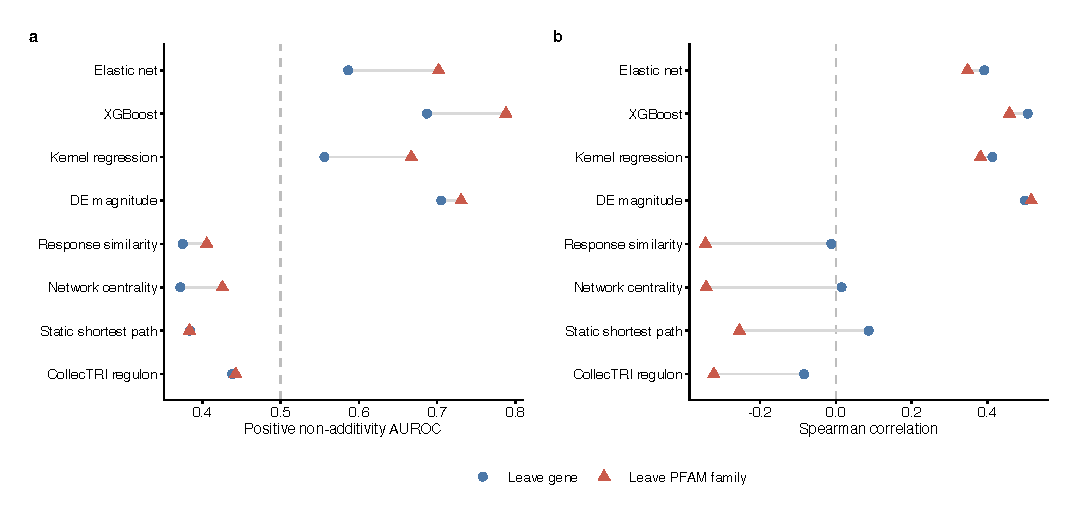
\includegraphics[width=\textwidth,height=0.52\textheight,keepaspectratio]{figure/SuppFig1_extended_baselines.pdf}
\caption{\rev{\textbf{Simple and structured baselines on identical atomic combination splits.} \textbf{a}, Positive transcriptomic non-additivity area under the receiver operating characteristic curve (AUROC) for fitted and ranking baselines under leave-gene and leave-primary-Protein families (Pfam)-family validation.} \textbf{b}, Spearman correlation between predicted and observed interaction projections. Ranking features use only matched single-perturbation responses or the public Collection of Transcriptional Regulatory Interactions (CollecTRI) prior; calibration uses training-pair outcomes only. Dashed lines denote chance AUROC or zero correlation. The CollecTRI score is not a fitted Single-Cell rEgulatory Network Inference and Clustering (SCENIC) benchmark.}
\label{fig:supp-baselines}
\end{figure}


\clearpage
\color{black}
\colorlet{scolor}{black}
\setlength{\tabcolsep}{3.5pt}
\section*{Supplementary Note S1. Source accounting, terminology and lineage sensitivity}

\rev{These notes document source-specific denominators, analysis definitions and validation results.} \rev{Supplementary data provide the retained task catalogue, gene-level evidence, negative-control statistics, intervention choices and sampling-simulation outputs.}

\paragraph{Supplementary Table S1. Source-specific denominators.}
\rev{Table S1 refers to the assay-specific task definitions and is separate from the harmonized panels and RPE1 UPR evaluation in the main text.} Cell counts refer to the six inventoried single-cell objects, not a deduplicated, jointly embedded cell atlas. The genome-wide pseudobulk breadth screen and separately processed MIX-Seq cells are outside that total. Eligible endpoint tasks, lineage units and genome-wide targets are different units.
\begin{longtable}{p{0.29\textwidth}p{0.16\textwidth}p{0.13\textwidth}p{0.31\textwidth}}
\toprule
\rev{Resource / context} & \rev{Cells in inventory} & \rev{Eligible tasks} & \rev{Use}\\
\midrule
\endhead
\rev{Replogle K562 / CRISPRi} & \rev{310,385} & \rev{285} & \rev{Program movement}\\
\rev{Replogle RPE1 / CRISPRi} & \rev{247,914} & \rev{0} & \rev{Inventoried breadth; no eligible task}\\
\rev{Norman K562 / CRISPRa} & \rev{111,668} & \rev{269} & \rev{152 singles, 117 pairs; 131 pairs in descriptive benchmark}\\
\rev{MultiPerturb / ATRT plus mouse control spike-in} & \rev{121,651} & \rev{0} & \rev{RNA--ATAC specificity diagnostics; target assays in ATRT only}\\
\rev{LARRY cytokine} & \rev{65,075} & \rev{Not task-counted} & \rev{1,268 clone--condition units / 1,065 clones}\\
\rev{LARRY in vitro} & \rev{130,887} & \rev{Not task-counted} & \rev{1,243 clone units}\\
\rev{Six-object total} & \rev{987,580} & \rev{554} & \rev{Excludes MIX-Seq}\\
\rev{MIX-Seq / chemical and genetic} & \rev{Outside inventory} & \rev{151} & \rev{120 chemical model rows; 31 GPX4 tasks outside model table}\\
\rev{All task sources} & \rev{Distinct cell denominator} & \rev{705} & \rev{285 + 269 + 0 + 151}\\
\rev{Replogle genome-wide pseudobulk} & \rev{Outside inventory} & \rev{Not task-counted} & \rev{9,867 screened gene symbols}\\
\bottomrule
\end{longtable}
\rev{MIX-Seq program tail fractions were reconstructed from 146,228 frozen QC-scored cells.} These score-table rows are not silently added to the six-object inventory. The orthogonal Norman bulk-growth measurements annotate existing pairs and add no single-cell inventory or eligible task. \rev{The retained 705-task catalogue is a provenance-level union; it does not align source-specific endpoint spaces.} \rev{The original agreement-only catalogue contained 715 tasks, including ten MultiPerturb targets that failed the additional specificity criterion.} In particular, RNA programs, lineage probabilities, Norman response basins and joint RNA--ATAC movement are not interchangeable numerical targets.

\paragraph{Source-to-analysis workflow.}
The diagram records analysis branches rather than implying a shared embedding. Public raw matrices remain at their original repositories. Frozen intermediate scores and sufficient summaries are retained for exact numerical reproduction.

\begin{center}\scriptsize
\begin{tabular}{@{}c c c c c@{}}
\fbox{\parbox{.19\textwidth}{Replogle\newline Figshare 20029387}}&\mbox{\texttt{->}}&\fbox{\parbox{.31\textwidth}{Cell QC; within-GEM program selection; count, interval and nuisance gates}}&\mbox{\texttt{->}}&\fbox{\parbox{.27\textwidth}{285 endpoint tasks; gene evidence\newline RPE1: inventory only}}\\[8pt]
\fbox{\parbox{.19\textwidth}{Norman\newline GSE133344}}&\mbox{\texttt{->}}&\fbox{\parbox{.31\textwidth}{Simplify constructs; log1p CP10k; 8 technical GEMs; count and agreement gates}}&\mbox{\texttt{->}}&\fbox{\parbox{.27\textwidth}{269 tasks; 131-pair descriptions and predictions; endpoint graph}}\\[8pt]
\fbox{\parbox{.19\textwidth}{MIX-Seq\newline Figshare 10298696}}&\mbox{\texttt{->}}&\fbox{\parbox{.31\textwidth}{Matched controls; program tails; task branch: 100 cells/arm and SE; duration branch: all matched pairs}}&\mbox{\texttt{->}}&\fbox{\parbox{.27\textwidth}{151 tasks; 120 chemical model rows; 158 duration contrasts}}\\[8pt]
\fbox{\parbox{.19\textwidth}{LARRY\newline GSE140802}}&\mbox{\texttt{->}}&\fbox{\parbox{.31\textwidth}{Day-2 clone baselines; day-6 branch counts; condition-specific neighbours}}&\mbox{\texttt{->}}&\fbox{\parbox{.27\textwidth}{Local covariance rank; clone inference; resource transfer}}\\[8pt]
\fbox{\parbox{.19\textwidth}{MultiPerturb\newline GSE277747}} & \mbox{\texttt{->}} & \fbox{\parbox{.31\textwidth}{Context controls; cell/guide support; guide agreement; non-targeting construct test}} & \mbox{\texttt{->}} & \fbox{\parbox{.27\textwidth}{0 retained tasks; specificity diagnostics; no supported modality roles}}\\
\end{tabular}
\end{center}

\paragraph{Supplementary Table S2. Sequential condition-level gates.}
Counts show the remaining conditions after each listed gate, in the displayed order. They are not independent exclusion categories. Preprocessed cell QC precedes these task gates. All exclusion reasons and condition identities remain available in the machine-readable catalogue.
\begin{longtable}{p{0.21\textwidth}p{0.62\textwidth}p{0.1\textwidth}}
\toprule
\rev{Source} & \rev{Sequential gate} & \rev{Remaining}\\
\midrule
\endhead
\rev{Replogle K562} & \rev{Candidate conditions} & \rev{2057}\\
\rev{Replogle K562} & \rev{Target cells $\geq100$} & \rev{1156}\\
\rev{Replogle K562} & \rev{At least three GEM groups} & \rev{1156}\\
\rev{Replogle K562} & \rev{Target-selection agreement $\geq0.60$} & \rev{1118}\\
\rev{Replogle K562} & \rev{Positive held-out effects in at least 60\% of groups} & \rev{675}\\
\rev{Replogle K562} & \rev{Positive lower 95\% $t$ limit} & \rev{577}\\
\rev{Replogle K562} & \rev{BH $q<0.05$} & \rev{522}\\
\rev{Replogle K562} & \rev{Nuisance separation} & \rev{285}\\
\rev{Norman} & \rev{Candidate conditions} & \rev{283}\\
\rev{Norman} & \rev{At least 30 cells} & \rev{283}\\
\rev{Norman} & \rev{At least six GEM cosines $>0.20$} & \rev{283}\\
\rev{Norman} & \rev{Nuisance separation} & \rev{283}\\
\rev{Norman} & \rev{At least 100 cells for task catalogue} & \rev{269}\\
\rev{MIX-Seq} & \rev{Candidate conditions} & \rev{1115}\\
\rev{MIX-Seq} & \rev{At least 100 cells in both arms} & \rev{151}\\
\rev{MIX-Seq} & \rev{Maximum program SE $\leq0.10$} & \rev{151}\\
\rev{MultiPerturb} & \rev{Candidate conditions} & \rev{99}\\
\rev{MultiPerturb} & \rev{Target cells $\geq100$} & \rev{80}\\
\rev{MultiPerturb} & \rev{At least two guides} & \rev{55}\\
\rev{MultiPerturb} & \rev{At least 15 cells in every guide} & \rev{28}\\
\rev{MultiPerturb} & \rev{All guide nuisance gates} & \rev{27}\\
\rev{MultiPerturb} & \rev{RNA median cosine $>0.10$} & \rev{18}\\
\rev{MultiPerturb} & \rev{ATAC median cosine $>0.10$} & \rev{10}\\
\rev{MultiPerturb} & \rev{Non-targeting-construct BH $q<0.05$} & \rev{0}\\
\bottomrule
\end{longtable}
\paragraph{Operational terminology.}
\begin{longtable}{p{.24\textwidth}p{.68\textwidth}}
\toprule
\rev{Term} & \rev{Operational meaning}\\ 
\midrule
\endhead
\rev{\textbf{Measured endpoint contrast:}} & \rev{difference between sampled populations under a recorded intervention and a matched control; it does not track the same individual cells.}\\
\rev{\textbf{State-transition task:}} & \rev{historical catalogue label for a complete source--intervention--endpoint condition. It need not represent a stable fate transition.}\\
\rev{\textbf{Local effective rank:}} & \rev{entropy rank of covariance among neighbouring clones' descendant branch-probability vectors. It measures variation of probability vectors, not the number of fates available to an individual clone.}\\
\rev{\textbf{Response basin / target state:}} & \rev{a descriptive Norman cluster / a source-specific endpoint definition. Neither is independently validated as an attractor or committed fate.}\\
\rev{\textbf{Endpoint-graph component:}} & \rev{a connected component of an endpoint-similarity graph. No time-ordered biological route is measured.}\\
\rev{\textbf{Relative effort:}} & \rev{intervention size divided by squared response magnitude. It is an empirical ranking proxy, not physical control energy.}\\
\rev{\textbf{Empirical reachability:}} & \rev{would require intervention-conditional attainment of a specified target within a horizon; persistence after withdrawal requires additional evidence. This study does not estimate that probability.}\\
\rev{\textbf{Dynamical controllability:}} & \rev{a property of an identified dynamical system and its admissible inputs. It is not established by endpoint similarity or local covariance rank.}\\
\bottomrule
\end{longtable}

\paragraph{LARRY construction and independence.}
The cytokine and in vitro data are related experimental arms of the same Weinreb et al. study (GSE140802). They do not provide independent study replication. Day-2 cells define clone baselines; day-6 descendants define condition-specific branch counts. Supplied labels map to basophil, dendritic, eosinophil, erythroid, lymphoid, mast, megakaryocyte, monocyte, neutrophil, plasmacytoid dendritic, undifferentiated or other categories, retaining observed terminal categories (ten cytokine, eleven in vitro). A clone's branch probability is its branch count divided by all descendants in that future condition. The frozen input retains exact integer branch counts and the 41 selected baseline axes. Day-2 baseline counts differ from the upstream table's all-preterminal-cell counts.

Frozen pathway/regulon scores used univariate linear-model scoring (\texttt{decoupler.mt.ulm}, minimum five targets, normalized expression), with mouse PROGENy top-500, CollecTRI and Hallmark snapshots. Stress is the mean of the HYPOXIA, REACTIVE\_OXYGEN\_SPECIES\_PATHWAY and UNFOLDED\_PROTEIN\_RESPONSE axes. Those three axes are excluded from every stress neighbourhood. Network revisions are not substituted for the frozen numeric axes.

The extended model adds $\log(1+n_{day2})$, $\log(1+n_{day6})$, $\log(1+\text{mean detected genes})$ and dominant baseline-library indicators to the original five state covariates and future condition. The expression matrices are normalized; detected genes and mitochondrial expression fraction are quality proxies, and raw sequencing depth is unavailable. Mitochondrial coefficients $-5.73$ and $-14.76$ are per unit fraction on a 0--1 scale; per percentage point they are $-0.0573$ and $-0.1476$. Figure 2c uses predictor-standard-deviation scaling. Its bars are asymptotic coefficient $\pm1.96$ SE intervals, whereas primary original $P$ values use 999 clone-level partial-residual permutations.

Twelve specifications comprise the original geometry; $k=15,30,60$; 5, 10 or the original 15 principal components; pathway-only, regulon-only or joint axes; standardized axes without PCA; and diagonal covariance shrinkage $(1-\lambda)C+\lambda\operatorname{diag}(C)$ for $\lambda=0.01,0.05,0.20$. Branch-support cutoffs 0.01, 0.05 and 0.10 affect thresholded branch counts but do not enter rank. All extended-adjustment rank coefficients are negative across these settings. The original stress geometry is reproduced to maximum absolute discrepancy $1.6\times10^{-14}$.

Full-pipeline percentile intervals resample complete clones, retaining their future-condition records, and recompute scaling, PCA, neighbours and covariance in 200 draws. Extended slopes are $-0.0926$ and $-0.3400$, with intervals $[-0.203,-0.0457]$ and $[-0.418,-0.179]$. These quantify within-study sampling sensitivity, not between-experiment uncertainty. A natural spline with three degrees of freedom describes nonlinearity; it does not test a causal threshold. Adjusted 95th-versus-5th percentile stress contrasts are $-0.302$ and $-0.928$.

Descendant rarefaction samples exact branch counts without replacement at $m=2,5,10$, with 100 draws per setting. The retained units are 752, 296 and 92 of 1,268 cytokine units, and 921, 536 and 284 of 1,243 in vitro units. Each retained subset has a separately recomputed neighbourhood and an unsampled reference. All $m=2$ and $m=5$ stress coefficients are negative. At $m=10$, 89/100 cytokine estimates are positive (median $+0.0412$), and the same retained unsampled subset already has slope $+0.0358$. The in vitro median remains negative ($-0.0851$). This is strong subset dependence, not proof that sampling alone causes reversal. Individual-clone entropy and observed branch counts have in vitro intervals spanning zero after adjustment, reinforcing their distinction from neighbour covariance rank.

\paragraph{Measured-quality balance and common support.}
High stress is above the resource-specific median across unique clones. Initial weights are the reciprocal of each clone's number of future-condition records. A weighted logistic model estimates high-stress probability $e_i$; overlap weights multiply the initial weight by $1-e_i$ for high stress and $e_i$ for low stress. The quality model includes categorical baseline count, natural splines of log(1+descendant count) (2 degrees of freedom), log(1+mean detected genes) and mitochondrial fraction (3 each), baseline library and future condition. The stronger specification adds cycle, chromatin-regulator and metabolic scores; this may also condition on biology. Maximum absolute standardized mean differences over model terms were below $1.7\times10^{-7}$ after weighting. This balances modeled covariate means, not every aspect of measurement quality, and does not identify a causal stress effect.

\begin{longtable}{p{.19\textwidth}p{.22\textwidth}p{.29\textwidth}p{.19\textwidth}}
\toprule
\rev{Resource} & \rev{Balance model} & \rev{High-minus-low rank [95\% interval]} & \rev{ESS high / low}\\
\midrule
\endhead
\rev{Cytokine} & \rev{Quality/abundance} & \rev{$-0.168$ [$-0.250,-0.087$]} & \rev{402 / 407}\\
\rev{Cytokine} & \rev{Quality + states} & \rev{$-0.135$ [$-0.212,-0.052$]} & \rev{365 / 379}\\
\rev{In vitro} & \rev{Quality/abundance} & \rev{$-0.073$ [$-0.186,0.030$]} & \rev{305 / 337}\\
\rev{In vitro} & \rev{Quality + states} & \rev{$-0.089$ [$-0.209,0.023$]} & \rev{278 / 311}\\
\bottomrule
\end{longtable}
Intervals use 499 complete-clone bootstrap draws, all converged, with weights re-estimated but the original geometry, spline basis and median threshold fixed. They do not replace the 200-draw full-pipeline intervals for continuous slopes. Fixed-weight cluster-sandwich intervals are supplied separately; they are wider and cross zero for the stronger cytokine specification. Re-estimating weights restores modeled balance within bootstrap draws, so the procedures need not agree. Neither establishes guaranteed coverage or independent replication. In the stronger in vitro model, 364/1,243 units had $e_i<0.05$ or $e_i>0.95$; inference concerns the overlap population.

Keeping original ranks and selecting only cytokine queries with at least ten descendants gives a positive slope $+0.1137$, versus $+0.0358$ when the selected subset also rebuilds geometry. The retained subset changes from 35.3\% to 57.6\% M-csf and from 46.2\% to 18.5\% full cocktail. A separate diagnostic fixes the original PCA and all queries while restricting descendant-probability donors to at least ten descendants; its slope is $+0.0171$, using 10--21 neighbours after the availability cap. Thus the reversal is not solely caused by refitting PCA; selection and neighbourhood support both matter.

\paragraph{Paired cytokine-condition observations.}
Full cocktail shares 109, 46 and ten clones with M-csf, G-csf and Epo, respectively. Each pair has identical recorded baseline stress and quality scores. Mean within-clone Jensen--Shannon divergences between day-6 branch distributions are 0.199, 0.203 and 0.479 nats. Finite descendant sampling itself contributes divergence. Requiring at least two descendants in both conditions retains only 43, 16 and four pairs. An upper-tail paired label-swap diagnostic compares the squared norm of mean branch-probability displacement using 9,999 swaps, with BH correction across the three comparisons. Corrected values are 0.0165, 0.1473 and 0.1473 unrestricted, and 0.0783, 0.0906 and 0.1270 with the depth restriction. These observed context contrasts do not establish global-topology reorganization or a stress-independent mechanism. Clone identities, branch shifts, support and conditional paired-bootstrap intervals are supplied.

\clearpage
\begin{figure}[H]
\centering
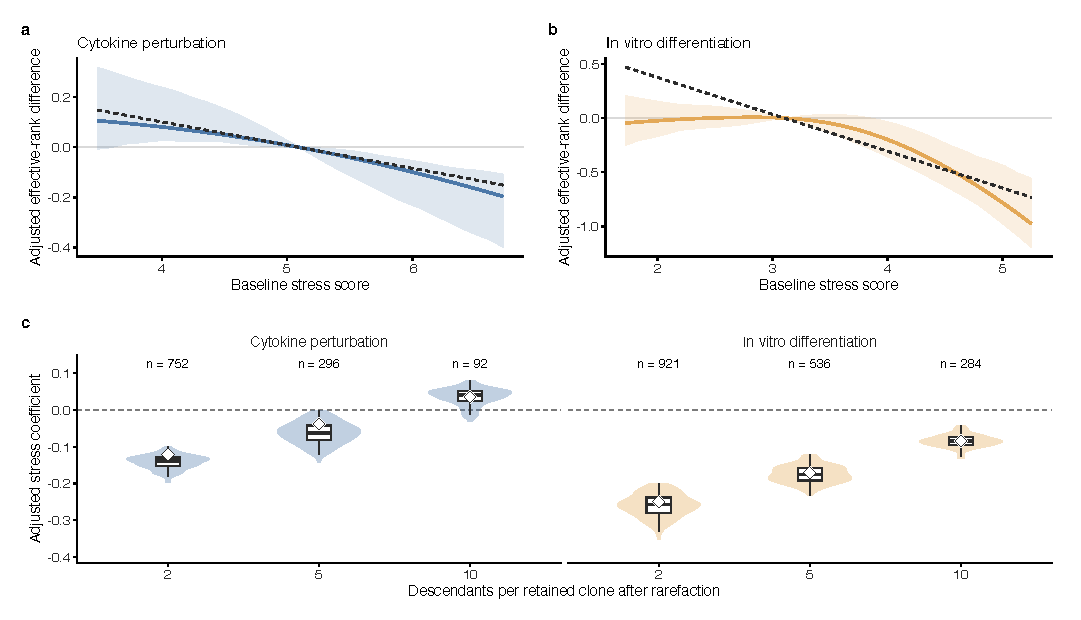
\includegraphics[width=\textwidth]{figure/SuppFigS2_lineage_sensitivity.pdf}
\caption{\textbf{Adjusted lineage associations and descendant-depth sensitivity.} \textbf{a,b}, Adjusted effective-rank contrasts relative to median stress in the cytokine and in vitro resources. Solid lines show three-degree-of-freedom natural splines; dashed lines show extended linear fits. Shading is the 95\% percentile interval from 200 complete-clone bootstrap draws, recomputing PCA, neighbours and covariance; it is not a simultaneous confidence band. \textbf{c}, Stress coefficients from 100 without-replacement descendant rarefactions at each retained depth. Violin and box distributions describe repeated computational resamples, not biological replicates; boxes show median and interquartile range. Diamonds are the unsampled retained-subset coefficients. Printed $n$ values are clone--condition units. Covariates include the original five states, baseline/descendant counts, detected-gene complexity, baseline library and future condition. The strict cytokine subset changes the coefficient's sign.}
\label{fig:supp-lineage}
\end{figure}

\section*{Supplementary Note S2. Matched prediction and selective coverage}

MIX-Seq program scores are the mean $\log(1+10^4x/L)$ over available positive genes minus the corresponding negative-gene mean (zero for an empty negative set). Exact gene membership is supplied with the code. Within matched dataset, experiment, time, task and cell line, controls are prioritized DMSO, untreated, vehicle, control; genetic controls prioritize sgLACZ over sgOR2J2. The frozen upstream catalogue requires at least 20 cells per arm. A program's threshold is its matched-control median plus $1.4826$ times the median absolute deviation. \rev{With $s$ treated scores exceeding this threshold among $n$ observed scores,
{}
{\color{red}
\[
p=\frac{s+1}{n+2},\qquad \mathrm{SE}=\sqrt{\frac{p(1-p)}{n+3}}.
\]
}
\rev{}
These nonexclusive transcriptional tail fractions are not death, proliferation-event or stable-fate probabilities. All 1,115 frozen tasks, counts, tail fractions and SEs were reconstructed from the scored cells (maximum fraction discrepancy $1.11\times10^{-16}$). The 0.1 prior used in the conditional-rate model and distance proxy is a separate convention, not the matched-control exceedance rate.}

The chemical model table has 1,044 conditions; 120 have at least 100 cells per arm, and all 120 satisfy the SE gate (maximum 0.04876). Thus the SE rule removes no additional chemical benchmark cases. Thirty-one eligible genetic GPX4 tasks lack the DMSO-baseline model representation. The 120 chemical tasks span 41 cell lines.

The original frozen scVI representation was fitted to 21,936 QC-passing DMSO cells from 169 cell lines in 335 baseline contexts and five technical batches. The 41 benchmark lines contribute 10,006 cells in 101 contexts; the 120 primary tasks use 7,328 cells in 57 of those contexts. The recovered model checkpoint records scvi-tools 1.4.3, 30 latent dimensions, two 128-unit layers, dropout 0.1, gene-wise dispersion, negative-binomial likelihood, a normal latent distribution and observed library sizes. The source script selected 4,000 batch-aware variable genes with the Cell Ranger method after per-cell CP10k normalization and log1p transformation, then trained scVI on their unnormalized UMI counts (seed 20260713; at most 200 epochs; early-stopping patience 20; validation every five epochs; batch size 256). The archived fit ran all 200 epochs. Its context-mean latent values exactly reproduce all 1,044 chemical modeling rows. All baseline cells enter this descriptive fit before prediction splitting. Five source clusters and outcome-defined dominant-target groups are also fixed before splitting. Predictor scaling, model fitting, elastic-net tuning and training-distance thresholds are computed within training folds. This is a conditional benchmark with globally learned baseline representation and retrospective target groups, not a nested raw-count-to-prediction evaluation. The additional nested cell-line evaluation below refits baseline feature selection and scVI from the recorded QC-qualified UMI counts. Retained/excluded effect-size summaries and all observation-to-fold assignments are supplied.

For matched comparisons, both methods must accept the identical task. Confidence intervals resample 2,000 cell-line clusters, keeping all conditions from a sampled line together; fixed out-of-fold predictions are not refitted. They omit uncertainty from latent learning, model retraining and new biological experiments. Pairwise intersections and the all-model intersection are both reported. The latter contains only 17, 3 and 37 tasks for cell-line, source-state and target-state validation. Small accepted subsets, including only two accepted cell lines for the source-state conditional-rate model, give unstable uncertainty estimates.

The retained Supplementary Figure S3 curves use the original globally fitted baseline coordinates. Selective risk curves vary the uncertainty cutoff while retaining intervention-presence, training-distance and kernel-support applicability rules. They use the same selected tasks for the response model and static comparators at each cutoff. The original threshold 0.15 is heuristic; it is neither optimized here nor a calibrated confidence level. The unseen-intervention rule gives zero coverage for every response model, regardless of the uncertainty threshold. Uncertainty--error Spearman correlations among hard-supported cases vary from $-0.036$ to 0.629; this does not establish calibrated uncertainty. Overall and three endpoint-specific curves are shown in Supplementary Figure S3; zero-coverage cells remain explicit.

\paragraph{Training-only threshold selection.}
Five outer cell-line folds retain the original 120 test conditions. Four grouped inner cell-line folds within each training set generate new local-ridge, kernel and three-initialization conditional-rate predictions, with training-only scaling and distance gates. For each exploratory RMSE tolerance (0.10, 0.15 or 0.20), choose the uncertainty cutoff accepting the most inner cases while meeting the observed inner tolerance, at least ten accepted cases and three accepted lines. A fold with no qualifying cutoff abstains. Tolerances are sensitivity settings, not prespecified clinical targets or finite-sample guarantees; outer outcomes are not used to choose the cutoff.

At tolerance 0.10, local ridge accepts 19/120 outer cases (RMSE 0.1566; matched elastic net 0.1262), kernel 28/120 (0.09694 versus 0.09994), and conditional rate none. Kernel-minus-elastic RMSE difference is $-0.00300$ [95\% interval $-0.00840,0.00221$]. At tolerance 0.15, local and kernel accept 59 and 41 cases, while conditional rate accepts only five from one line, precluding a reliable across-line interval. At 0.20, conditional rate accepts 26 cases (RMSE 0.1499 versus matched elastic net 0.1120). Intervals use 2,000 line-cluster resamples conditional on the selected decisions and outer predictions; threshold selection and fitting are not repeated in this bootstrap. All 1,080 case/model/tolerance decisions and inner/outer memberships are supplied. Empirical inner risk need not transfer under a cell-line shift.

\paragraph{Alternative outer-training RNA representation.}
Selecting the 57 matched-control contexts for the 120 primary tasks from five QC DMSO matrices yields 7,328 cells across 41 lines, with all context counts matching the original endpoints. Mean per-cell log1p CP10k profiles retain 32,738 genes. Within each outer training fold, unique training contexts select the 2,000 highest-variance genes and fit centered, unscaled PCA (30 components); held-out contexts are projected only. Predictor scaling and model fitting also exclude outer-test lines. Elastic net uses $\alpha=0.5$ and grouped training-line cross-validation; PCA precedes this inner lambda tuning within the outer training set. Kernel retains the same-intervention support, distance gate and heuristic 0.15 uncertainty cutoff. Complete selected-gene lists, 45--46 training / 11--12 test contexts per fold, cell/context mapping and prediction assignments are supplied.

RNA/PCA elastic net gives RMSE 0.10531 [95\% line-cluster interval 0.09126, 0.12069] at 120/120 coverage; kernel gives 0.09397 [0.08021, 0.10853] on 98/120. Matched elastic-net RMSE on those 98 cases is 0.09687; kernel-minus-elastic difference is $-0.00290$ [$-0.00649,0.00135$]. Coverage differs substantially from the frozen-scVI benchmark. This earlier alternative uses primary-task context means rather than the full auxiliary baseline reference panel. It does not isolate a causal effect of representation architecture. The count-level scVI check below retains the fixed original QC mask and endpoint definitions.

\paragraph{Supplementary Table S3a. Overall endpoint RMSE at the original cutoff.}
Intervals are conditional 95\% percentile cell-line-cluster bootstrap intervals. Counts and coverage refer to 120 complete test conditions per axis. ``--'' denotes no accepted predictions.
\small
\begin{longtable}{p{0.15\textwidth}p{0.19\textwidth}p{0.07\textwidth}p{0.13\textwidth}p{0.36\textwidth}}
\toprule
\rev{Holdout} & \rev{Model} & \rev{$n$} & \rev{Coverage} & \rev{RMSE [95\% interval]}\\
\midrule
\endhead
\rev{Cell line} & \rev{Mean} & \rev{120} & \rev{100.0\%} & \rev{0.155 [0.119, 0.189]}\\
\rev{Cell line} & \rev{Ridge} & \rev{120} & \rev{100.0\%} & \rev{0.149 [0.132, 0.169]}\\
\rev{Cell line} & \rev{Elastic net} & \rev{120} & \rev{100.0\%} & \rev{0.100 [0.089, 0.112]}\\
\rev{Cell line} & \rev{Local ridge} & \rev{59} & \rev{49.2\%} & \rev{0.125 [0.099, 0.148]}\\
\rev{Cell line} & \rev{Kernel} & \rev{41} & \rev{34.2\%} & \rev{0.098 [0.084, 0.113]}\\
\rev{Cell line} & \rev{Rate network} & \rev{27} & \rev{22.5\%} & \rev{0.151 [0.111, 0.198]}\\
\rev{Intervention} & \rev{Mean} & \rev{120} & \rev{100.0\%} & \rev{0.162 [0.124, 0.202]}\\
\rev{Intervention} & \rev{Ridge} & \rev{120} & \rev{100.0\%} & \rev{0.171 [0.136, 0.206]}\\
\rev{Intervention} & \rev{Elastic net} & \rev{120} & \rev{100.0\%} & \rev{0.158 [0.117, 0.196]}\\
\rev{Intervention} & \rev{Local ridge} & \rev{0} & \rev{0.0\%} & \rev{--}\\
\rev{Intervention} & \rev{Kernel} & \rev{0} & \rev{0.0\%} & \rev{--}\\
\rev{Intervention} & \rev{Rate network} & \rev{0} & \rev{0.0\%} & \rev{--}\\
\rev{Source} & \rev{Mean} & \rev{120} & \rev{100.0\%} & \rev{0.156 [0.116, 0.189]}\\
\rev{Source} & \rev{Ridge} & \rev{120} & \rev{100.0\%} & \rev{0.155 [0.137, 0.174]}\\
\rev{Source} & \rev{Elastic net} & \rev{120} & \rev{100.0\%} & \rev{0.097 [0.084, 0.110]}\\
\rev{Source} & \rev{Local ridge} & \rev{20} & \rev{16.7\%} & \rev{0.167 [0.101, 0.212]}\\
\rev{Source} & \rev{Kernel} & \rev{15} & \rev{12.5\%} & \rev{0.128 [0.084, 0.167]}\\
\rev{Source} & \rev{Rate network} & \rev{3} & \rev{2.5\%} & \rev{0.313 [0.110, 0.375]}\\
\rev{Target} & \rev{Mean} & \rev{120} & \rev{100.0\%} & \rev{0.189 [0.156, 0.220]}\\
\rev{Target} & \rev{Ridge} & \rev{120} & \rev{100.0\%} & \rev{0.186 [0.148, 0.222]}\\
\rev{Target} & \rev{Elastic net} & \rev{120} & \rev{100.0\%} & \rev{0.174 [0.137, 0.211]}\\
\rev{Target} & \rev{Local ridge} & \rev{91} & \rev{75.8\%} & \rev{0.137 [0.114, 0.161]}\\
\rev{Target} & \rev{Kernel} & \rev{45} & \rev{37.5\%} & \rev{0.113 [0.095, 0.134]}\\
\rev{Target} & \rev{Rate network} & \rev{71} & \rev{59.2\%} & \rev{0.250 [0.184, 0.315]}\\
\bottomrule
\end{longtable}\normalsize

On the kernel-accepted tasks, elastic-net-minus-kernel RMSE differences are 0.00282 ($n=41$, 95\% interval $[-0.00130,0.00681]$) for cell line, $-0.000196$ ($n=15$, $[-0.00592,0.00416]$) for source state and $-0.00809$ ($n=45$, $[-0.01464,-0.00167]$) for target state. The apparent target-state advantage from unequal-coverage aggregates reverses on the same cases. Abstention is therefore an applicability choice to inspect, not evidence that a model has learned biological feasibility.
\clearpage
\begin{figure}[H]
\centering
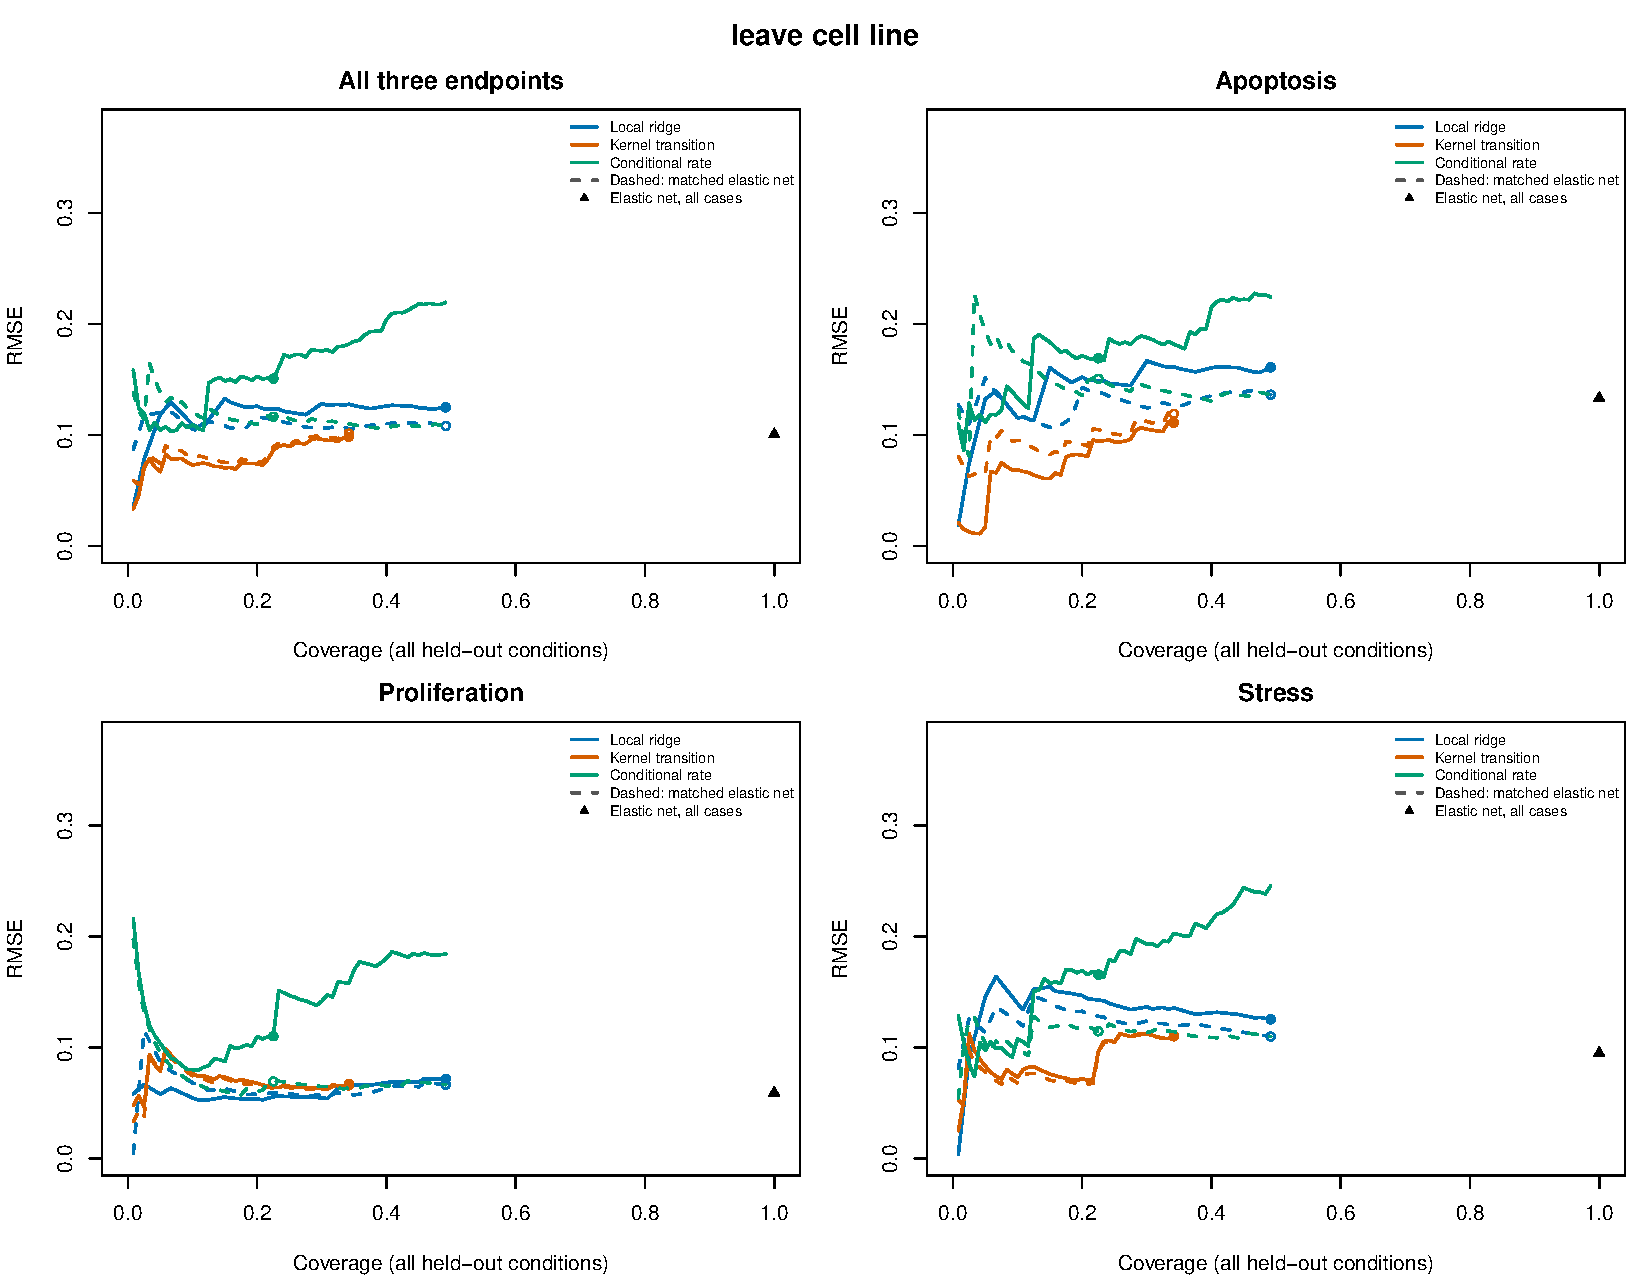
\includegraphics[page=1,width=\textwidth,height=.72\textheight,keepaspectratio]{figure/SuppFigS3_selective_risk_coverage.pdf}
\caption{\textbf{Matched-case selective risk--coverage curves.} Leave cell line. Each response model selects tasks by its uncertainty cutoff after fixed applicability rules. Solid lines show response models; dashed lines in the same colour show elastic net on exactly those selected tasks. The black triangle is full-coverage elastic net. Filled/open circles mark the 0.15 cutoff for the response model/matched comparator. Curves are conditional on frozen out-of-fold predictions and show no unseen-intervention coverage; they are not biological replicate distributions. Each page contains overall, apoptosis-program, proliferation-program and stress-program panels. The next three pages show the other validation axes.}\label{fig:supp-risk}
\end{figure}
\clearpage
\begin{figure}[H]
\centering
\includegraphics[page=2,width=\textwidth,height=.72\textheight,keepaspectratio]{figure/SuppFigS3_selective_risk_coverage.pdf}
\color{black}\par\small\textbf{Supplementary Figure S3, continued.} Leave intervention. Four panels show overall and separate program errors with the same selection and comparator rules. Program-specific vertical scales should be read separately.
\end{figure}
\clearpage
\begin{figure}[H]
\centering
\includegraphics[page=3,width=\textwidth,height=.72\textheight,keepaspectratio]{figure/SuppFigS3_selective_risk_coverage.pdf}
\color{black}\par\small\textbf{Supplementary Figure S3, continued.} Leave source state. Four panels show overall and separate program errors with the same selection and comparator rules. Program-specific vertical scales should be read separately.
\end{figure}
\clearpage
\begin{figure}[H]
\centering
\includegraphics[page=4,width=\textwidth,height=.72\textheight,keepaspectratio]{figure/SuppFigS3_selective_risk_coverage.pdf}
\color{black}\par\small\textbf{Supplementary Figure S3, continued.} Leave target state. Four panels show overall and separate program errors with the same selection and comparator rules. Program-specific vertical scales should be read separately.
\end{figure}

\clearpage
\paragraph{Fully nested baseline-count representation and prediction.}
The additional cell-line evaluation uses the same 21,936 recorded QC-passing baseline cells and all 32,738 measured genes before fold-specific feature selection. Each outer fit removes every cell and context from its held-out lines; each inner fit additionally removes its validation lines. The 128 non-benchmark lines remain an unlabeled reference panel and provide no supervised response examples or applicability neighbours. The 25 fresh training executions cover 15 distinct reference-cell subsets. Symmetric inner fits with identical reference membership gave identical states; these repetitions are not independent biological validation. All fits ran 200 epochs under the recovered settings, with 17,470--20,149 reference cells, 4,000 selected genes, all five batches and no unseen query batch. Query parameters, including batch-normalization state, were unchanged by inference in every fit.

Scaling uses the appropriate supervised training rows. Elastic net retains $\alpha=0.5$; for each endpoint, four grouped inner folds select the minimum pooled validation-MSE penalty from 17 values $10^0,\ldots,10^{-4}$. Latent coordinates from different fits are never pooled into one predictor matrix. For each response model and exploratory RMSE tolerance 0.10, 0.15 or 0.20, inner predictions select the uncertainty cutoff accepting the most supported cases while retaining at least ten cases from three lines. No qualifying cutoff means abstention. All penalties and cutoffs are frozen before evaluating outer errors. The original support, distance, neighbour and 0.15 heuristic rules are retained for the separate fixed-cutoff comparison. This evaluation fixes the original QC cell mask, program definitions and task panel; it does not relearn the entire catalogue or make the original source/target-state axes prospective. Matched-horizon DMSO profiles are observed query inputs, not a demonstrated pretreatment-only policy.

All 75 endpoint-rate-network fits reached the original 600-iteration cap. A fixed 6,000-iteration sensitivity, using the same three initialization seeds, folds and other settings, was specified before examining the new outer performance. All 75 then reported optimizer convergence. It refitted the inner network predictions and cutoffs; non-network predictions, all 15 elastic-net penalties and all 30 non-network cutoffs remained exactly unchanged. Every elastic-net fit completed the full 17-penalty path without an optimization error. Convergence here is an optimizer diagnostic, not proof of a global optimum or validation of a neural ODE.

\paragraph{Supplementary Table S3b. Nested scVI results at the original 0.15 cutoff.}
RMSE averages the three program squared errors before taking the square root. Differences compare each method with elastic net on the identical accepted tasks. Intervals use 2,000 cell-line-cluster bootstrap draws of fixed out-of-fold predictions and decisions; scVI, model fitting and cutoff selection are not repeated. They omit pipeline-training and independent-experiment uncertainty. The 6,000-iteration row changes only the endpoint-rate network's optimizer budget.
\small
\begin{longtable}{p{0.28\textwidth}p{0.10\textwidth}p{0.22\textwidth}p{0.30\textwidth}}
\toprule
\rev{Method} & \rev{Accepted / 120} & \rev{RMSE [95\% interval]} & \rev{Model minus matched elastic net [95\% interval]}\\
\midrule
\endhead
\rev{Training mean} & \rev{120} & \rev{$0.1554$\newline$[0.1165,0.1896]$} & \rev{$0.05690$\newline$[0.02153,0.08909]$}\\
\rev{Static ridge} & \rev{120} & \rev{$0.1214$\newline$[0.1097,0.1323]$} & \rev{$0.02290$\newline$[0.01123,0.03459]$}\\
\rev{Elastic net} & \rev{120} & \rev{$0.0985$\newline$[0.0875,0.1089]$} & \rev{$0.00000$\newline$[0.00000,0.00000]$}\\
\rev{Local response ridge} & \rev{117} & \rev{$0.1062$\newline$[0.0947,0.1166]$} & \rev{$0.00873$\newline$[0.00138,0.01731]$}\\
\rev{Kernel transition} & \rev{96} & \rev{$0.0941$\newline$[0.0801,0.1079]$} & \rev{$-0.00267$\newline$[-0.00580,0.00021]$}\\
\rev{Rate network (600)} & \rev{60} & \rev{$0.3068$\newline$[0.2147,0.3873]$} & \rev{$0.21340$\newline$[0.11499,0.29998]$}\\
\rev{Rate network (6,000)} & \rev{76} & \rev{$0.2553$\newline$[0.2070,0.2985]$} & \rev{$0.16084$\newline$[0.10936,0.20955]$}\\
\bottomrule
\end{longtable}
\normalsize

\clearpage
\paragraph{Supplementary Table S3c. Training-selected cutoffs in the nested scVI evaluation.}
\rev{The inner tolerance is an empirical tuning criterion on the program-tail-fraction RMSE scale.} It is not a guaranteed future-risk bound. Zero coverage is retained as an observed result; ``--'' denotes an undefined error. The complete overall and endpoint-specific metrics, assignments and cutoff values are supplied with the code.
\small
\begin{longtable}{p{0.23\textwidth}p{0.10\textwidth}p{0.08\textwidth}p{0.10\textwidth}p{0.12\textwidth}p{0.25\textwidth}}
\toprule
\rev{Method} & \rev{Inner tolerance} & \rev{Accepted / 120} & \rev{Outer RMSE} & \rev{Matched elastic RMSE} & \rev{Model minus elastic [95\% interval]}\\
\midrule
\endhead
\rev{Local response ridge} & \rev{0.10} & \rev{53} & \rev{0.1099} & \rev{0.0972} & \rev{$0.01262$\newline$[0.00138,0.02508]$}\\
\rev{Local response ridge} & \rev{0.15} & \rev{117} & \rev{0.1062} & \rev{0.0975} & \rev{$0.00873$\newline$[0.00138,0.01731]$}\\
\rev{Local response ridge} & \rev{0.20} & \rev{117} & \rev{0.1062} & \rev{0.0975} & \rev{$0.00873$\newline$[0.00138,0.01731]$}\\
\rev{Kernel transition} & \rev{0.10} & \rev{88} & \rev{0.0903} & \rev{0.0936} & \rev{$-0.00330$\newline$[-0.00660,-0.00037]$}\\
\rev{Kernel transition} & \rev{0.15} & \rev{96} & \rev{0.0941} & \rev{0.0967} & \rev{$-0.00267$\newline$[-0.00580,0.00021]$}\\
\rev{Kernel transition} & \rev{0.20} & \rev{96} & \rev{0.0941} & \rev{0.0967} & \rev{$-0.00267$\newline$[-0.00580,0.00021]$}\\
\rev{Rate network (600)} & \rev{0.10} & \rev{0} & \rev{--} & \rev{--} & \rev{--}\\
\rev{Rate network (600)} & \rev{0.15} & \rev{8} & \rev{0.2034} & \rev{0.1001} & \rev{$0.10330$\newline$[0.03909,0.13302]$}\\
\rev{Rate network (600)} & \rev{0.20} & \rev{43} & \rev{0.3065} & \rev{0.0989} & \rev{$0.20757$\newline$[0.10426,0.30699]$}\\
\rev{Rate network (6,000)} & \rev{0.10} & \rev{8} & \rev{0.1675} & \rev{0.1003} & \rev{$0.06715$\newline$[-0.12952,0.13523]$}\\
\rev{Rate network (6,000)} & \rev{0.15} & \rev{30} & \rev{0.1868} & \rev{0.0975} & \rev{$0.08926$\newline$[0.04017,0.13615]$}\\
\rev{Rate network (6,000)} & \rev{0.20} & \rev{60} & \rev{0.2417} & \rev{0.0941} & \rev{$0.14765$\newline$[0.09051,0.19897]$}\\
\bottomrule
\end{longtable}
\normalsize

\paragraph{Complementary lower-cell-support queries.}
The 41 benchmark lines have 330 original chemical conditions: 120 primary conditions and 210 with fewer than 100 cells in at least one arm (minimum-arm counts 21--99). The latter comprise 144 conditions with the same eight intervention identities, across 31 lines, and 66 with five new identities, across 17 lines. Known-identity deficits are baseline-only in 61 conditions, treated-only in 16 and present in both arms in 67. Each condition joins to its line's outer encoder with exact baseline-cell counts. The 144 known-identity queries use the already fitted primary-panel models, penalties and cutoffs; their outcomes and standard errors are not used in fitting or selection. The 66 novel-identity cases are audited as rejected by the predetermined response identity rule, without assigning them artificial static predictions.

On the 144 known-identity queries, elastic-net RMSE is 0.11990 at full coverage. At the original cutoff, kernel accepts 82/144, with RMSE 0.10330 versus matched elastic net 0.10852; the paired difference is $-0.00522$ [$-0.01019,-0.00023$]. The converged rate network accepts 71/144, with RMSE 0.30060 and a matched difference $+0.19215$ [$0.14260,0.24354$]. Full program-specific, cell-count and probability-SE strata are supplied. Their intervals resample each stratum's observed cell-line clusters, conditional on frozen predictions and decisions. Additional-label reversal leaves primary predictions, penalties, cutoffs and all acceptance decisions unchanged. \rev{These are separate lower-support queries, not additions to the 705-task eligible catalogue.} Differences can reflect both measurement precision and biological/experimental composition; they do not estimate a causal effect of the count gate or generalization to all 1,044 conditions.

\clearpage
\rev{Retrospective intervention choice was evaluated within baseline contexts defined by cell line, experiment and horizon.} \rev{The primary panel contains 57 contexts, of which 30 contain at least two measured drugs.} \rev{Candidate sets required at least two kernel-accepted drugs and were identical for kernel transition and elastic net.} \rev{Apoptosis-associated fractions were maximized and proliferation-associated fractions minimized in separate exploratory objectives.} \rev{Regret was the observed objective gap between the best accepted drug and the prediction-selected drug; all contexts received equal weight.} \rev{Prediction ties were broken by intervention identity without using outcomes.} \rev{The 10,000-draw cell-line-cluster bootstrap retained paired choices and conditioned on fixed out-of-fold predictions, candidate sets and policies.} \rev{The protocol was defined for this exploratory analysis, rather than preregistered before the original study.} \rev{Endpoint estimation, encoder training and threshold selection were not repeated in this bootstrap.}

\rev{\paragraph{Supplementary Table S3d. Retrospective transcriptional intervention choice.}}
\rev{All drug choices concern measured transcriptional fractions, not death, division or treatment benefit.}
\begin{longtable}{p{.17\textwidth}p{.19\textwidth}p{.1\textwidth}p{.17\textwidth}p{.23\textwidth}}
\toprule
\rev{Policy / objective} & \rev{Contexts / candidate tasks} & \rev{Top hits K / E} & \rev{Mean regret K / E} & \rev{Difference K--E [95\% interval]}\\
\midrule
\endhead
\rev{0.15 / apoptosis} & \rev{17 / 62} & \rev{15 / 15} & \rev{0.00421 / 0.00421} & \rev{0; identical choices}\\
\rev{0.15 / proliferation} & \rev{17 / 62} & \rev{6 / 6} & \rev{0.02481 / 0.01959} & \rev{0.00521 [$-0.00717,0.02295$]}\\
\rev{Inner 0.10 / apoptosis} & \rev{16 / 56} & \rev{12 / 14} & \rev{0.01257 / 0.00505} & \rev{0.00751 [$-0.00127,0.02049$]}\\
\rev{Inner 0.10 / proliferation} & \rev{16 / 56} & \rev{7 / 6} & \rev{0.01720 / 0.01951} & \rev{$-0.00231$ [$-0.00958,0.00375$]}\\
\bottomrule
\end{longtable}
\rev{K denotes kernel transition and E denotes elastic net; lower regret is better.} \rev{The original 0.15 cutoff accepts 96 tasks overall, while the exploratory inner tolerance 0.10 accepts 88; only 62 and 56, respectively, enter multi-drug choice contexts.} \rev{Each eligible context has a distinct cell line, yielding 17 or 16 line clusters.} \rev{All choice contexts are at 24 h; 15 are from experiment 3, with the others from experiment 1.} \rev{The inner tolerances 0.15 and 0.20 produce the same choices as the original cutoff.} \rev{Identical empirical decisions yield zero paired regret contrast on these observations, not evidence of known equivalence in future experiments.}

\section*{Supplementary Note S3. Technical non-additivity and combination prediction}

The measured feature set contains 3,591 genes: five names from the nominal 3,596-feature list are absent from the count matrix. Counts are normalized within cells as log1p CP10k, then averaged by simplified condition and technical GEM group. \rev{For matched single-response vectors $d_A,d_B$ and pair response $d_{AB}$, define
{}
{\color{red}
\[
a=d_A+d_B,\quad u=\frac{a}{\max(\lVert a\rVert,10^{-10})},\quad I=d_{AB}-a,\quad s=I^\top u.
\]
}
\rev{}
The pooled singles define $u$ without the observed pair outcome, but they are not independent biological experiments. Eight group-specific projections use matched single and control summaries; a two-sided $t$ test and BH correction across all 131 pairs give a conditional technical test. Classes are assigned in priority order: (1) positive mean projection and $q<0.05$, positive non-additive; (2) negative mean and $q<0.05$, antagonistic; (3) otherwise redundant if $\max[\cos(d_{AB},d_A),\cos(d_{AB},d_B)]>0.8$ and $\lVert d_{AB}\rVert\leq1.1\max(\lVert d_A\rVert,\lVert d_B\rVert)$; (4) otherwise the residual class. The last label does not demonstrate an effect varying across observed biological contexts. None is a therapeutic-synergy claim.}

All 131 pairs enter the descriptive interaction and prediction analysis. The 269-task Norman catalogue instead includes 152 singles and 117 pairs with at least 100 cells; the other fourteen pairs have 51--96 cells. Eight GEM groups are lanes/technical partitions of one pooled experiment (GSM3906024), so confidence intervals, exact sign flips, bootstrap checks and held-out-GEM directions all remain within that experiment. They do not establish independent biological replication.

Exact reaggregation reproduces all primary effects, intervals, FDRs and labels within $10^{-10}$. Log1p CPM gives ten positives, 113/131 unchanged labels and seven of eight retained primary positives. Gene-SD-scaled CP10k gives two positives, 98/131 unchanged and two of eight retained positives. Recomputing the target direction from singles in the other seven GEM groups gives fifteen positives, retaining all eight primary positives. All eight have positive lower technical-bootstrap bounds and positive leave-one-GEM-out mean projections. \rev{The exact $2^8$ sign-flip diagnostic retains seven after BH correction; TGFBR2--C19orf26 has $q=0.05182$.} These differences show representation and orientation sensitivity.

Positive counts across increasing summed-single-norm quartiles are 4/33, 2/33, 2/32 and 0/33; across increasing projection-SE quartiles they are 2/33, 3/33, 3/32 and 0/33. Summed magnitude and projection SE are correlated (Spearman $0.492$). Thus effect scale and estimation precision contribute to classification. The sensitivity tables retain all 131 pairs, their constituent genes and exact statistics.

\paragraph{Supplementary Table S4. The eight primary positive pairs.}
The projection means, intervals and $q$ values concern technical variation within one pooled experiment. The final column is the alternative exact sign-flip $q$, not an independent biological confirmation.
\begin{longtable}{p{0.32\textwidth}p{0.09\textwidth}p{0.29\textwidth}p{0.1\textwidth}p{0.12\textwidth}}
\toprule
\rev{Pair} & \rev{$n_{cells}$} & \rev{Mean [95\% $t$ interval]} & \rev{BH $q$} & \rev{Sign-flip $q$}\\
\midrule
\endhead
\rev{CBL--UBASH3B} & \rev{373} & \rev{1.237 [0.702, 1.771]} & \rev{0.00231} & \rev{0.016}\\
\rev{CNN1--UBASH3A} & \rev{165} & \rev{2.328 [1.568, 3.089]} & \rev{0.00059} & \rev{0.016}\\
\rev{DUSP9--SNAI1} & \rev{175} & \rev{1.410 [0.534, 2.285]} & \rev{0.0134} & \rev{0.016}\\
\rev{FEV--CBFA2T3} & \rev{149} & \rev{3.243 [2.697, 3.789]} & \rev{2.05e-05} & \rev{0.016}\\
\rev{FEV--ISL2} & \rev{275} & \rev{1.413 [0.944, 1.883]} & \rev{0.000641} & \rev{0.016}\\
\rev{PTPN12--UBASH3A} & \rev{290} & \rev{1.275 [0.325, 2.224]} & \rev{0.028} & \rev{0.0399}\\
\rev{TGFBR2--C19orf26} & \rev{308} & \rev{0.548 [0.148, 0.948]} & \rev{0.026} & \rev{0.0518}\\
\rev{UBASH3B--CNN1} & \rev{386} & \rev{1.218 [0.601, 1.834]} & \rev{0.00507} & \rev{0.0288}\\
\bottomrule
\end{longtable}
\paragraph{Generalization task and intervals.}
Measured single responses for test genes remain available; held-out combinations, not uncharacterized genes, are predicted. Primary Pfam assignment selects the domain represented by the largest number of assayed genes and breaks ties lexicographically. There are 69 annotated and four unannotated genes. Only primary families with at least three pairs supply test anchors. Genes in the held-out primary family are removed from training; secondary shared domains are not all excluded. An unannotated gene can enter a test pair through its annotated partner; one pair has no eligible family anchor (130 family-test pairs).

Positive prevalence is 8/131 (6.11\%) for leave-gene and 8/130 (6.15\%) for leave-family. Two of five gene folds and fifteen of 22 family folds contain no positives; per-fold AUROC is undefined there. Fixed out-of-fold predictions are resampled 2,000 times by anchor gene (65 blocks) or primary family (22 blocks). These conditional intervals do not eliminate dependence from shared partner genes or quantify independent biological replication. Draws lacking both outcome classes are excluded for AUROC, with valid counts retained in the output.

For XGBoost, leave-gene AUROC is 0.687 [0.499, 0.828], average precision 0.108 [0.044, 0.269], RMSE 1.578 [1.335, 1.824], and Spearman correlation 0.507 [0.322, 0.650]. Leave-family values are 0.788 [0.655, 0.902], 0.154 [0.073, 0.351], 1.631 [1.367, 1.896], and 0.459 [0.275, 0.636], respectively. Single-response magnitude gives average precision 0.150 and 0.160. \rev{All-model intervals and per-fold class counts are supplied; the eight positives do not justify a general positive non-additivity prediction claim.}

\paragraph{Paired baseline comparison and label sensitivity.}
Using identical sampled anchor-gene (65 blocks) or primary-family (22 blocks) indices for each method, 2,000 conditional bootstrap draws compare XGBoost with summed-single-response magnitude. XGBoost-minus-baseline AUROC differences are $-0.0183$ [$-0.1174,0.1039$] and $0.0574$ [$-0.0546,0.1671$]; average-precision differences are $-0.0411$ [$-0.2811,0.0251$] and $-0.00615$ [$-0.1471,0.0976$]. Interaction-RMSE differences are $0.0974$ [$-0.0854,0.3301$] and $0.1159$ [$-0.0158,0.2465$]. These paired intervals do not establish incremental performance. Shared partner genes and the single pooled experiment remain dependence limits.

Without retraining scores, XGBoost AUROCs under leave-gene / leave-family validation are 0.612/0.693 against log-CPM labels (ten positives), 0.717/0.672 against gene-SD-scaled labels (two positives), and 0.645/0.765 against exact technical-sign-flip labels (seven positives), compared with primary 0.687/0.788. The two-positive definition yields average precision only 0.0385/0.0494. Valid bootstrap counts are supplied where draws lack positives. These are frozen-score label sensitivities, not newly trained alternative-label prediction models.

\paragraph{Orthogonal bulk-growth correspondence.}
Exact selected CRISPRa guides and the authors' label mappings link the RNA conditions to the original two filter15 bulk-growth maps. These measure ten-day guide-pair enrichment relative to negative controls, normalized by source-reported population doublings, separately from the single-cell transcriptomes; construct orientations are averaged. The normalized growth phenotype is not a transcriptional score or genetic-interaction residual. Both growth replicates are finite for 121/131 pairs, including 110/117 eligible pair tasks across 15/16 basins. One pair lacks the selected SLC38A2 guide; nine others use FEV/CEBPA guides absent from the filtered growth maps. Missing values are not imputed. Per-basin support is 1--21 pairs, with one singleton; complete guide mapping, missingness and basin summaries are supplied.

The descriptive between-basin fraction of observed growth variation is $\eta^2=0.7423$ for the replicate mean and 0.7329/0.7339 for the separate replicates. Here $\eta^2$ is the between-group sum of squares divided by the total sum of squares, not cross-validated prediction accuracy. Replicate Pearson correlation is 0.956 among the 110 matched eligible pairs. Median absolute growth difference is 0.0841 within and 0.1918 between basins, from 583 and 5,412 dependent comparisons. No inferential $P$ value or biological-replicate interval is assigned: pairs share genes and pairwise distances reuse conditions, while RNA combinations were selected from the growth GI map. This supplies a functional correspondence in an ascertained panel from the same source study, without establishing stable fates, trajectories, alternative biological routes or an additional biological context for control-node assessment.

\paragraph{\rev{Exploratory endpoint-graph summaries.}}

To describe similarities among endpoints measured under different perturbation sets, we grouped eligible Norman conditions into response basins. Mean silhouette across $k=8,\ldots,24$ selected $k=18$; 16 basins contained eligible pairs. Within each basin, observed pairs were linked when endpoint-response cosine exceeded 0.80. \rev{We summarized the effective number of connected response components and the similarity between endpoints produced by disjoint gene sets (Supplementary Fig.~\ref{fig:paths}).} \rev{At the primary threshold, ten basins had effective component diversity below two, whereas three had diversity of at least four.}

\begin{figure}[H]
\centering
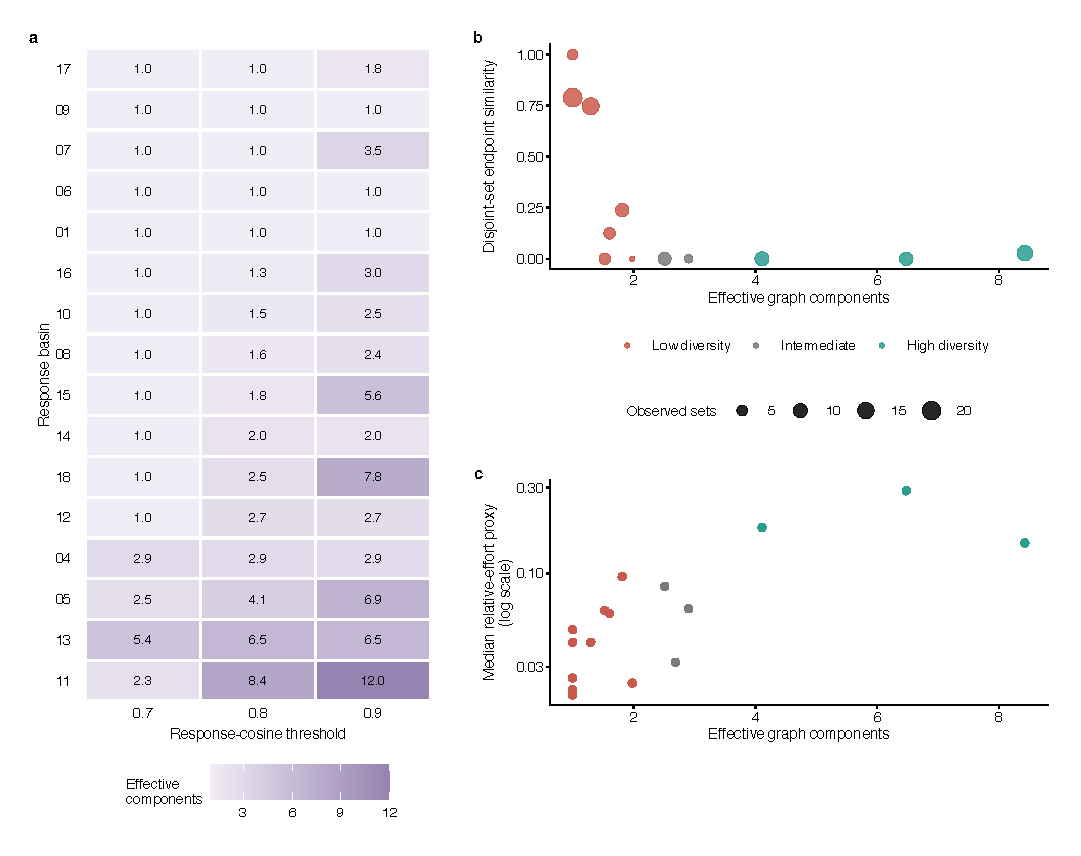
\includegraphics[width=\textwidth]{figure/Fig6_control_degeneracy.pdf}
\caption{\rev{\textbf{Endpoint-graph diversity depends on basin and similarity threshold.} \textbf{a}, Effective component counts for 16 response basins at cosine thresholds of 0.70, 0.80 and 0.90, ordered at 0.80.} \rev{\textbf{b}, Effective component count versus disjoint-set endpoint similarity at 0.80; point size denotes observed control-set count.} Four basins lacked evaluable comparisons. \textbf{c}, Diversity versus median intervention-based relative effort on a logarithmic axis. Relative effort is intervention size divided by squared endpoint-response magnitude, an empirical ranking rather than physical control energy. Colours denote low ($<2$), intermediate or high ($\geq4$) diversity. These measures do not establish pathway substitutability.}
\label{fig:paths}
\end{figure}

The designation was not invariant to the graph threshold. Cosine thresholds of 0.70, 0.80 and 0.90 produced 12, 10 and five low-diversity basins, respectively, and one, three and five high-diversity basins. \rev{Values displayed in Supplementary Fig.~\ref{fig:paths}a are rounded to one decimal place; diversity classifications and basin counts use unrounded values.} \rev{Median relative-effort proxy also did not decrease monotonically with component diversity.} \rev{We therefore interpret endpoint-graph diversity solely as an endpoint-similarity graph statistic.} The growth correspondence below does not validate these basins as stable cellular fates or graph components as actual routes through state space. Simultaneous pairs do not identify an intervention order, and basins learned from the same endpoint space are descriptive response classes rather than independently established biological fates.

A separate bulk-growth assay from the source study matched 110 of 117 eligible pairs across 15 of 16 basins. Growth differed descriptively across basins ($\eta^2=0.742$), and absolute differences were smaller within than between basins (medians 0.084 and 0.192). The RNA combinations had been selected from that growth-interaction screen and pairs share genes, so this is an orthogonal phenotype association within an ascertained panel, not unselected external validation. \rev{It links the RNA grouping to relative growth without establishing stable fate identity or biological routes.}



\section*{Supplementary Note S4. Multiome agreement and gene-evidence coverage}

MultiPerturb RNA guide-pseudobulk counts and gene-linked ATAC counts are normalized as log1p CPM. ATAC peak assignment uses only deposited nonempty \texttt{gene\_symbol} annotations; counts of all peaks assigned to a gene are summed. No new proximity or correlation-based peak links are inferred. The supplied annotation is preserved. TSS-window restrictions are tested below; new peak-link inference was not performed. The top 2,000 variable RNA and ATAC response features define the frozen modality summaries.

\rev{All 99 target--context rows are ATRT human targets; mouse cells in the deposited object are non-targeting controls.} \rev{Count, guide and nuisance rules retain 27 targets, of which ten pass joint median RNA--ATAC cosine cutoffs above 0.10.} \rev{The ten agreement-selected targets have 24 guides, 138--2,139 cells per target and at least 15 cells per guide.} \rev{The 0.10 rule is descriptive and does not discriminate target responses from non-targeting control variation.} \rev{No modality role is assigned from these agreement scores.}

\rev{A separate 999-draw same-context random-guide-group null preserves each target's guide count.} \rev{Its minimum nominal $P$ is 0.019 (BH $q=0.2565$ across 27 targets).} \rev{This unrelated-guide-group diagnostic differs from the non-targeting-construct test below and is not used to retain targets.} \rev{Among the 24 agreement-selected guides, RNA movement versus cell count has Spearman $\rho=-0.941$, ATAC movement versus cell count $-0.854$, and ATAC movement versus mean library size $-0.750$.} \rev{These correlations do not identify a technical cause, but show that the original nuisance rule did not isolate abundance-independent movement.}

\paragraph{Count-based, annotation and negative-control checks.}
The compact source-derived input retains 51,829 necessary cells from the 27 supported targets (64 guides) and ten human non-targeting guides, with original 2,000-feature RNA and gene-linked ATAC counts, library totals, target-RNA counts and alternative TSS aggregates. The original deposited object independently reconstructed the primary features and guide summaries. \rev{Restricting deposited peak annotations to within 2 kb (1,832 covered genes) or 10 kb (1,915) of the annotated TSS retains the ten agreement-selected targets and adds one.} \rev{This preserves descriptive agreement rather than validating a target-specific modality role.} Original count/guide/nuisance gates remain fixed. This tests annotation-window sensitivity, not newly inferred or experimentally validated peak links.

For a genuine non-targeting construct null, all 36 two-guide and 84 three-guide groups from the nine sufficiently populated human control guides are evaluated against the remaining control guides, excluding each tested group from its reference. Their 95th-percentile joint cosines are 0.427 and 0.440, and 38.9\%/65.5\% exceed both 0.10 cutoffs. These overlapping construct groups are not independent biological replicates. \rev{No supported target passes BH $q<0.05$ across 27 tests (minimum adjusted $q=0.6353$).} A separate 999-draw guide-label diagnostic matches cell abundance, library depth and response amplitude; it remains a specificity sensitivity, not a new biological experiment.

Equal-cell sampling uses 100 draws without replacement at 15, 30 and 50 cells per guide. With a shared anchor constructed by the original cell-weighted rule from the nine adequately populated control guides, median passing counts become 27, 26 and 25; however, nearly all similarly sampled non-targeting groups also pass. This is not evidence of improved reproducibility: shared reference error and unequal-depth log transformations can create common response components. A complementary diagnostic gives every guide a distinct non-targeting reference with the same cell count and a closely matched library total, using 199 pooled-cell null draws per guide-count/depth stratum and 50 target draws. At these depths, no target passes both 0.10 thresholds in any draw, while control-null 95th percentiles are 0.016--0.023. Independent-reference sampling also removes the shared reference component and reduces support; it is a different diagnostic, not a replacement primary test. Both analyses are retained. Their disagreement demonstrates reference/depth sensitivity and does not establish that the biological perturbations have no effect.

Target-RNA depletion compares guide-pseudobulk target counts per RNA library with human non-targeting cells, with 0.5-count and one-library-unit pseudocounts. Control target counts of at least 20 make 17 of the 24 primary guides estimable; 12 have lower point estimates and only two have a pointwise 95\% cell-bootstrap upper bound below zero (500 draws). Intervals describe cell sampling within constructs and are not multiplicity-corrected independent-guide confirmation. Median estimable log2 ratio is $-0.537$; correlations with RNA and ATAC movement are 0.179 and 0.191. This is an on-target transcript proxy, not direct editing, chromatin recruitment or guide-efficiency measurement.

\paragraph{Gene universes and criterion availability.}

\rev{The following counts use only the apoptosis/proliferation/stress and multiome endpoint definitions of this assay-specific catalogue.} \rev{RPE1 UPR responses use separate readouts and support criteria, so these coverage counts do not describe the harmonized analysis populations in the main text.}
The union contains 9,894 targeted symbols: 9,867 in the genome-wide breadth screen plus 27 additional symbols. \rev{Within each breadth-screen gene, the minimum transcript-level energy-test $P$ is multiplied by the number of transcript tests, capped at one, then BH-adjusted across genes.} \rev{A gene below $q=0.05$ is a state marker only if it has no higher evidence class; this is an association criterion rather than a marker-specificity assay.} \rev{After requiring the MultiPerturb non-targeting-construct test, the classes contain 389 perturbation-supported genes, 4,128 state markers and 5,377 genes with insufficient perturbation evidence.} \rev{The agreement-only comparison gives 398, 4,122 and 5,374; nine MultiPerturb-only assignments account for the shift.}

\rev{Twenty-seven genes have cell-level assays in both K562 and ATRT, but none has an observed Norman combination.} \rev{Thus the available assay overlap prevents complete control-node assessment for every gene.} \rev{PRMT5 had movement support in both contexts under agreement-only rules, but its ATRT evidence fails the non-targeting-construct test.} \rev{Combination assays are available for 73 genes, of which six meet the original consistency rule and 67 do not; 9,821 lack pair measurements.} \rev{The K562 specificity contrast is evaluable for 389 genes, with 237 meeting its numerical rule and 152 not meeting it.} \rev{CRISPRi and CRISPRa evidence remains source-resolved, and repeated K562 resources count as one context.}

\rev{The source-specific filters use Replogle off-target-deviation quantiles or Norman agreement and the balance of observed positive versus antagonistic combinations.} \rev{These are operational contrasts, not a target-specific competition among all available interventions.} \rev{Threshold changes cannot repair the absence of overlapping assays.} \rev{The gene table therefore records assay availability and numerical rule status without assigning a validated candidate priority.} \rev{The retained task catalogue contains 705 rather than the agreement-only 715 tasks, with non-MultiPerturb sources unchanged.}

The experimental roadmap is evidence-specific: a marker needs a controlled perturbation and matched functional endpoint; a one-context regulator needs replication in a distinct biological context; a gene without combination evidence needs a measured combination with matched singles; target specificity requires comparison with competing interventions and non-target phenotypes; stable control requires held-out contexts, longitudinal attainment and post-withdrawal persistence. None of these missing experiments is claimed as completed.

\section*{Supplementary Note S5. Duration contrasts under continued exposure}

The duration analysis starts from the 1,115 source pairs (minimum 20 cells per arm), not only the 151 tasks satisfying the 100-cell gate. \rev{The increase/nonincrease classification uses both observed endpoints:
{}
{\color{red}
\[
\mathrm{SE}_{6h}\leq0.10\;\text{and}\;\mathrm{SE}_{24h}\leq0.10\;\text{and}\;\max_j p_{j,24h}>\max_j p_{j,6h}.
\]
}
\rev{}
All 158 matched contexts meet both SE criteria, so 101/57 is entirely the positive/nonpositive maximum-change split. Different cells are sampled at the two exposure durations. The maximizing program changes in 71 contexts. Fixing the target to the 6-h maximizing program gives an increase in 68/158, rather than 101/158. This fixed-target analysis is itself retrospective, not a preregistered policy test.}

\paragraph{Supplementary Table S5. Drug-level descriptive contrasts.}
\begin{longtable}{p{0.2\textwidth}p{0.06\textwidth}p{0.23\textwidth}p{0.23\textwidth}p{0.18\textwidth}}
\toprule
\rev{Drug} & \rev{$n$} & \rev{Separate maxima increase} & \rev{Fixed 6-h target increase} & \rev{Maximizer changes}\\
\midrule
\endhead
\rev{BRD3379} & \rev{88} & \rev{68} & \rev{44} & \rev{49}\\
\rev{Bortezomib} & \rev{22} & \rev{9} & \rev{9} & \rev{0}\\
\rev{Idasanutlin} & \rev{24} & \rev{11} & \rev{9} & \rev{9}\\
\rev{Trametinib} & \rev{24} & \rev{13} & \rev{6} & \rev{13}\\
\bottomrule
\end{longtable}
These drug differences are confounded by sampled cell lines and experiment; no mechanism-of-action contrast was tested. There is no stopping/washout comparator. Therefore the data describe endpoints during continued exposure and do not estimate continuation benefit or validate an adaptive policy. A policy test would require a specified target, decision variables available before the intervention, stopping/switching comparators and longitudinal or functional validation of attainment and persistence.

\begin{figure}[H]
\centering
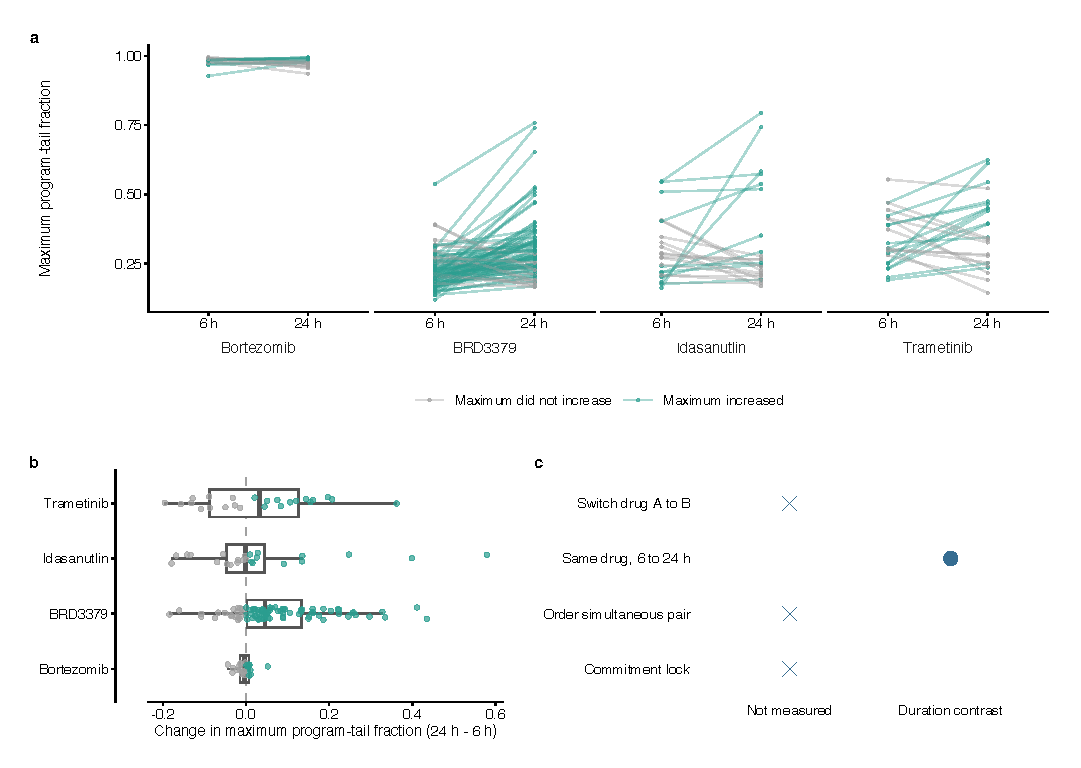
\includegraphics[width=\textwidth]{figure/Fig7_observed_support_sequences.pdf}
\caption{\rev{\textbf{Population endpoints under matched exposure durations.} \textbf{a}, Paired maximum transcriptional-program tail fractions at 6 and 24 h for 158 matched drug--cell-line contexts, stratified by drug.} Lines connect context-level endpoints, not longitudinally tracked individual cells. The maximizing program can differ between endpoints. \rev{Colour identifies the observed increase (101 contexts) or nonincrease (57) in the maximum tail fraction; neither represents a prospective continuation decision.} \rev{\textbf{b}, Within-context change in the maximum tail fraction; dots denote contexts, boxes show median and interquartile range, and whiskers extend to observations within 1.5 interquartile ranges.} \textbf{c}, Evidence boundary: same-drug exposure durations were compared; unobserved switches, pair order and commitment locks were not evaluated.}
\label{fig:sequence}
\end{figure}




\paragraph{Reproducibility scope.}
\rev{Separate numerical implementations reconstructed the 131 Norman interaction classes and the nested-prediction endpoint errors from preserved processed inputs.} \rev{All Norman labels agreed, with maximum projection and interval discrepancy $5.33\times10^{-15}$.} \rev{This verifies selected calculations from processed profiles rather than independently validating upstream QC, biological interpretation or new experiments.} MultiPerturb and RNA-baseline extraction, nested count-level scVI training and both optimization budgets were executed; baseline counts were reconstructed from five checksum-verified archives. Network re-downloading, raw-read processing, original QC/endpoint reconstruction, new peak-link inference, independent biological replication and prospective policy experiments were not performed. \rev{Source-analysis code, processed data, versions, seeds and test records are available at \url{https://github.com/azusakou/State-dependent-response-geometry}.} \rev{Additional simulation and intervention-choice scripts and prepared inputs are provided in the accompanying reproducibility archive, with task-level results in the Supplementary Data.}

\section*{\rev{Supplementary Note S6. Controlled lineage-sampling simulation}}

\rev{For clone $j$ in future condition $c$, intrinsic branch probabilities were $\operatorname{softmax}(\log\pi_c+\sigma z_j)$, with a standard-normal branch vector $z_j$ shared across that clone's recorded conditions.} \rev{The condition offsets $\pi_c$ were descendant-weighted observed branch frequencies with a half-count pseudocount for every branch.} \rev{They calibrate composition and do not estimate the actual unobserved probabilities of individual clones.} \rev{The latent model imposes no stress or baseline-neighbourhood dependence.} \rev{For each resource and $\sigma\in\{0.5,1,2\}$, 200 latent draws were reused across nine observation scenarios.} \rev{These are 1,200 latent-draw datasets and 10,800 scenario records, not 10,800 independent replicates.}

\rev{Matched scenarios observed the same probabilities at recorded descendant counts, ten descendants per existing row, or counts permuted within future condition.} \rev{Random-donor scenarios preserved future condition, neighbourhood size and exclusion of the query.} \rev{A separate analysis selected the actual at-least-ten-descendant populations (92 cytokine and 284 in vitro units) and rebuilt PCA and neighbours.} \rev{Each design retained its original regression covariates, including recorded log descendant count in equal-depth scenarios, to isolate measurement changes from adjustment changes.} \rev{Effective rank used the manuscript eigenvalue-entropy definition, assigning zero rank to exact-zero covariance.} \rev{Separate R and Python implementations reconstructed the archived ranks within $10^{-8}$ and the adjusted stress slopes $-0.0926340$ and $-0.3399896$.}

\rev{At $\sigma=1$, median neighbourhood rank changed from 2.629 to 3.018 in the cytokine design and from 2.981 to 3.573 in vitro under recorded-depth sampling.} \rev{The paired sampling-minus-intrinsic stress-coefficient changes had medians $+0.0171$ and $+0.0137$, with 95\% simulation ranges $[-0.0727,0.0827]$ and $[-0.1324,0.1716]$.} \rev{Equalizing to ten descendants narrowed these ranges to $[-0.0409,0.0398]$ and $[-0.0611,0.0721]$.} \rev{For intrinsic probabilities alone, restricting to deep clones widened the stress-coefficient ranges from $[-0.0475,0.0518]$ to $[-0.0770,0.0813]$ in cytokine and from $[-0.0693,0.0639]$ to $[-0.1100,0.1175]$ in vitro.} \rev{All dispersion and observation settings are provided in the machine-readable supplementary data.}

\rev{These computational ranges are not biological confidence intervals or formal tests against the observed stress coefficients.} \rev{The simplified null does not reproduce a systematic negative sampling bias and cannot determine the latent probabilities in the observed data.} \rev{It separates measurement and population-support effects without providing independent biological replication or explaining the observed sign reversal.}

\begin{figure}[H]
\centering
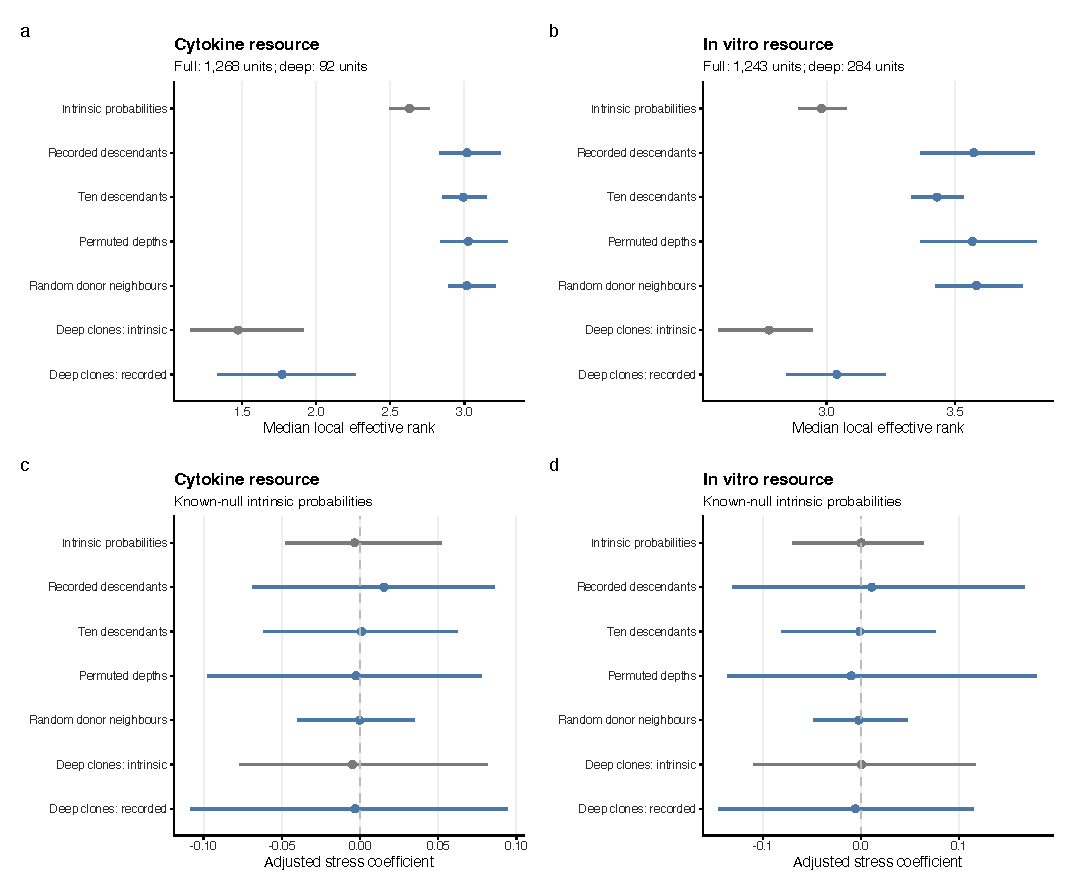
\includegraphics[width=\textwidth]{figure/SuppFigS6_lineage_sampling_null.pdf}
\caption{\rev{\textbf{Descendant sampling changes local covariance geometry under a stress-independent probability model.} \textbf{a,b}, Median neighbourhood effective rank in the cytokine and in vitro designs.} \rev{\textbf{c,d}, Adjusted stress coefficients in the corresponding designs.} \rev{Dots show medians across 200 independently simulated datasets; horizontal lines span the 2.5th--97.5th simulation percentiles, not biological confidence intervals.} \rev{Grey denotes intrinsic clone probabilities and blue denotes multinomially sampled descendant fractions.} \rev{The same latent draw is reused across observation scenarios.} \rev{Full designs contain 1,268 and 1,243 clone--condition units; deep designs retain 92 and 284 units with rebuilt neighbourhoods.} \rev{Displayed results use latent logit standard deviation 1; values 0.5 and 2 are also evaluated.} \rev{Random donor neighbourhoods preserve future condition, neighbourhood size and exclusion of the query.} \rev{The latent model imposes no stress or baseline-neighbourhood dependence; these controls are not independent lineage experiments.}}
\label{fig:supp-simulation}
\end{figure}


\clearpage
\section*{\rev{Supplementary Note S7. Assay-specific supporting results}}

\rev{These supporting analyses use assay-specific catalogue and endpoint definitions.} \rev{Their task eligibility and evidence classes are distinct from the outcome-independent harmonized panels in the main text and Notes S8--S11.}

\subsection*{Stress--geometry associations depend on descendant support}
\begin{figure}[tbp]
\centering
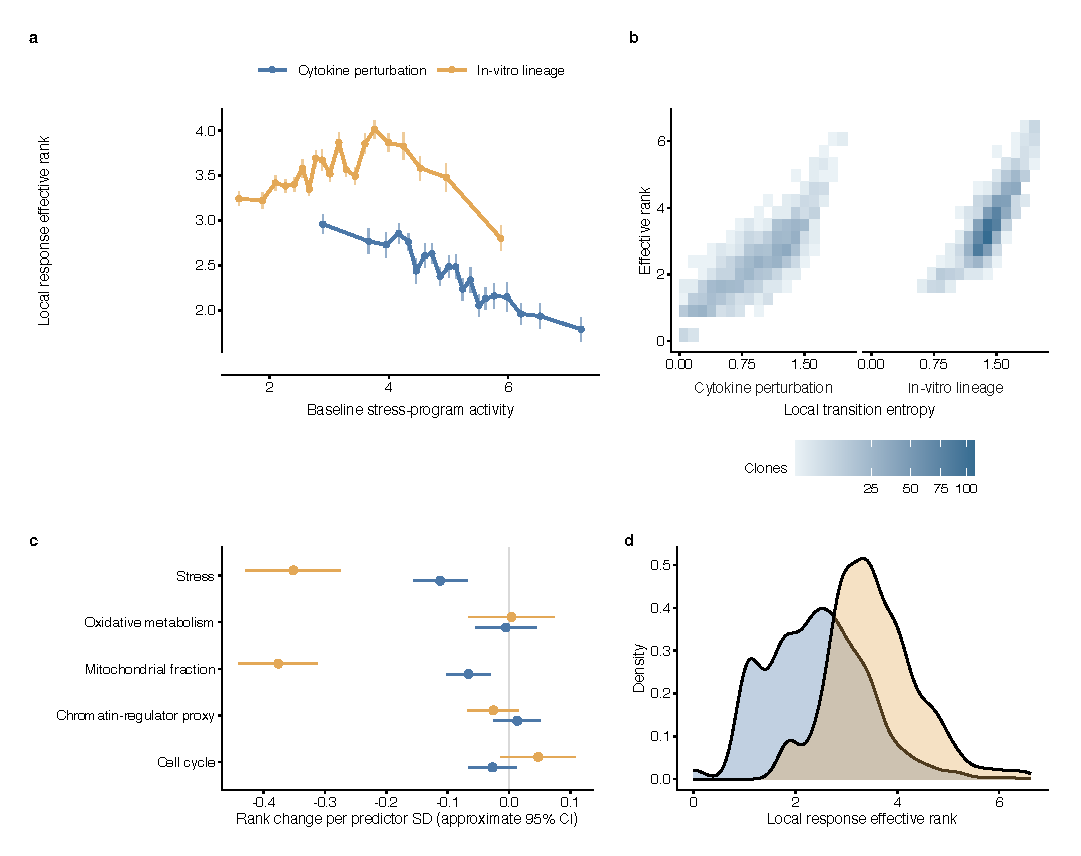
\includegraphics[width=\textwidth]{figure/Fig2_local_controllability.pdf}
\caption{\rev{\textbf{Baseline state and observed local lineage-response geometry.} \textbf{a}, Mean local response effective rank across 20 within-dataset stress bins; bars, one standard error across equally weighted clones.} \textbf{b}, Joint distributions of transition entropy and effective rank; shading denotes clone counts. \textbf{c}, Adjusted rank change per within-dataset predictor standard deviation; bars, estimate $\pm1.96$ standard errors, not permutation confidence intervals. Tested axes were excluded from their own neighbourhood construction; inferential $P$ values reported in the text use 999 clone-level partial-residual permutations. \textbf{d}, Clone-level effective-rank densities. The cytokine and in vitro resources contribute 1,065 and 1,243 clones, respectively.}
\label{fig:local}
\end{figure}
We next tested whether baseline state was associated with local variation among observed descendant-probability vectors. For each LARRY future condition, day-2 cells were aggregated by clone and embedded in baseline pathway--regulon space. We then calculated, among neighbouring baseline clones, the covariance of descendant branch probabilities (Supplementary Fig.~\ref{fig:local}). The entropy-based effective rank of this covariance measures how many outcome directions carry appreciable local variation: high rank denotes variation along several probability-space axes, whereas low rank denotes concentration of variation along fewer axes. Several fates can retain substantial probability even at low rank; rank is not a count of reachable fates. This quantity describes observed lineage-response geometry and is not a gene-level Kalman controllability rank.

With all baseline features, the cytokine resource contained 1,268 unique clone--future-condition units from 1,065 clones and had a median effective rank of 2.44. The in vitro differentiation resource contained 1,243 clone units and had a median rank of 3.42. Both had a median of seven branches with mean local probability below 0.05. These unsupported branches are locally rare outcomes, rather than mathematically unreachable states, because finite sampling cannot distinguish zero probability from a sufficiently small probability.

Inference used clone, not clone--condition row, as the independent biological unit. To avoid circularity, each tested state feature was excluded from the neighbourhood representation used to construct its own local geometry. Models adjusted for future condition when more than one condition was present. With 999 clone-level partial-residual permutations, higher baseline stress was associated with lower effective rank in both datasets: the cytokine coefficient was $-0.109$ (empirical $P=0.001$, Benjamini--Hochberg-adjusted $P=0.005$), and the in vitro coefficient was $-0.327$ (empirical $P=0.001$, adjusted $P=0.0025$). Mitochondrial fraction was also negative in both resources (coefficients $-5.73$ and $-14.76$ per unit fraction on a 0--1 scale, equivalent to $-0.0573$ and $-0.1476$ per percentage point; adjusted $P=0.005$ and $0.0025$, respectively). \rev{Supplementary Fig.~\ref{fig:local}c instead multiplies each raw coefficient by that predictor's within-resource standard deviation across unique clones.} Chromatin-regulator, cell-cycle and oxidative-metabolism scores did not survive correction.

\rev{Adjustment for baseline and descendant cell counts, detected-gene complexity and baseline library identity retained the original stress-specific geometry in the five-state model.} Stress coefficients remained negative ($-0.0926$ and $-0.3400$); 200 clone-cluster bootstrap draws that recomputed principal components, neighbours and covariance gave 95\% percentile intervals of $[-0.203,-0.0457]$ and $[-0.418,-0.179]$. All 12 neighbourhood, representation, principal-component and covariance-shrinkage settings retained negative point estimates. However, sampling sensitivity was substantial: rarefaction to ten descendants retained only 92 of 1,268 cytokine units and reversed the median coefficient to $+0.0412$, whereas the in vitro median remained negative ($-0.0851$). At two or five descendants, all 100 rarefactions per resource had negative coefficients. These results support a conditional association, not a sampling-invariant biological restriction (Supplementary Note S1; Supplementary Fig.~S2).

After balancing measured quality and abundance, high-minus-low stress differences in rank were $-0.168$ (95\% conditional clone-bootstrap interval $[-0.250,-0.087]$) for cytokine and $-0.073$ ($[-0.186,0.030]$) in vitro. Adding other state scores gave $-0.135$ ($[-0.212,-0.052]$) and $-0.089$ ($[-0.209,0.023]$). These overlap-population contrasts differ from continuous stress slopes and condition on the original geometry. The in vitro contrast was uncertain and had limited common support. Selecting the strict high-depth cytokine queries reversed the slope even with their original ranks fixed, implicating population selection as well as altered local resolution (Supplementary Note S1).

\rev{Simulation separated intrinsic branch-probability covariance from descendant sampling while retaining the recorded baseline design.} \rev{Under stress-independent intrinsic probabilities, recorded-depth sampling increased median local rank from 2.63 to 3.02 in the cytokine design and from 2.98 to 3.57 in vitro (latent logit standard deviation 1; 200 simulated datasets per design).} \rev{Sampling changed adjusted stress coefficients across realizations, and selecting deeply sampled clones widened their distribution even for intrinsic probabilities (Supplementary Fig.~S6).} \rev{The simulation did not reproduce a systematic negative stress coefficient; it establishes measurement sensitivity rather than biological validation of the observed association.}

The original stress and mitochondrial coefficients had concordant signs across the two arms of the same study; this is not independent biological replication of a fate map. Models trained on shared baseline axes transferred differentiation propensity only modestly between resources (Spearman $\rho=0.324$ and $0.283$). Transfer was weaker for transition entropy and rare-fate probability ($\rho=0.023$--$0.098$). These transfer results show limited portability across the sampled settings. They do not isolate a causal effect of environment on global fate topology or show that baseline stress sets a biological boundary.



\subsection*{Predictive utility depends on the held-out axis and abstention coverage}

In the frozen-representation benchmark, we modeled MIX-Seq transcriptional-program tail fractions using a training mean, static ridge, elastic net and three response-aware proxies (Supplementary Fig.~\ref{fig:models}). The local-response ridge estimated a neighbourhood-weighted linear map. The kernel-transition model averaged responses among supported nearby source states, prioritizing matching interventions. The conditional-rate network converted endpoint tail fractions into a constant logit-rate relative to a fixed 0.1 prior. Because MIX-Seq contains sparse endpoints rather than dense trajectories, the conditional-rate network was not interpreted as an identified neural ordinary differential equation.
\begin{figure}[tbp]
\centering
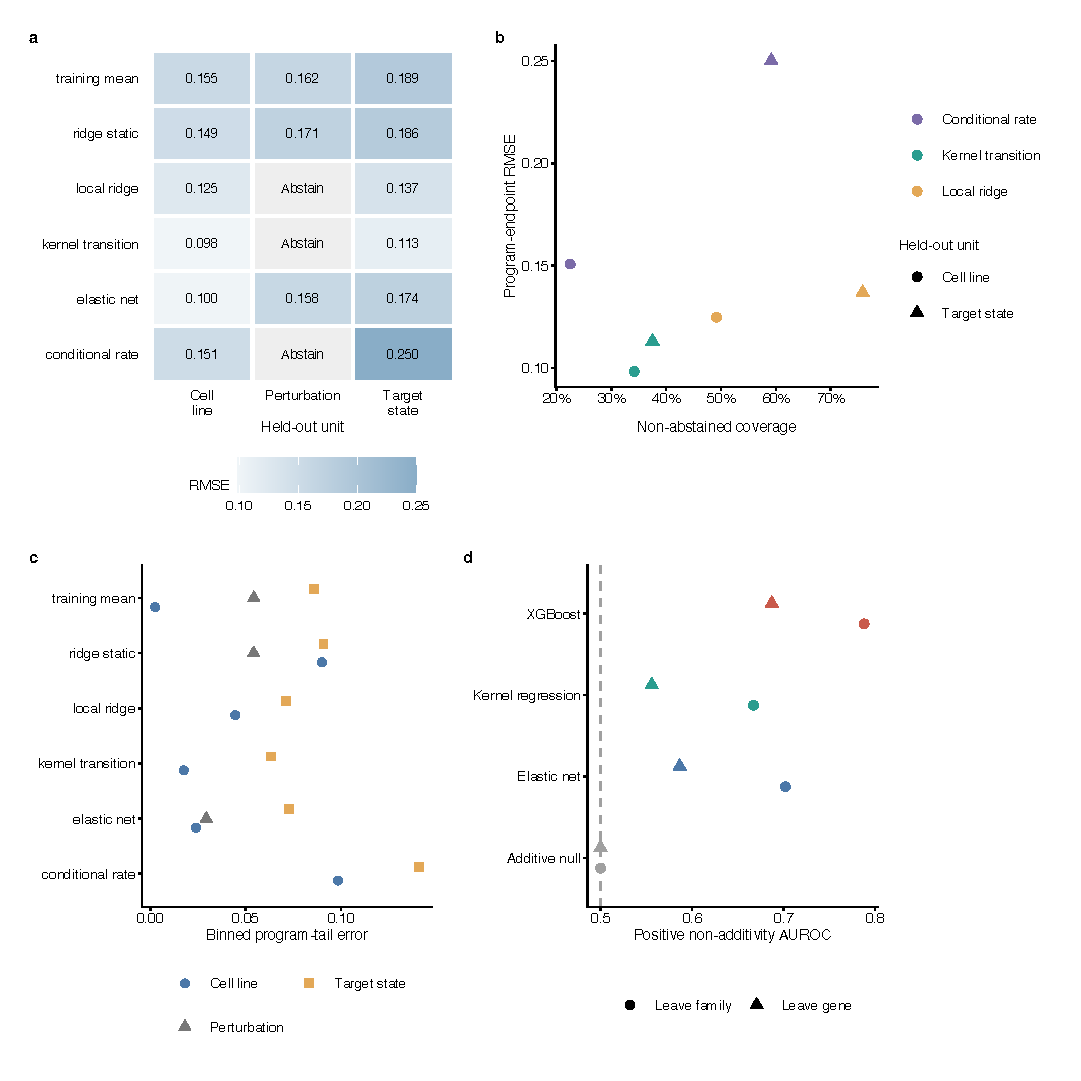
\includegraphics[width=\textwidth]{figure/Fig3_model_benchmark.pdf}
\caption{\rev{\textbf{Response-model performance depends on held-out axis and coverage.} \textbf{a}, Program-endpoint RMSE matrix for static predictors and three empirical response proxies; grey cells mark complete abstention.} \textbf{b}, Error versus non-abstained coverage; shapes encode held-out units. \rev{\textbf{c}, Binned program-tail-fraction error by split.} \rev{\textbf{d}, Positive transcriptomic non-additivity area under the receiver operating characteristic curve (AUROC) under leave-gene and leave-gene-family validation; dashed line, chance AUROC of 0.5.} Metrics are aggregated held-out estimates, not independent replicate distributions. Error values at different coverage levels do not establish model superiority. Panels a--c use the original globally fitted baseline representation.}
\label{fig:models}
\end{figure}
Performance depended on what was withheld. Under leave-cell-line validation, elastic net reached root-mean-square error (RMSE) 0.100 at full coverage. Local-response ridge reached RMSE 0.125 at 49.2\% coverage, kernel transition reached 0.098 at 34.2\%, and the conditional-rate network reached 0.151 at 22.5\%. Under leave-source-state validation, elastic net again retained full coverage with RMSE 0.097, whereas local and kernel models covered only 16.7\% and 12.5\% of cases. The conditional-rate network evaluated three of 120 cases and had RMSE 0.313. These results show that a low error on accepted predictions can coexist with a narrow applicability region.

The trade-off was clearest under leave-target-state validation. Kernel transition achieved RMSE 0.113 but covered 37.5\% of conditions; local-response ridge achieved 0.137 at 75.8\% coverage; elastic net achieved 0.174 at full coverage. The conditional-rate network covered 59.2\% but performed poorly (RMSE 0.250). Target-distance error and non-target-program divergence also depend on the accepted subset; direct model comparisons require the matched-case analysis below.

Matched-case comparisons changed the interpretation. On the 41 leave-cell-line tasks accepted by kernel transition, its RMSE was 0.0983 versus 0.1012 for elastic net; the elastic-net-minus-kernel difference was 0.00282 (95\% cell-line-cluster bootstrap interval $[-0.00130,0.00681]$). On the 45 kernel-accepted leave-target-state tasks, elastic net instead had lower RMSE (0.1050 versus 0.1131; difference $-0.00809$, interval $[-0.01464,-0.00167]$). The corresponding leave-source-state comparison used only 15 tasks (0.1278 versus 0.1280). Supplementary Fig.~S3 presents overall and program-specific selective risk--coverage curves for all four axes; numerical tables retain zero-coverage cases. These are conditional out-of-fold uncertainty estimates, not independent model-training replications.

Training-only cutoff selection did not guarantee risk transfer: at an RMSE tolerance of 0.10, local ridge accepted 19/120 cases but had outer RMSE 0.157; kernel accepted 28/120 with RMSE 0.0969, and conditional rate abstained throughout. In the separate train-fold RNA/PCA benchmark, elastic-net RMSE was 0.105 at full coverage. Kernel covered 98/120 cases with RMSE 0.0940, versus 0.0969 for elastic net on the same cases (kernel-minus-elastic difference $-0.00290$, 95\% cell-line-cluster interval $[-0.00649,0.00135]$). Coverage differed across these preprocessing and evaluation pipelines; they are not a data-matched comparison of representation architectures.

In the count-level nested scVI evaluation, elastic net gave RMSE 0.09853 at full coverage. Kernel transition accepted 96/120 tasks with RMSE 0.09407, versus matched elastic net 0.09673 (kernel-minus-elastic difference $-0.00267$, conditional 95\% line-cluster interval $[-0.00580,0.00021]$). At the exploratory inner tolerance of 0.10, kernel accepted 88/120 with RMSE 0.09035 versus matched elastic net 0.09365; the difference was $-0.00330$ [$-0.00660,-0.00037$]. \rev{The gain was small and conditional on the accepted population and exploratory threshold.} \rev{Intervals condition on fixed out-of-fold predictions and do not adjust for the multiple evaluated tolerances; they do not establish general model superiority.} The same tolerance gave outer RMSE 0.10986 for local ridge and 0.16746 for the converged rate network, so empirical training-risk targets did not uniformly transfer. The 6,000-iteration check converged all 75 rate-network fits, but its original-cutoff error remained high (76/120 accepted; RMSE 0.25532 versus matched elastic net 0.09448).

\rev{We next tested whether endpoint-error differences improved intervention choice on identical accepted drug sets within each cell line, experiment and horizon.} \rev{At the original kernel cutoff, 17 of 30 multi-drug contexts retained at least two accepted candidates.} \rev{When maximizing the apoptosis-associated tail fraction, both models chose the same drug in all 17 contexts, with 15 observed top-choice matches and mean regret 0.0042.} \rev{When minimizing the proliferation-associated fraction, kernel and elastic-net regret were 0.0248 and 0.0196, respectively (difference 0.0052; conditional 95\% cell-line-bootstrap interval $[-0.0072,0.0230]$).} \rev{The exploratory 0.10 tolerance likewise did not establish improved prioritization (Supplementary Note S2, Table S3d).} \rev{The small endpoint-RMSE gain therefore did not translate into a demonstrated decision advantage on these transcriptional objectives.}

A separate selection sensitivity evaluated 144 lower-cell-support conditions with known intervention identities using the frozen outer models. Elastic-net RMSE was 0.11990 at full coverage; kernel accepted 82/144 with RMSE 0.10330 versus matched elastic net 0.10852. Another 66 conditions had new intervention identities and were audited as unsupported. These conditional results do not separate response-estimation noise from differences in biological or experimental composition (Supplementary Note S2).

All three response-aware models abstained on every leave-perturbation case because intervention identity was absent from training. Static predictors emitted values for all cases, with RMSE 0.158--0.171, but numerical output alone does not establish mechanistic reachability. We therefore reported error jointly with non-abstained coverage and retained complete abstention as the valid result when the intervention itself was unsupported.

\subsection*{\rev{Non-additivity classes depend on transcriptional representation}}
We then quantified whether simultaneous perturbations moved cells beyond the sum of their matched single responses. Collapsing construct aliases to unique simplified conditions yielded 152 single perturbations, 131 simultaneous pairs and five controls in Norman CRISPRa. No simplified pair was counted twice. For pair $A,B$, non-additivity was estimated in a 3,591-gene response space as
\begin{equation}
I_{AB}=\Delta X_{AB}-(\Delta X_A+\Delta X_B).
\end{equation}
The target direction was defined from two matched single-perturbation response vectors, rather than from the pair outcome. Variation across eight technical GEM groups supplied within-experiment partition uncertainty.

\rev{After two-sided tests across GEM groups and Benjamini--Hochberg correction across all 131 pairs, eight pairs met the positive non-additivity rule, 71 were antagonistic, one was redundant and 51 were classified as residual (Supplementary Fig.~\ref{fig:combo}).} These labels refer to movement along a matched-single-derived transcriptional response direction. \rev{The residual class comprises pairs unresolved by the preceding classification rules and does not demonstrate changes across biological contexts.} These classes do not establish therapeutic synergy, organismal benefit, toxicity or clinical dose interaction.

The 131-pair descriptive analysis includes 14 pairs with 51--96 cells that do not enter the 269-task eligible Norman catalogue (152 singles and 117 pairs). The original labels were representation-sensitive: 113 of 131 were unchanged under log-CPM and 98 under gene-standardized log-normalized counts; seven and two of the original eight positives, respectively, remained positive. An exact technical-group sign-flip diagnostic retained seven of eight after correction. These checks assess the additive transcriptomic null within one experiment, not biological replication (Supplementary Note S3).

\begin{figure}[tbp]
\centering
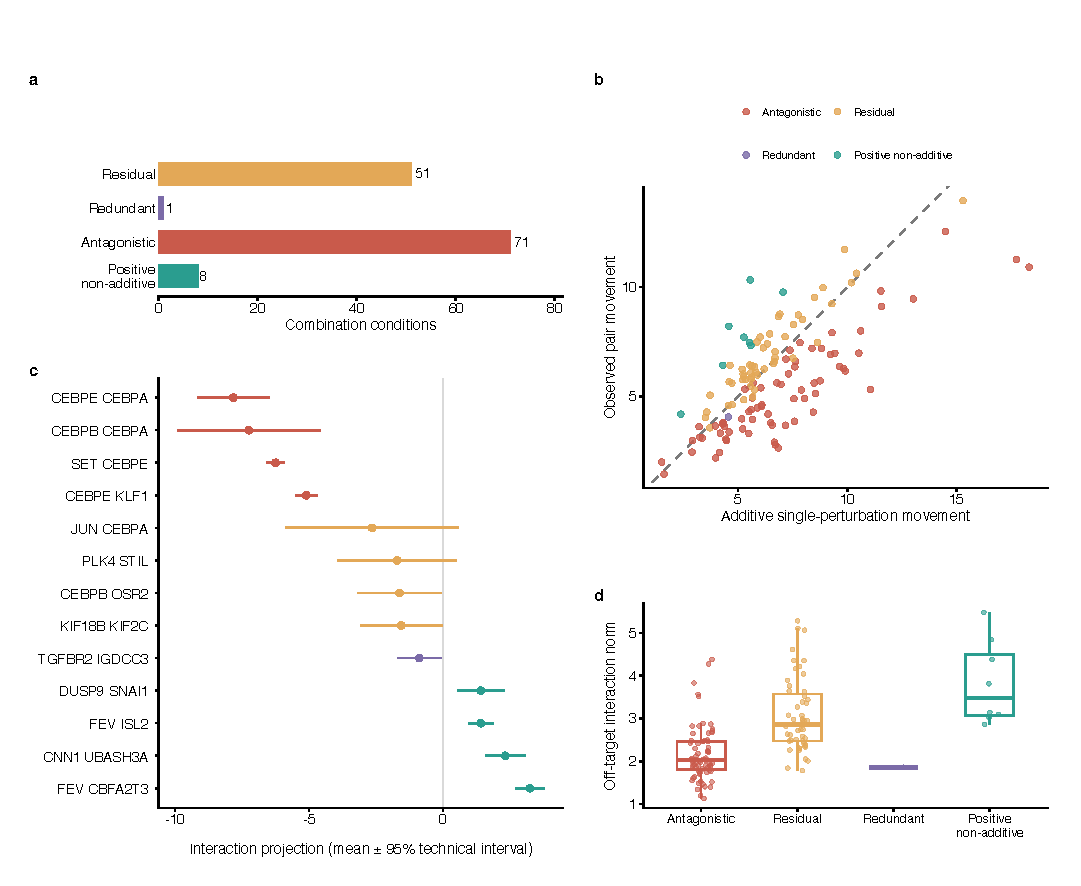
\includegraphics[width=\textwidth]{figure/Fig4_combination_control.pdf}
\caption{\textbf{Observed combinations exhibit non-additive responses.} \textbf{a}, Counts of all 131 Norman pairs by interaction class. Positive non-additive and residual replace the historical labels synergistic and context-dependent; the underlying assignments are unchanged. \textbf{b}, Observed pair movement versus the additive single-perturbation null; dashed line, equality. \textbf{c}, Mean interaction projections and 95\% $t$ intervals across eight technical GEM groups from one pooled experiment. Up to four pairs per class were selected by absolute mean projection, including the single redundant pair; this is a class-balanced illustration, not a random sample. \textbf{d}, Off-target interaction norms for all pairs, grouped by class. Boxes show median and interquartile range; whiskers extend to observations within 1.5 interquartile ranges. Points denote distinct pair conditions.}
\label{fig:combo}
\end{figure}

Strict leave-gene validation removed every pair containing a held-out gene from training and scored each pair once. \rev{Extreme gradient boosting (XGBoost) achieved interaction RMSE 1.58, Spearman $\rho=0.507$ and positive non-additivity AUROC 0.687; elastic net achieved RMSE 1.57, $\rho=0.392$ and AUROC 0.586.} Leave-gene-family validation removed all genes assigned to the held-out primary domain annotated in the Protein families (Pfam) database and evaluated 130 uniquely assigned pairs. XGBoost AUROC increased to 0.788, compared with 0.667 for kernel regression and 0.702 for elastic net. Because the response screen contains observed singles and pairs rather than a complete combinatorial intervention lattice, the one-versus-two-input endpoint was reported as constructed intervention-size classification, not as recovery of a biologically proven minimum intervention set.

Only eight of 131 pairs were positive (6.1\%). Conditional anchor-gene or primary-family cluster-bootstrap intervals for XGBoost AUROC were $[0.499,0.828]$ under leave-gene and $[0.655,0.902]$ under leave-family validation; average precision was 0.108 and 0.154, versus 0.150 and 0.160 for single-response magnitude. Some folds contain no positives. Single-response features remain measured for held-out genes, so these results describe predictions of unobserved combinations of characterized singles and do not establish general prediction of biological synergy (Supplementary Note S3).

Paired anchor-gene/family bootstrap comparisons did not establish an XGBoost improvement over summed-single-response magnitude: AUROC differences were $-0.0183$ (95\% interval $[-0.117,0.104]$) and $0.0574$ ($[-0.0546,0.167]$). Frozen-score discrimination changed under alternative normalization and technical-test labels, reinforcing its dependence on the operational interaction definition (Supplementary Note S3).

Five additional rankings used the same atomic test assignments and features constructed without observed pair outcomes (Supplementary Fig.~S1). A simple score based on the summed root-mean-square magnitude of the two matched single responses was unexpectedly competitive. It achieved leave-gene RMSE 1.48, $\rho=0.499$ and AUROC 0.705, and leave-family RMSE 1.51, $\rho=0.516$ and AUROC 0.731. Response similarity, response-network centrality, static shortest path and a Collection of Transcriptional Regulatory Interactions (CollecTRI) regulon ranking had leave-gene AUROCs of 0.375--0.438 and correlations of $-0.084$--0.087. Thus measured response magnitude can support prediction without establishing target-specific controllability. \rev{The contribution of this reanalysis is the matched comparison and sensitivity of an explicitly defined transcriptional projection class; it does not establish a new reproducible interaction taxonomy.} \rev{Independent combinatorial perturbations are required to test whether these assignments transfer beyond this pooled K562 experiment.}


\subsection*{\rev{Guide agreement does not establish target-specific RNA--ATAC responses}}

\rev{MultiPerturb provided a test of whether guide agreement distinguishes target-specific joint RNA--ATAC responses from control variation.} \rev{The processed object contained 121,651 cells, 223 guide identifiers and 99 targeted genes; 27 human ATRT targets had sufficient support for specificity testing.} \rev{Ten targets passed the original joint median cosine threshold of 0.10, but 38.9\% of two-guide and 65.5\% of three-guide non-targeting construct groups also passed it.} \rev{No target passed the non-targeting-construct test after BH correction across 27 targets (Supplementary Fig.~\ref{fig:multiome}).}

\rev{The apparent agreement also depended strongly on the control reference.} \rev{A shared reference retained median counts of 27, 26 and 25 passing targets in equal-cell resamples at 15, 30 and 50 cells per guide, while similarly sampled controls often passed.} \rev{With distinct, depth-matched control references, no target passed both modality thresholds in any tested resample.} \rev{Among 17 originally selected guides with sufficient control expression, only two pointwise target-RNA depletion intervals excluded zero.} \rev{These diagnostics identify a failure of the agreement rule to establish specificity, rather than evidence that the perturbations lack biological effects.} \rev{No modality role was assigned, and the ten agreement-selected targets did not enter the retained task catalogue (Supplementary Note S4).}

\begin{figure}[tbp]
\centering
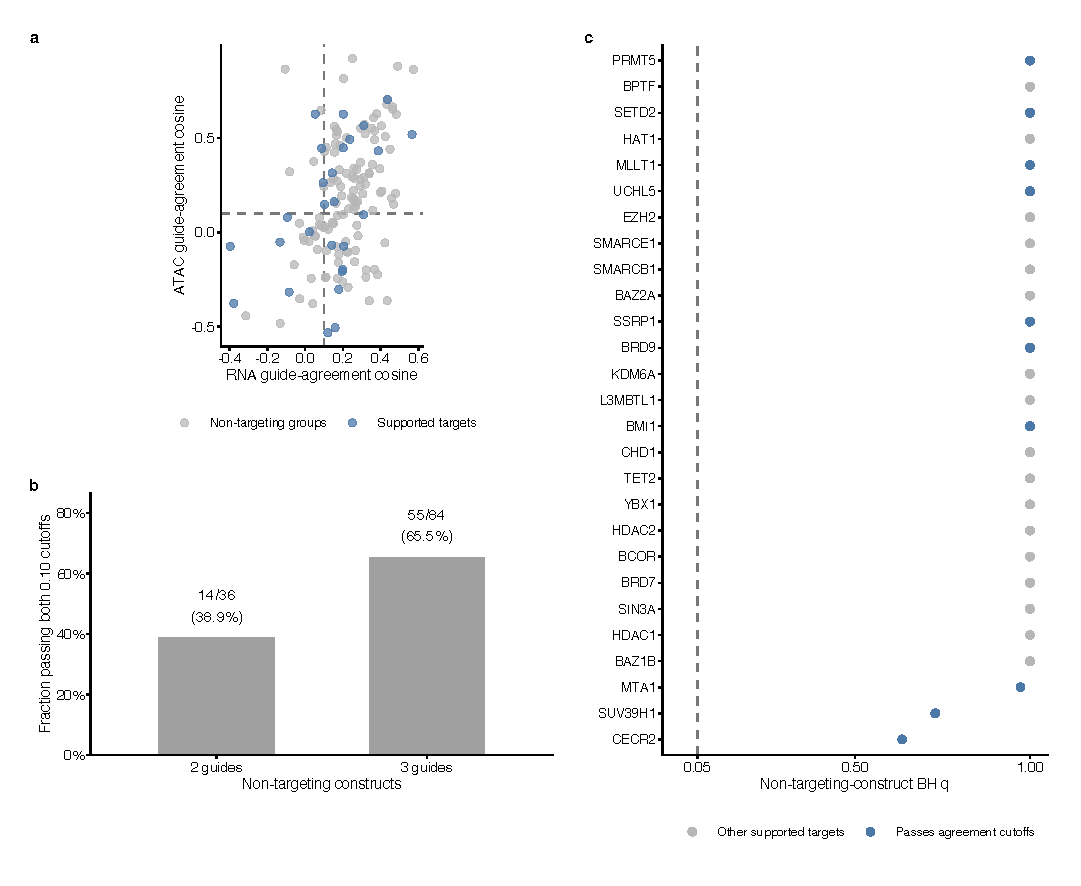
\includegraphics[width=\textwidth]{figure/Fig5_multiome_control_roles.pdf}
\caption{\rev{\textbf{Guide agreement does not establish target-specific RNA--ATAC responses.} \textbf{a}, Median leave-one-guide-out RNA and ATAC cosines for 27 supported targets and 120 overlapping non-targeting construct groups (36 two-guide and 84 three-guide); dashed lines, descriptive 0.10 cutoffs.} \rev{\textbf{b}, Non-targeting groups passing both cutoffs: 14/36 and 55/84.} \rev{These overlapping groups are not independent biological replicates.} \rev{\textbf{c}, Empirical non-targeting-construct $P$ values, BH-adjusted across 27 targets; dashed line, $q=0.05$.} \rev{Blue points identify the ten targets passing the descriptive cutoffs; none passes the specificity test (minimum $q=0.635$).}}
\label{fig:multiome}
\end{figure}

\rev{Exploratory endpoint-graph and matched-duration summaries are reported in Supplementary Notes S3 and S5 and Supplementary Figs.~S4--S5.} \rev{They describe similarity among measured endpoints and population changes during continued exposure, without identifying transition routes or continuation benefits.}

\subsection*{\rev{Assay-specific methods}}


\subsection*{Public datasets, quality control and task construction}

Only public data were used: Replogle genome-scale Perturb-seq (Figshare article 20029387),~\cite{replogle2022} Norman CRISPRa (Gene Expression Omnibus [GEO] accession GSE133344),~\cite{norman2019} MIX-Seq (Figshare \nolinkurl{10.6084/m9.figshare.10298696.v3}),~\cite{mcfarland2020} LARRY (GEO accession GSE140802)~\cite{weinreb2020} and MultiPerturb (GEO accession GSE277747).~\cite{yan2025} Dataset identities were verified against their repository accession numbers and source URLs. Large matrices were accessed sparsely or in delayed chunks. The Replogle pseudobulk Message-Digest Algorithm 5 (MD5) checksum matched the publisher value. No patient-level private data or newly generated biological samples were used.

Quality control retained provenance-preserving cell identifiers and publisher-provided or prior singlet/doublet annotations where available. Thresholds were defined by task type. Replogle tasks required at least three perturbation and three control gem groups, at least 100 cells per arm, reproducible target movement and movement larger than standardized library-size shifts. For each held-out gem group, the target program and direction were selected using the remaining groups and evaluated only in the held-out group. Eligible effects required at least 60\% selection agreement, positive held-out effects, a positive 95\% $t$ interval and Benjamini--Hochberg-adjusted $P<0.05$ across genes.

Norman conditions required at least 100 cells and positive gem-group reproducibility. MIX-Seq required at least 100 baseline and treated cells and a maximum program standard error no greater than 0.10. \rev{MultiPerturb was screened using at least 100 perturbed and control cells per target--context, at least two guides, at least 15 cells per guide, joint RNA--ATAC guide cosine above 0.10 and library-size nuisance separation.} \rev{Retention additionally required BH $q<0.05$ against the non-targeting-construct null across the 27 sufficiently supported targets; no target passed.} Complete perturbation conditions, rather than individual cells, guides or construct aliases, formed the atomic split unit.

GEM groups are treated as within-experiment partitions, not independent biological experiments. Norman groups are the eight lanes of one pooled K562 CRISPRa experiment; their intervals quantify technical partition variability conditional on that experiment. Replogle GEM-group agreement similarly does not establish independent biological replication. The two LARRY resources are different experimental arms of GSE140802, rather than independently generated validation studies. Dataset counts, task denominators, sequential exclusion counts and a source-to-analysis workflow are provided in Supplementary Tables S1--S2 and Supplementary Note S1.

Replogle endpoints were prespecified apoptosis, proliferation and stress programs. Norman condition responses were projected onto principal components and clustered by $k$-means; mean silhouette over $k=8,\ldots,24$ selected $k=18$. These clusters were treated as unlabelled response basins. \rev{MIX-Seq endpoints were nonexclusive matched-control transcriptional-program tail fractions for apoptosis, proliferation and stress.} \rev{A fraction is the estimated proportion of measured cells exceeding a program-score threshold, not a probability of a functional event.} MultiPerturb endpoints combined context-matched RNA and gene-linked ATAC movement.

Regulon and pathway layers used CollecTRI, Pathway RespOnsive GENes (PROGENy) and Hallmark axes. CollecTRI provided signed transcription-factor--target priors~\cite{collectri2023} and was kept distinct from a dataset-fitted SCENIC network.~\cite{scenic2017} PROGENy footprints, Hallmark gene sets and the decoupleR framework supplied established pathway-activity resources and scoring methodology.~\cite{schubert2018,liberzon2015,badia2022} Metabolic state was represented by an oxidative-phosphorylation expression proxy, and cell-cycle state by E2 factor (E2F) and G2/mitosis (G2/M) activities. A task-level mask recorded whether RNA, baseline-latent, pathway, cell-cycle and ATAC layers were available.

The catalogue integrates provenance and evidence labels, not numerical coordinates across studies. \rev{MIX-Seq prediction errors are compared within its three program endpoints; Norman interactions and endpoint clusters are within K562 CRISPRa; MultiPerturb specificity is within ATRT; and LARRY ranks retain resource-specific branches.} Only the shared baseline axes were used in the explicitly reported LARRY transfer analysis. A modality mask documents missing measurements but does not harmonize assays or make these endpoint scales interchangeable. Gene-level integration records context and perturbation modality; CRISPRi and CRISPRa responses are not averaged or assumed to have the same direction.

\subsection*{Empirical response models and abstention}

\rev{MIX-Seq models predicted three transcriptional-program tail fractions.} Elastic net used \texttt{glmnet} with $\alpha=0.5$. Local-response ridge fitted distance-weighted ridge models within 45 neighbours. Kernel transition used a Gaussian kernel over as many as 60 neighbours and prioritized the same intervention. The conditional-rate network used a single-hidden-layer network to estimate a constant endpoint-derived logit rate from a 0.1 prior; three random initializations formed an ensemble.

Response-aware models abstained when intervention identity was absent from training, when the source state exceeded the 95th percentile of training nearest-neighbour distance, when kernel support was below ten, or when uncertainty was non-finite or exceeded 0.15. Leave-source-state used five clusters of baseline latent profiles and was distinct from leave-cell-line. Performance was computed only for accepted predictions, and coverage was reported for every split--model pair.

Of the 151 eligible MIX-Seq tasks, the prediction table contains 120 chemical tasks; the other 31 are GPX4 genetic tasks without matched chemical-baseline model rows. The 100-cell gate retains these 120 of 1,044 chemical model rows; all 120 already pass the probability-standard-error gate. Program endpoints, baseline embeddings and source-state clusters were constructed before cross-validation; leave-target-state groups use the observed dominant endpoint program. Model scaling and fitting use training rows, but the original benchmark is conditional on this frozen task catalogue and representation. \rev{Outcome-defined target groups test retrospective reconstruction across measured response classes and cannot serve as prospectively assignable target labels.} Replogle response-dependent eligibility and Norman basin learning likewise precede this catalogue; neither supplies MIX-Seq prediction labels. \rev{Query profiles are DMSO controls measured at the matched treatment horizon, including for held-out cell lines.} \rev{Thus the cell-line benchmark evaluates generalization to experimentally characterized control conditions, rather than intervention prediction using pretreatment information alone.} \rev{The archived QC mask, gene availability, program definitions and 120-task panel remain fixed even in the nested scVI evaluation.} \rev{A prospective test would fix eligibility, pretreatment inputs and the target definition before observing treatment outcomes.}

Unseen-intervention rejection is a design restriction: these response models require an intervention represented in training. It is distinct from distance-, support- and uncertainty-based rejection within known interventions and does not demonstrate learned detection of biological impossibility. \rev{The uncertainty cutoff 0.15 is a heuristic tolerance on the program-tail-fraction scale, not a calibrated confidence level.} Supplementary Note S2 reports comparisons on identical accepted tasks, error--coverage curves, cutoff sensitivity and resampling uncertainty, including separate program endpoints. These checks quantify the risk of using unsupported endpoint estimates to select interventions without treating abstention as proof of control.

The baseline encoder uses single-cell variational inference (scVI).\cite{lopez2018scvi} We additionally nested variable-gene selection, scVI fitting, predictor scaling, elastic-net penalties and response-model cutoff selection within five outer and four inner cell-line folds. The 25 training executions cover 15 distinct reference-cell subsets because symmetric inner folds share training cells. Every held-out line's baseline cells were excluded before feature selection and training; query encoding used frozen parameters. Supplementary Note S2 specifies the fixed auxiliary reference panel, low-cell-support queries and endpoint-rate-network optimization check.

Earlier conditional checks selected uncertainty cutoffs using four grouped inner cell-line folds within each of the five outer cell-line folds, under exploratory RMSE tolerances of 0.10, 0.15 and 0.20. At least ten accepted inner cases from three lines were required. A separate RNA-based benchmark selected variable genes, fitted PCA and scaled features using outer-training baseline contexts only, then projected held-out cell lines (Supplementary Note S2).

\rev{For retrospective intervention prioritization, candidate drugs shared a cell line, experiment and horizon, with at least two kernel-accepted interventions.} \rev{Both models ranked exactly the same candidate set, separately maximizing the apoptosis-associated tail fraction and minimizing the proliferation-associated fraction.} \rev{Regret was the observed gap between the best accepted intervention and the intervention selected from predictions; contexts received equal weight.} \rev{Ties were resolved by intervention identity without using treatment outcomes.} \rev{Intervals used 10,000 cell-line-cluster bootstrap draws conditional on fixed predictions, candidate sets and policies (Supplementary Note S2).}

\subsection*{Lineage-supported local response geometry}

Day-2 LARRY cells were aggregated by clone. Within each future condition, baseline features were standardized and projected by principal components. Neighbourhood size was
\begin{equation}
k=\min\left(60,\max\left(15,\left\lfloor\sqrt{n}\right\rfloor\right),n-1\right).
\end{equation}
For each state-feature association, neighbourhoods were recomputed after excluding the tested feature's constituent axes. For example, hypoxia, reactive oxygen species and unfolded protein response scores were excluded when testing stress. If $\lambda_i$ are the non-negative eigenvalues of local descendant-probability covariance and $p_i=\lambda_i/\sum_j\lambda_j$, effective rank was
\begin{equation}
r_{\mathrm{eff}}=\exp\left\{-\sum_i p_i\log p_i\right\}.
\end{equation}
Branches with mean local probability below 0.05 were called locally unsupported. Regularized reciprocal diagonal variance, using $10^{-4}$ regularization, defined a local inverse-variance score that summarized the concentration of lineage-supported descendant variation. This score was used only as a local-geometry diagnostic and was distinct from the intervention-based relative-effort proxy used in the response-path analysis.

Linear models included stress, oxidative metabolism, mitochondrial fraction, chromatin-regulator activity, cell cycle and future condition where applicable. The focal feature was residualized on the remaining state features at the unique-clone level. Its residual was permuted across clones 999 times and recombined with its fitted component. Two-sided empirical $P$ values were adjusted across the five tested state features within dataset and outcome. Cluster-robust asymptotic estimates were retained as diagnostics rather than primary inference.

Additional high-versus-low stress comparisons used descriptive overlap weights,\cite{li2018overlap} with quality/abundance-only and quality-plus-state specifications. Each clone initially had total weight one; 499 clone bootstrap draws re-estimated the balancing weights while keeping the original geometry fixed. We also compared shared clones across future cytokine conditions, with descendant-support restrictions and paired label-swap diagnostics (Supplementary Note S1).

\rev{A controlled simulation generated stress-independent intrinsic branch probabilities using condition-specific composition offsets and clone-level logistic-normal variation.} \rev{The same intrinsic probabilities were observed at recorded, equalized or permuted descendant depths, with fixed or randomized condition-matched neighbourhoods.} \rev{We also repeated the analysis in the recorded ten-descendant subset with rebuilt geometry.} \rev{Two hundred latent draws per resource and dispersion setting were reused across nine observation scenarios; three dispersion settings were evaluated (Supplementary Note S6).}

Cross-dataset transfer was evaluated between the two LARRY resources using the baseline axes shared by both datasets. Models fitted in one resource were applied to the other in both transfer directions. Transfer performance was summarized by Spearman correlations for differentiation propensity, transition entropy and rare-fate probability.

\subsection*{Combination effects, grouped validation and multiome reproducibility}

Norman counts were transformed as $\log(1+10^4 x_{gc}/L_c)$, where $L_c$ is the total count for cell $c$, then averaged by unique simplified condition and GEM group. This is log-normalized counts per ten thousand, not log-CPM. The additive null for each pair was the sum of its two matched single responses. Interaction classes use the projection and its GEM-group interval; exact rules, all 131 effect sizes and adjusted $P$ values, technical-group bootstrap checks and normalization sensitivity are reported in Supplementary Note S3. Two-sided $t$ tests across the eight technical groups were adjusted across 131 pairs. These intervals do not quantify between-experiment biological variation.

Leave-gene validation removed every pair containing a held-out gene from training and assigned each test pair to one fold. Leave-family validation used \texttt{org.Hs.eg.db} Pfam annotations, selected one primary domain per assayed gene deterministically and removed genes assigned to the held-out primary domain. Each annotated test pair was scored once. Predictor specifications explicitly prohibited features derived from the observed pair response.

Measured single-gene responses remain available for test genes. Thus leave-gene and leave-family prediction concern unseen combinations of experimentally characterized singles, not wholly uncharacterized genes. The small positive class is evaluated descriptively with prevalence, precision--recall performance and uncertainty intervals (Supplementary Note S3).

\rev{MultiPerturb RNA and gene-linked ATAC counts were library-normalized and contrasted with context-matched non-targeting controls.} \rev{Median leave-one-guide-out cosine measured agreement among guides targeting the same gene.} \rev{Specificity was evaluated against all sufficiently populated non-targeting construct groups, with BH correction across 27 supported targets.} \rev{Equal-cell analyses contrasted a shared control anchor with distinct, cell-count- and library-matched references for each guide.} \rev{The original movement-quartile role labels were not retained because these controls did not validate their target specificity.}

\subsection*{Extended baselines, evidence synthesis and sequence analysis}

Extended Norman baselines reused the exact leave-gene and leave-primary-Pfam assignments. Differential-response magnitude summed the root-mean-square matched single responses. Response similarity was the cosine between the two single responses. A response graph connected absolute single-response cosines above their 90th percentile; node strength defined network centrality, and inverse cosine weight defined static shortest-path distance. The signed CollecTRI score projected single responses onto regulons with at least five measured targets and combined regulator-space magnitude with pair similarity. Within each split, univariate calibration and intervention-size thresholds were fitted using training-pair outcomes only.

Architecture names were reserved for original implementations.~\cite{scenic2017,gears2024,scgen2019,cpa2023,chemcpa2022,txpert2026} An applicability audit found that the available chemCPA checkpoint and scGen scripts used incompatible Library of Integrated Network-based Cellular Signatures (LINCS) schemas, while no compatible fitted SCENIC object, GEARS checkpoint/runtime or TxPert implementation was available.

\rev{The perturbation-supported class required eligible transcriptional movement in at least one biological context and excluded MultiPerturb targets failing the specificity test.} \rev{Control-node assessment required measured support in at least two independent biological contexts, consistency with observed combination behaviour and target-path specificity.} \rev{A candidate could be assessed only when all required assay types were available; missing measurements were not negative tests.} Measurements from repeated K562 resources were counted as evidence from one biological context rather than as independent contextual replication. A validated control node would further require held-out cross-cell-line reachability and favourable non-target-program behaviour relative to competing interventions.

\rev{For the exploratory endpoint-graph analysis, relative effort was intervention size divided by squared endpoint-response magnitude.} Lower values therefore indicated greater observed response movement per intervention component. This quantity was used only as an empirical ranking measure and was not interpreted as physical control energy.

For an orthogonal functional check, exact CRISPRa guide identities were matched to the original authors' two bulk-growth phenotype maps, with the published label mappings. Normalized growth scores were compared descriptively across fixed RNA basins; unmatched or non-finite guide measurements were not imputed. This is a separate assay in the same source study, not a new biological context (Supplementary Note S3).\cite{norman2019}

\rev{Exploratory Norman endpoint-graph components were computed within response clusters using cosine thresholds 0.70, 0.80 and 0.90; 0.80 was the original descriptive threshold.} Same-drug MIX-Seq duration contrasts were evaluated only when both 6-h and 24-h population endpoints existed in the same cell line. Drug switches, Norman pair order and commitment locks were assigned \texttt{abstain} because no observed transition supported them.

\subsection*{Metrics and software}

\rev{Metrics comprised endpoint RMSE, target-distance error, non-target-program divergence, threshold accuracy, high-program-tail-fraction recall, binned fraction error, interaction RMSE, Spearman correlation, positive non-additivity AUROC and coverage.} State-association and technical interaction tests were two-sided; guide-agreement and paired-context label-swap diagnostics used upper-tail randomization or empirical-null comparisons. Statistical analyses and figures used R; nested scVI training used Python, scvi-tools 1.4.3 and PyTorch 2.5.1 on CPU. Executed versions and seeds are supplied with the code.


\clearpage
\section*{\rev{Supplementary Note S8. Harmonized features and study-held-out evaluation}}

\rev{The common-gene intersection used measurement annotations from Replogle K562, Norman, MIX-Seq, Adamson and Frangieh before external response evaluation.} \rev{Duplicated count features were summed before log transformation.} \rev{Every source used the same 7,848-gene library denominator; no feature outside the measured intersection entered scoring.} \rev{Complete module membership, original and retained coverage, source normalization totals and cell identities are supplied in the Supplementary Data and reproducibility archive.} \rev{The scores summarize RNA expression.} \rev{Hallmark sets overlap, and score correlations do not establish independent pathway activation or causal mechanisms.}

\subsection*{\rev{Supplementary Table S6. Retained score membership.}}

\begin{tabular}{p{0.48\textwidth}rr}
\toprule
\rev{Expression summary} & \rev{Positive members} & \rev{Negative members}\\
\midrule
\rev{Apoptosis-associated short module} & \rev{10} & \rev{4}\\
\rev{Proliferation-associated short module} & \rev{12} & \rev{3}\\
\rev{Stress-associated short module} & \rev{11} & \rev{0}\\
\rev{UPR} & \rev{91} & \rev{0}\\
\rev{E2F} & \rev{187} & \rev{0}\\
\rev{G2/M} & \rev{176} & \rev{0}\\
\rev{p53} & \rev{116} & \rev{0}\\
\rev{TNF/NF-$\kappa$B} & \rev{82} & \rev{0}\\
\rev{Interferon-$\gamma$} & \rev{79} & \rev{0}\\
\rev{mTORC1} & \rev{175} & \rev{0}\\
\rev{Oxidative phosphorylation} & \rev{178} & \rev{0}\\
\rev{Hypoxia} & \rev{86} & \rev{0}\\
\bottomrule
\end{tabular}

\rev{Complete-condition support, rather than an observed response cutoff, defined the cross-study panel.} \rev{Replogle contributed 358 genes in 48 technical GEMs; Norman contributed 280 conditions in eight technical GEMs; chemical MIX-Seq contributed thirteen drugs in 169 experiment--line--horizon contexts from 109 lines.} \rev{These produced 2,151, 2,180 and 527 eligible units, respectively.} \rev{Each intervention and context can contribute several rows; neither rows nor expression axes are independent biological replicates.}

\begin{figure}[H]
\centering
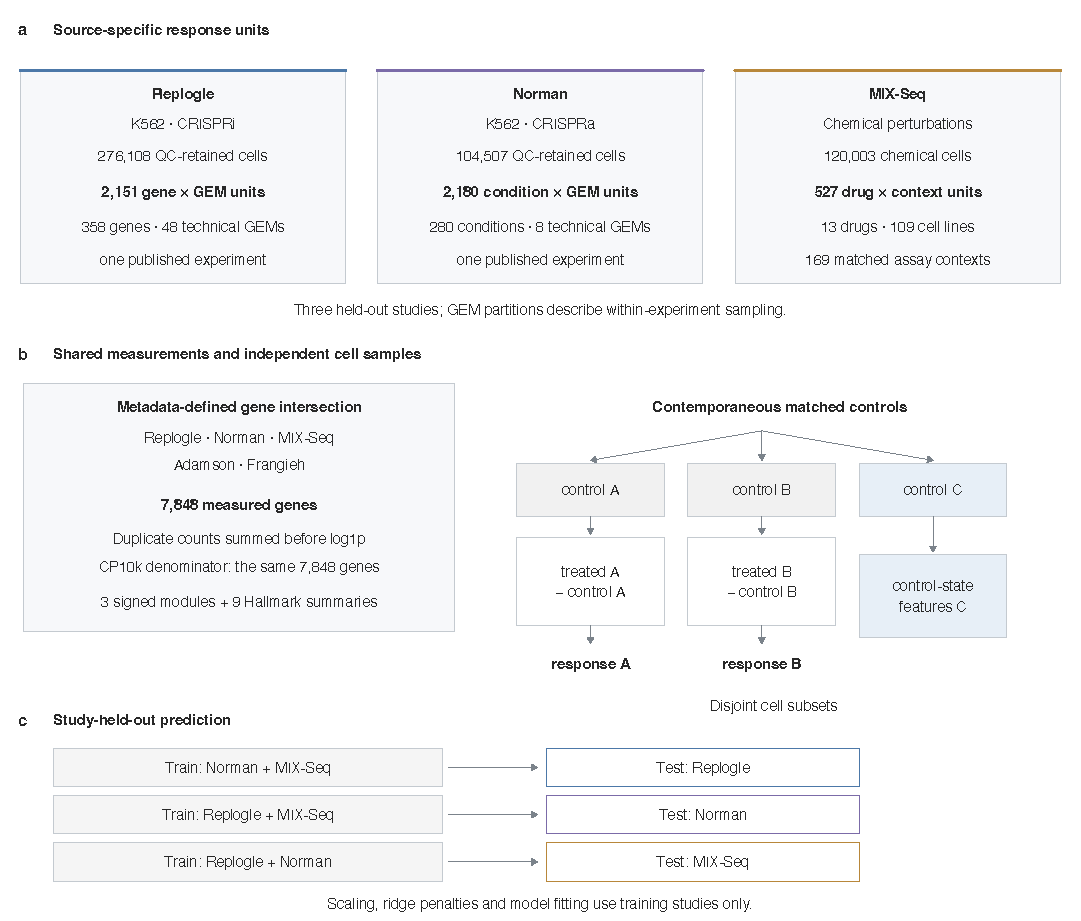
\includegraphics[width=\textwidth]{figure/Fig_cross_study_design.pdf}
\caption{\rev{\textbf{Observation design for study-held-out response evaluation.} The harmonized five-source measurement space contains 7,848 gene symbols and twelve fixed scores.} \rev{Three primary sources supply the response-model benchmark.} \rev{Control subset C provides context-state features, control A/B subsets anchor independently partitioned treated A/B responses, and the evaluation study is excluded from scaling, model fitting and tuning.} \rev{A measured pilot-response input is distinguished from a context-only model.} \rev{Technical partitions and random cell subsets do not provide independent biological replication.} \rev{External-study candidate evaluation uses frozen discovery choices.}}
\label{fig:supp-common-design}
\end{figure}

\rev{The fitted response comparator included the twelve signed pilot-A responses, log total treated count, log A-plus-B control count and the control-C mean log common-library size; the added-state model additionally included the twelve control-C means and twelve log variances, with $10^{-4}$ variance regularization.} \rev{The state-only specifications excluded pilot-response values.} \rev{Ridge penalties were selected by inner leave-study-out error, with equal weights assigned to the two training studies.} \rev{All ten fixed cell partitions are retained.} \rev{The target-mutation test changed every held-out B response and found exactly unchanged predictions and selected penalties.} \rev{Cell identifiers confirmed disjoint A, B and C control pools and disjoint treated A/B pools.}

\rev{The primary target was the raw-score response B.} \rev{Joint errors give every eligible unit and every included axis equal evaluation weight; core-module, Hallmark and all-twelve summaries are reported separately because score variances differ.} \rev{Sampling precision used log squared A--B response disagreement.} \rev{The analytic comparator was constructed from within-arm score variances and sample sizes.} \rev{It outperformed learned reliability predictors on primary log-RMSE in all three held-out studies.} \rev{Across ten partitions, adding state to the sampling/pilot specification worsened reliability error in eight MIX-Seq, six Norman and eight Replogle partitions.} \rev{These computational resamples do not show that state never contains predictive information.}

\rev{For response prediction, pilot-plus-state minus pilot-only core-module RMSE was 0.027709 in MIX-Seq, 0.006637 in Norman and 0.000676 in Replogle.} \rev{Crossed intervention/context intervals were $[0.0181,0.0398]$, $[0.00529,0.00798]$ and $[-0.000635,0.00206]$.} \rev{Norman anchor-gene clustering gave $[0.005177,0.008081]$.} \rev{All twelve-axis point estimates favoured pilot-only ridge, but the unshrunk pilot was the stronger MIX-Seq comparator.} \rev{The intervals condition on the original predictions and cell partitions; they do not refit models or quantify new-study sampling uncertainty.}

\rev{Three prespecified cross-program associations per study used independent response halves, adjustment for context and sampling support, and joint correction across nine tests.} \rev{Stress--apoptosis coupling changed sign between MIX-Seq and Norman.} \rev{Apoptosis--proliferation coupling was negative in all three sources, but Norman anchor-gene sensitivity did not survive correction.} \rev{These associations do not establish a new conserved mechanism.} \rev{The complete coefficient, resampling and multiplicity tables remain available, including analyses with exchanged response halves and all fixed cell partitions.}

\section*{\rev{Supplementary Note S9. Independent-study priority and axis validation}}

\rev{The discovery-only three-module priority selected a dominant program and sign in Replogle and retained the same choices for external evaluation.} \rev{Source support required at least 100 retained cells and three GEM groups without effect-significance filtering.} \rev{The Adamson panel required at least 100 external cells per gene, and the primary Frangieh panel required at least thirty cells under the unstimulated condition.} \rev{These rules retained thirty and nineteen genes, respectively, with seventeen in co-culture.} \rev{Adamson's 10X010 experiment was enriched for UPR-related perturbations; it provides a separately generated K562 study, not an unbiased genome-wide validation population.} \rev{The three melanoma conditions come from one patient-derived model in a separate CRISPR-knockout study.}

\begin{figure}[H]
\centering
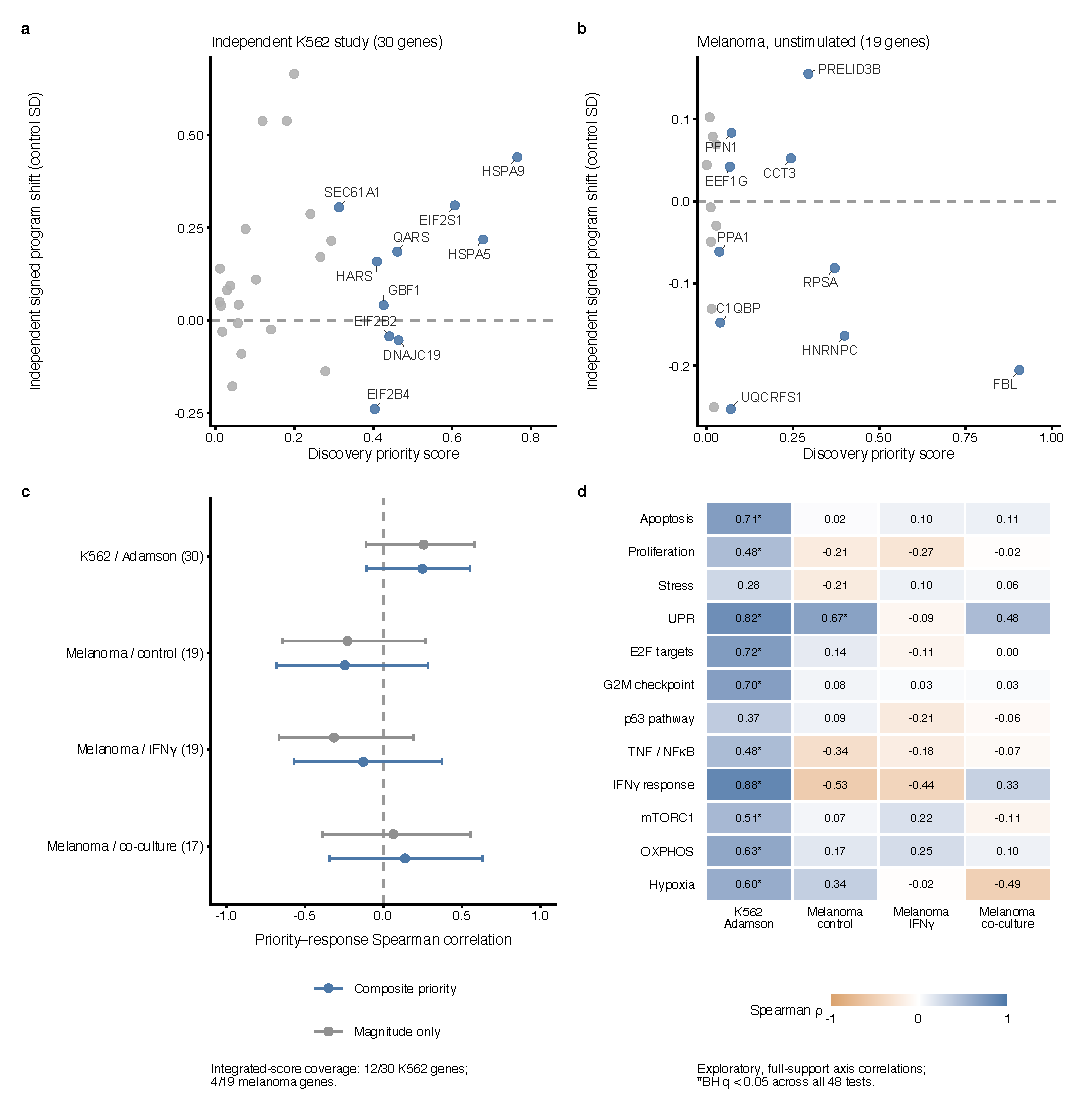
\includegraphics[width=\textwidth]{figure/Fig_independent_candidate_validation.pdf}
\caption{\rev{\textbf{The initial aggregate candidate priority does not validate externally.} Discovery scores and program directions were frozen before external effect evaluation.} \rev{Gene-level response scatterplots and ranking estimates retain all eligible genes; top-ten comparisons use the same program and sign chosen in discovery.} \rev{Simple response magnitude and model-derived priorities are evaluated on identical covered panels.} \rev{The complete twelve-axis/four-condition family is included rather than selecting only positive associations.} \rev{Intervals are conditional gene-bootstrap intervals, and technical or cell resamples are not independent biological experiments.}}
\label{fig:supp-initial-priority}
\end{figure}

\rev{The initial score correlated weakly with external directional effect in Adamson ($\rho=0.249$; $95\%$ interval $[-0.106,0.552]$) and negatively in unstimulated melanoma ($\rho=-0.246$; $[-0.679,0.285]$).} \rev{Top-ten-minus-remainder mean differences were $-0.0052$ ($[-0.165,0.145]$) and $-0.0386$ ($[-0.146,0.076]$), respectively.} \rev{Seven of ten Adamson and four of ten melanoma priorities had the selected response sign.} \rev{Equal-cell analyses did not restore a consistent advantage.} \rev{The discovery top-ten Adamson set was identical under simple dominant-magnitude ranking.} \rev{A secondary priority derived from the study-held-out model covered only twelve Adamson and four melanoma genes; missing predictions were not extrapolated.} \rev{On that restricted Adamson panel it did not establish an improvement over the matched pilot-only priority.}

\rev{The all-axis follow-up used two-sided permutation tests and BH correction across twelve axes in Adamson and three melanoma contexts, giving one family of 48.} \rev{UPR was the only axis significant in both Adamson and unstimulated melanoma.} \rev{This selection was exploratory.} \rev{The original UPR correlations were 0.8234 ($95\%$ interval $[0.6393,0.9159]$) and 0.6737 ($[0.2750,0.9043]$); corresponding $q$ values were 0.000960 and 0.00840.} \rev{Interferon-$\gamma$ and co-culture correlations were $-0.0895$ and 0.4828 and did not survive correction.} \rev{A significant association in one context and a nonsignificant association in another is not evidence of a context difference.} \rev{Direct paired context tests over shared genes did not survive correction across 24 contrasts; the control-minus-interferon UPR contrast had unadjusted $P=0.0288$ but adjusted $q=0.317$.}

\rev{Removal of the perturbed UPR gene from the score numerator alone gave Adamson and unstimulated-melanoma correlations 0.8229 and 0.7035, with sensitivity $q$ values 0.000960 and 0.00720 when replacing those four UPR tests in the complete family.} \rev{The exact all-target normalization control additionally subtracted each targeted gene's raw counts from the normalization library whenever measured, including non-UPR targets.} \rev{Matched-control moments and every logarithmic term were recomputed.} \rev{Its correlations remained 0.8229 ($95\%$ interval $[0.6158,0.9289]$; sensitivity $q=0.000960$) and 0.6825 ($[0.2567,0.8897]$; $q=0.0126$); all corrected effects and tests are supplied without altering the initial rankings.}

\rev{Minimal one-covariate-at-a-time rank checks considered source and external cell counts, target expression, proliferation/E2F, generic response magnitude and essentiality.} \rev{Leave-one-gene-out UPR correlations ranged from 0.804 to 0.858 in Adamson and 0.616 to 0.783 in unstimulated melanoma.} \rev{These are influence checks, not multivariable causal adjustment.} \rev{Equal-thirty-cell resampling in both studies gave median correlations of 0.636 in Adamson and 0.314 in melanoma; the melanoma simulation range included zero.} \rev{A fourteen-gene single-guide melanoma analysis had median correlation 0.132.} \rev{The small external melanoma panel is therefore sensitive to response-estimation precision.}

\rev{Conserved rank did not provide calibrated effects.} \rev{Only nine of nineteen melanoma UPR response signs agreed with K562.} \rev{Copying the twelve-axis discovery vector gave RMSE 0.380 in Adamson and 0.353 in unstimulated melanoma, compared with 0.356 and 0.149 for zero response and 0.325 and 0.237 for the generic discovery mean.} \rev{Relative ordering, effect direction and effect amplitude must therefore remain separate claims.}

\section*{\rev{Supplementary Note S10. Source-frozen UPR follow-up in a held-out cell context}}

\rev{The RPE1 follow-up was motivated by the exploratory external UPR correlations.} \rev{Its endpoint, eligibility, source score, nested top-ten/top-twenty lists, simple comparators, matching rules, random modules and inference code were fixed before reading RPE1 expression for this analysis.} \rev{This is an outcome-blind computational holdout within the Replogle study, not a prospectively conducted perturbation experiment or an independent source study.}

\rev{The shared measurement universe contained 6,780 genes and ninety UPR members, with NFYA absent from the RPE1 matrix and removed from both contexts.} \rev{Source counts for duplicate symbols were aggregated before transformation.} \rev{The primary source score removed the targeted UPR member from the numerator, recalculated control moments and used the fixed common-library denominator.} \rev{Exact all-target denominator exclusion was retained as a sensitivity.} \rev{The five-source analyses use the 7,848-gene universe; the targeted RPE1 evaluation uses the separately defined 6,780-gene universe.}

\rev{Source support required at least 100 retained cells and at least three technical GEMs with five target cells each.} \rev{RPE1 support required at least 100 published cells and three GEM labels.} \rev{The intersecting panel contained 438 genes; stricter RPE1 within-GEM support retained 390.} \rev{Of the 438, 65 targeted genes lacked a measured source expression feature and seventeen lacked a usable DepMap essentiality value, with fourteen overlapping; no unmeasured value was replaced by zero.} \rev{All actual UPR top-twenty genes had the four matching covariates.} \rev{The primary matched comparison therefore retained the complete twenty selected genes and one hundred distinct background genes.} \rev{Standardized generic-magnitude differences after matching were 0.231 for the top twenty and 0.321 for the top ten, so residual imbalance remains relevant to interpretation.}

\rev{One hundred random ninety-gene modules were matched to UPR source-control expression and detection bins.} \rev{All 9,000 draws matched the exact bins; no expansion was needed.} \rev{They comprised 4,402 distinct genes, with within-module sampling without replacement and UPR members excluded.} \rev{Every random module and source-frozen ranking was retained, including failed utility matches.} \rev{Eighty-four of one hundred primary random-module top-twenty lists lacked complete matching covariates, limiting matched-null specificity inference on that full panel.} \rev{Before outcome access, a separate sensitivity uniformly restricted UPR, all random modules and all comparator rankings to the same 370 complete-covariate candidate genes.} \rev{All 101 matching lists were estimable in that population, and the actual UPR top-twenty membership was unchanged.} \rev{This sensitivity was not substituted for the primary 438-gene Holm-adjusted family.}

\rev{The signed 438-gene source--RPE1 correlation was 0.3775, with conditional gene-bootstrap interval $[0.2895,0.4614]$ and Holm-adjusted $P=0.000300$.} \rev{The primary top-twenty matched gap was 0.3288 ($95\%$ interval $[0.0903,0.5849]$), and the nested top-ten gap was 0.5731 ($[0.2167,0.9651]$); both adjusted $P$ values were 0.000400.} \rev{Crossed gene/matched-set and shared-GEM wild intervals remained positive.} \rev{The stricter 390-gene population had correlation 0.4031 ($[0.3071,0.4956]$).} \rev{These are conditional associations and relative signed-response comparisons.}

\subsection*{\rev{Supplementary Table S7. Fixed UPR top-twenty list and observed effects.}}

\begin{tabular}{rlrrrrr}
\toprule
\rev{Rank} & \rev{Gene} & \rev{K562 $d$} & \rev{RPE1 $d$} & \rev{Source $f$} & \rev{K562 cells} & \rev{RPE1 cells}\\
\midrule
\rev{1} & \rev{POLRMT} & \rev{0.639} & \rev{0.079} & \rev{0.933} & \rev{176} & \rev{212}\\
\rev{2} & \rev{GBF1} & \rev{0.760} & \rev{0.934} & \rev{0.778} & \rev{141} & \rev{100}\\
\rev{3} & \rev{GMPPB} & \rev{0.528} & \rev{0.144} & \rev{0.833} & \rev{145} & \rev{101}\\
\rev{4} & \rev{RPS13} & \rev{0.533} & \rev{-1.145} & \rev{0.625} & \rev{123} & \rev{132}\\
\rev{5} & \rev{PNPT1} & \rev{0.498} & \rev{0.015} & \rev{0.667} & \rev{108} & \rev{150}\\
\rev{6} & \rev{UPF2} & \rev{0.378} & \rev{0.998} & \rev{0.714} & \rev{122} & \rev{113}\\
\rev{7} & \rev{SPCS3} & \rev{0.413} & \rev{0.795} & \rev{0.636} & \rev{159} & \rev{145}\\
\rev{8} & \rev{DNAJC19} & \rev{0.283} & \rev{0.050} & \rev{0.841} & \rev{360} & \rev{127}\\
\rev{9} & \rev{MANF} & \rev{0.382} & \rev{0.112} & \rev{0.600} & \rev{129} & \rev{178}\\
\rev{10} & \rev{UFL1} & \rev{0.301} & \rev{0.448} & \rev{0.750} & \rev{143} & \rev{115}\\
\rev{11} & \rev{RBM10} & \rev{0.209} & \rev{0.078} & \rev{1.000} & \rev{116} & \rev{136}\\
\rev{12} & \rev{ALG14} & \rev{0.282} & \rev{0.555} & \rev{0.733} & \rev{168} & \rev{115}\\
\rev{13} & \rev{RPL7} & \rev{0.253} & \rev{-1.335} & \rev{0.767} & \rev{266} & \rev{122}\\
\rev{14} & \rev{HSP90B1} & \rev{0.190} & \rev{0.112} & \rev{1.000} & \rev{102} & \rev{144}\\
\rev{15} & \rev{TIMM13} & \rev{0.239} & \rev{-0.149} & \rev{0.765} & \rev{162} & \rev{123}\\
\rev{16} & \rev{NELFCD} & \rev{0.223} & \rev{-0.659} & \rev{0.812} & \rev{180} & \rev{113}\\
\rev{17} & \rev{GARS} & \rev{0.214} & \rev{0.093} & \rev{0.783} & \rev{235} & \rev{120}\\
\rev{18} & \rev{SMARCB1} & \rev{0.213} & \rev{-0.149} & \rev{0.769} & \rev{170} & \rev{141}\\
\rev{19} & \rev{MFN2} & \rev{0.195} & \rev{0.085} & \rev{0.833} & \rev{121} & \rev{224}\\
\rev{20} & \rev{LETM1} & \rev{0.234} & \rev{-0.178} & \rev{0.667} & \rev{119} & \rev{163}\\
\bottomrule
\end{tabular}

\rev{Ranks one to ten form the fixed top-ten subset.} \rev{Effects are signed matched-GEM contrasts in applicable control standard deviations; $f$ is the positive-contrast fraction among supported source GEMs.} \rev{The ranking was fixed before RPE1 expression evaluation.} \rev{Cells and technical partitions are not independent cultures.}

\rev{The top-twenty mean signed RPE1 effect was 0.0442 ($95\%$ matched-set interval $[-0.2111,0.2792]$), compared with $-0.2845$ ($[-0.4036,-0.1744]$) in its background.} \rev{Fourteen selected genes had positive effects.} \rev{The top-ten mean was 0.2430 ($[-0.1543,0.5850]$), with nine positive genes, compared with background $-0.3301$.} \rev{Absolute-effect gaps were 0.0857 ($[-0.0415,0.2143]$) and 0.0893 ($[-0.1264,0.2759]$).} \rev{The validated comparison is therefore relative signed UPR expression, not uniformly positive activation or stronger absolute responses.} \rev{Leaving out any one matched set retained positive gaps: 0.2589--0.3787 for the top twenty and 0.4528--0.6651 for the top ten.} \rev{Leaving out one gene changed the overall signed correlation only from 0.3732 to 0.3865.}

\rev{Exact own-target numerator-and-denominator exclusion in both contexts retained correlation 0.3784 ($95\%$ interval $[0.2807,0.4599]$), top-twenty gap 0.3279 ($[0.0767,0.5878]$) and top-ten gap 0.5724 ($[0.2149,0.9751]$), with the same adjusted significance levels as the primary tests.} \rev{Source ranks, matches and gene eligibility were unchanged.} \rev{Equal-one-hundred-target-cell resampling without replacement in each context, with fixed matched-GEM control references and control standard deviations, gave median correlation 0.3523 and central 95\% subsampling range $[0.3136,0.3893]$.} \rev{Top-twenty and top-ten gap medians were 0.3286 and 0.5727, with ranges $[0.3026,0.3521]$ and $[0.5405,0.6043]$; all 200 draws were positive.} \rev{These are subsampling ranges, not gene-sampling confidence intervals or biological-replication intervals.}

\rev{The positive-UPR-effect comparator selected the identical top-ten membership.} \rev{For the top twenty, agreement weighting increased mean RPE1 UPR effect by 0.0443 relative to raw UPR ranking, but its conditional interval $[-0.0181,0.1174]$ included zero.} \rev{On the same 370-gene complete-comparator population, top-twenty mean RPE1 effects were $-0.0001$ for raw UPR, $-0.7688$ for generic three-module magnitude, $-0.7060$ for essentiality, $-0.4523$ for control expression and $-0.3962$ for source cell count.} \rev{The annotation-derived genome-wide significance comparator is provided separately with its finite-precision ties; it is not a benchmark of the complete original authors' annotation method.} \rev{No score-complexity advantage is inferred.}

\rev{UPR correlation was not exceptional among the one hundred expression/detection-matched random modules: full-panel upper-tail fraction was 0.1089, with null median correlation 0.3206.} \rev{The full-panel matched-utility comparison had only sixteen estimable null-module lists; its smallest possible upper-tail fraction was $1/17=0.0588$.} \rev{On the uniformly defined 370-gene complete-covariate sensitivity, all one hundred null lists were estimable.} \rev{The UPR top-twenty matched gap exceeded every random-module list's matched gap on the same RPE1 UPR outcome (upper-tail fraction $1/101=0.00990$; Holm adjustment across the correlation and utility specificity summaries, 0.0198).} \rev{The median null-list gap was $-0.1448$ and its central 95\% range was $[-0.2447,0.0153]$.} \rev{Exact real-UPR denominator correction retained the same fixed-null utility tail fraction.} \rev{These controls support outcome-specific selection in the complete-covariate sensitivity population, not uniquely conserved UPR correlation or a functional mechanism.}

\rev{A descriptive readout-sensitivity check used the cached ninety UPR-member counts without reselecting genes or candidates.} \rev{Each UPR member was removed in turn, with target-specific control standard deviation recomputed and the original top-twenty/background lists fixed.} \rev{All ninety RPE1 gaps remained positive, spanning 0.3047--0.3413, compared with the primary 0.3288.} \rev{Removing HSPA5 gave the minimum and removing EIF4G1 the maximum.} \rev{The corresponding source range was 0.4395--0.4714.} \rev{Member-level effects and own-target exclusion flags are supplied for every fixed top-twenty gene in both contexts.} \rev{This post-outcome descriptive check supports a distributed expression readout and does not identify a canonical ER-UPR signalling mechanism.}


\section*{\rev{Supplementary Note S11. Independent lineage prediction from measured earlier states}}

\rev{The Schaff experiment traced WM989 melanoma clones through sequential or prolonged treatment.} \rev{Count-level reconstruction retained the original 74,325-cell object, with 39,011 unambiguously assigned lineage cells; ambiguous and unbarcoded cells did not define lineages.} \rev{Parent profiles were measured after the first drug exposure and before the second intervention.} \rev{All 7,848 normalization genes and twelve fixed scores were available.} \rev{The original author PCs and existing derived fate analyses were not used as predictors or outcomes.}

\rev{The primary analysis required three parent cells and two descendant cells and retained 257 lineage--history--second-treatment tasks from 166 ancestral lineages.} \rev{The strict population required ten parent and five descendant cells and retained 85 tasks from 52 lineages.} \rev{The outcome was the later relative's mean short-program level, rather than a parent-subtracted change, to avoid shared noisy parent measurements generating apparent prediction.} \rev{Five outer and four inner ancestral-lineage-grouped folds prevented relatives from crossing training and test groups.} \rev{All scaling, ridge-penalty selection and choice among treatment/count, treatment-mean and calibrated parent-persistence baselines used training folds only.} \rev{Each lineage had total weight one.}

\begin{figure}[H]
\centering
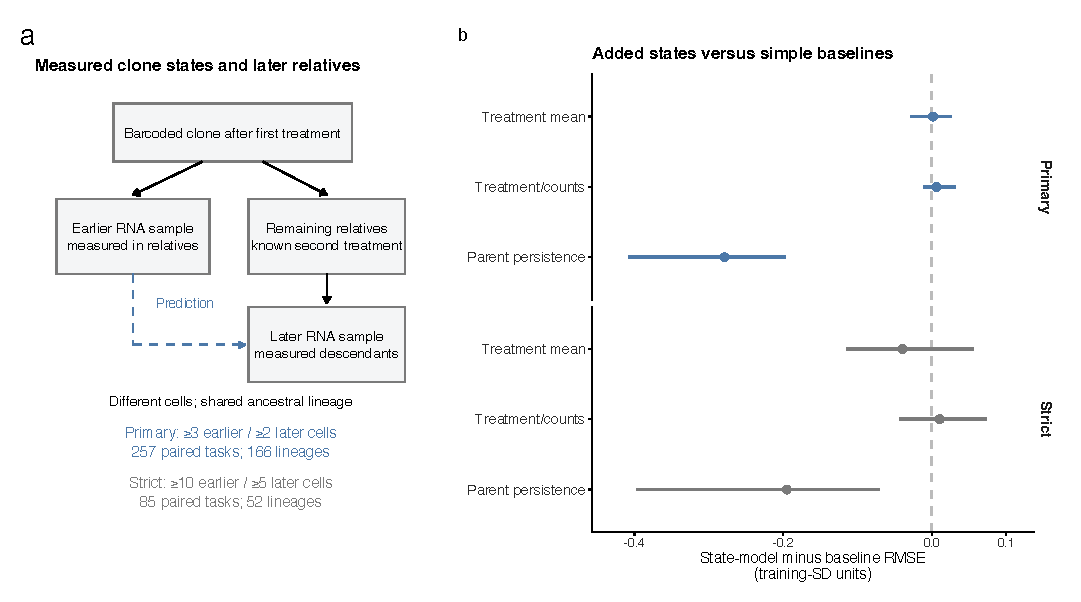
\includegraphics[width=\textwidth]{figure/SuppFig_independent_lineage.pdf}
\caption{\rev{\textbf{Earlier lineage state does not improve this conditional descendant-program prediction.} Measured parent and lineage-linked descendant profiles define the observation design.} \rev{Primary and strict support populations are shown separately.} \rev{State-minus-each-labelled-baseline RMSE intervals use 249 whole-lineage bootstrap draws, each repeating scaling, model fitting, penalty tuning and baseline selection.} \rev{Treatment/count ridge was the training-selected simple comparator in all five original folds in both support populations.} \rev{These intervals concern captured lineages within the source experiment and do not constitute independent culture replication.} \rev{Descendant cell support is a post-sampling covariate, precluding a pretreatment-policy interpretation.}}
\label{fig:supp-independent-lineage}
\end{figure}

\rev{Primary standardized joint RMSE was 0.96628 for treatment/count ridge and 0.97274 for state-augmented ridge.} \rev{The paired difference was 0.00646 ($95\%$ full-refitting lineage-bootstrap interval $[-0.01111,0.03258]$).} \rev{Strict-population errors were 0.99145 and 1.00206, with difference 0.01060 ($[-0.06219,0.07450]$).} \rev{Parent persistence alone was worse than the selected simple comparator.} \rev{No equivalence or absence of biological state dependence follows from these intervals.} 

\clearpage
\section*{\rev{Supplementary Note S12. Source-ordered response gradients and fixed-ranking utility}}

\rev{These retrospective checks extend Note S10 using previously examined RPE1 outcomes, with definitions and tests fixed before calculation.} \rev{They do not supply independent validation.} \rev{Unless specified otherwise, effects retain its ninety-member Hallmark score, 6,780-gene library and own-target numerator exclusion.} \rev{K562 and RPE1 are contexts from one Replogle study.}

\paragraph{\rev{Source-defined groups and the inferential family.}}
\rev{Genes were ordered by increasing signed K562 UPR effect, with exact ties broken by gene symbol.} \rev{Consecutive balanced groups contained 88, 88, 88, 87 and 87 genes; RPE1 effects did not determine their boundaries.} \rev{Outcomes were the RPE1 group means, medians and fractions above zero, the Q5--Q1 mean contrast, Kendall's $\tau_b$ between quintile and RPE1 effect, and the linear coefficient for integer quintile $1,\ldots,5$.} \rev{An increasing isotonic projection of the five observed means was descriptive and did not test monotonicity or determine candidate ranks.}

\rev{The three group tests and four priority-minus-unweighted-UPR Precision/NDCG comparisons formed one joint Holm family of seven (Table S8).} \rev{Two-sided tests used 10,000 gene-label permutations within the original source-expression-by-count strata, retaining the missing-expression stratum.} \rev{Statistics were centred on their permutation-null mean; this accommodates nonzero null contrasts induced by stratification.} \rev{Identical-list comparisons remained in the family.} \rev{The seven tests were also retained in the pooled 87-test BH sensitivity with the eighty curated-readout associations in Note S13.} \rev{Other ranking controls and sensitivities were descriptive.}

\rev{Two thousand whole-gene bootstrap draws used shared gene multiplicities across groups and methods.} \rev{Shared-GEM wild draws applied one Rademacher sign per technical GEM to centred, cell-count-weighted gene--GEM residuals.} \rev{Source groups and lists remained fixed; control references and standard deviations were conditioned upon.} \rev{Missing gene--GEM rows remained unobserved.} \rev{These units do not constitute independent cultures or quantify uncertainty in source selection.} \rev{Simultaneous $95\%$ max-$t$ intervals used the maximum standardized deviation across the four adjacent mean contrasts within each bootstrap draw.}

\subsection*{\rev{Supplementary Table S8. Source-defined quintiles and the joint seven-test family.}}

\begin{samepage}
\rev{\textbf{a, Observed RPE1 effects in the full 438-gene population.}}
\begin{center}
\begin{tabular}{lrlrr}
\toprule
\rev{Quintile} & \rev{Genes} & \rev{Mean effect ($95\%$ gene interval)} & \rev{Median} & \rev{Positive/total}\\
\midrule
\rev{Q1} & \rev{88} & \rev{$-0.4587\;[-0.5449,-0.3713]$} & \rev{$-0.3476$} & \rev{7/88}\\
\rev{Q2} & \rev{88} & \rev{$-0.1703\;[-0.2392,-0.1001]$} & \rev{$-0.0832$} & \rev{22/88}\\
\rev{Q3} & \rev{88} & \rev{$-0.0868\;[-0.1405,-0.0376]$} & \rev{$-0.0465$} & \rev{31/88}\\
\rev{Q4} & \rev{87} & \rev{$-0.0382\;[-0.0976,0.0235]$} & \rev{$-0.0272$} & \rev{38/87}\\
\rev{Q5} & \rev{87} & \rev{$-0.0679\;[-0.1602,0.0244]$} & \rev{$-0.0304$} & \rev{42/87}\\
\bottomrule
\end{tabular}
\end{center}
\end{samepage}

\medskip
\begin{samepage}
\rev{\textbf{b, Prespecified tests.}}
\begin{center}
\begin{tabular}{lrrlrr}
\toprule
\rev{Test} & \rev{Genes} & \rev{Estimate} & \rev{$95\%$ gene interval} & \rev{Raw $P$} & \rev{Holm $P$}\\
\midrule
\rev{Q5--Q1 mean} & \rev{438} & \rev{0.3908} & \rev{$[0.2661,0.5209]$} & \rev{0.000100} & \rev{0.000700}\\
\rev{Kendall $\tau_b$} & \rev{438} & \rev{0.2738} & \rev{$[0.2047,0.3436]$} & \rev{0.000100} & \rev{0.000700}\\
\rev{Ordinal slope} & \rev{438} & \rev{0.0915} & \rev{$[0.0639,0.1195]$} & \rev{0.000100} & \rev{0.000700}\\
\rev{$\Delta$Precision@10} & \rev{370} & \rev{0.0000} & \rev{$[0.0000,0.0000]$} & \rev{1.000000} & \rev{1.000000}\\
\rev{$\Delta$Precision@20} & \rev{370} & \rev{0.1500} & \rev{$[0.0000,0.3158]$} & \rev{0.046295} & \rev{0.138886}\\
\rev{$\Delta$NDCG@10} & \rev{370} & \rev{$-0.0690$} & \rev{$[-0.2517,0.0319]$} & \rev{0.032797} & \rev{0.131187}\\
\rev{$\Delta$NDCG@20} & \rev{370} & \rev{$-0.0423$} & \rev{$[-0.1927,0.0429]$} & \rev{0.160084} & \rev{0.320168}\\
\bottomrule
\end{tabular}
\end{center}
\end{samepage}

\rev{Response effects and the ordinal slope use control-standard-deviation units; ranking differences are agreement-weighted minus unweighted UPR on the same 370 genes.} \rev{Whole-gene intervals and stratified permutation tests use distinct conditional reference procedures.}

\rev{The overall gradient did not imply strictly increasing means.} \rev{Adjacent mean changes were 0.2884, 0.0834, 0.0487 and $-0.0297$, with simultaneous whole-gene intervals $[0.1490,0.4278]$, $[-0.0224,0.1893]$, $[-0.0523,0.1496]$ and $[-0.1702,0.1108]$.} \rev{All five means were nondecreasing in 22.25\% of gene draws, 0.40\% of shared-GEM wild draws and none of the 200 equal-100-cell draws.} \rev{These are resampling frequencies, not posterior probabilities or additional monotonicity tests.} \rev{Exact target-denominator correction retained Q5--Q1 of 0.3909; its equal-cell median was 0.3918, with central subsampling range $[0.3754,0.4080]$.} \rev{Fixed-primary-group projections into the 370- and 390-gene rosters gave Q5--Q1 contrasts of 0.3871 and 0.4160; separately defined within-cohort quintiles are reported with distinct labels.}

\paragraph{\rev{Fixed-list metrics and fair comparisons.}}
\rev{For an ordered source list $g_1,\ldots,g_K$, the fixed sign criterion and linear-gain metrics were
{}
{}
{\color{red}
\begin{align*}
\operatorname{Precision}@K&=\frac{1}{K}\sum_{j=1}^{K}\mathbf{1}\{d_{g_j}^{\mathrm{RPE1}}>0\},\\
r_g&=\max(d_g^{\mathrm{RPE1}},0),\qquad
\operatorname{DCG}@K=\sum_{j=1}^{K}\frac{r_{g_j}}{\log_2(j+1)},\\
\operatorname{NDCG}@K&=\frac{\operatorname{DCG}@K}{\operatorname{IDCG}@K}.
\end{align*}
}
}

\rev{Ideal gain is a same-cohort validation normalization, not a selection rule.} \rev{Zero remained fixed without validation-threshold optimization; positivity specifies direction rather than a minimum meaningful magnitude.} \rev{Rankings were source-fixed.} \rev{Method comparisons use 370 complete-comparator genes, with all-438 results separate.} \rev{Gene-bootstrap NDCG differences condition on observed ideal gain; technical-GEM draws recalculate effects, signs and ideal gain.}

\subsection*{\rev{Supplementary Table S9. Observed ranking metrics and definition sensitivity.}}

\begin{samepage}
\rev{\textbf{a, Fixed source rankings on the common 370-gene population.}}
\begin{center}
\begin{tabular}{lrrrr}
\toprule
\rev{Ranking/reference} & \rev{Precision@10} & \rev{Precision@20} & \rev{NDCG@10} & \rev{NDCG@20}\\
\midrule
\rev{UPR plus agreement} & \rev{0.90} & \rev{0.70} & \rev{0.3668} & \rev{0.3370}\\
\rev{Positive UPR effect} & \rev{0.90} & \rev{0.55} & \rev{0.4358} & \rev{0.3792}\\
\rev{Three-module magnitude} & \rev{0.00} & \rev{0.05} & \rev{0.0000} & \rev{0.0024}\\
\rev{Essentiality} & \rev{0.00} & \rev{0.00} & \rev{0.0000} & \rev{0.0000}\\
\rev{Control target expression} & \rev{0.20} & \rev{0.20} & \rev{0.0375} & \rev{0.0495}\\
\rev{Source cell count} & \rev{0.10} & \rev{0.20} & \rev{0.0019} & \rev{0.0095}\\
\rev{Annotation-derived significance} & \rev{0.20} & \rev{0.15} & \rev{0.1553} & \rev{0.1238}\\
\rev{Matched modules, median} & \rev{0.20} & \rev{0.30} & \rev{0.0424} & \rev{0.0548}\\
\rev{Uniform orderings, mean} & \rev{0.3052} & \rev{0.3054} & \rev{0.0590} & \rev{0.0728}\\
\bottomrule
\end{tabular}
\end{center}
\end{samepage}

\rev{Named-method entries are observed values for unchanged lists.} \rev{Reference entries summarize one hundred fixed expression/detection-matched modules or 10,000 uniform random orderings; they are not biological replicates.} \rev{Annotation-derived significance had a 217-way maximal-score tie, so its gene-symbol tie-broken Top $K$ is not a benchmark of the original authors' complete annotation method.} \rev{The full-panel positive prevalence was 140/438 (0.3196), compared with 113/370 (0.3054) in the common-comparator population.}

\medskip
\begin{samepage}
\rev{\textbf{b, Alternative-parent readouts and source-only priorities.}}
\begin{center}
\begin{tabular}{p{0.32\textwidth}rrrr}
\toprule
\rev{Readout} & \rev{\shortstack{Hallmark list\\Precision@20}} & \rev{\shortstack{Parent list\\Precision@20}} & \rev{\shortstack{Hallmark list\\gap}} & \rev{\shortstack{Parent list\\gap}}\\
\midrule
\rev{Reactome UPR, full} & \rev{0.70} & \rev{0.65} & \rev{0.3611} & \rev{0.3781}\\
\rev{Reactome UPR, disjoint} & \rev{0.60} & \rev{0.30} & \rev{0.1564} & \rev{$-0.0611$}\\
\rev{GO ER-UPR, full} & \rev{0.65} & \rev{0.45} & \rev{0.3777} & \rev{0.4213}\\
\rev{GO ER-UPR, disjoint} & \rev{0.65} & \rev{0.55} & \rev{0.1908} & \rev{0.2528}\\
\bottomrule
\end{tabular}
\end{center}
\end{samepage}

\rev{All entries in part b use exact target-count denominator exclusion and the common 370-gene population.} \rev{The Hallmark list uses the ninety-member Hallmark-defined source priority; the parent list uses the source priority for the corresponding alternative UPR definition.} \rev{Gaps are mean signed readout effects relative to each list's source-frozen matched background.} \rev{Disjoint memberships exclude the full approved-symbol Hallmark set.} \rev{These are descriptive sensitivity estimates; complete paired intervals and matching availability accompany Supplementary Data.}

\rev{The Hallmark-defined top-ten and top-twenty lists contained nine and fourteen positive RPE1 effects, compared with 28\% and 23\% in their frozen backgrounds.} \rev{Positive-fraction gaps were 0.62 and 0.47, with intact-matched-set intervals $[0.44,0.78]$ and $[0.29,0.64]$.} \rev{Agreement weighting did not demonstrate an advantage over the simple positive-UPR ranking after Holm correction (Table S8).} \rev{Identical top-ten membership gave identical Precision, whereas its different internal source order gave different NDCG.} \rev{Both UPR-directed rankings exceeded all one hundred original matched-module rankings on these Precision/NDCG endpoints; the agreement-weighted priority's finite-null upper-tail fraction was $1/101$.} \rev{Uniform-ordering reference means were also lower.} \rev{These are descriptive ranking calibrations for the specified RPE1 Hallmark readout, not tests of uniquely conserved pathway biology.}

\paragraph{\rev{Sequencing-depth diagnostic.}}
\rev{Across all 438 genes, one OLS model with an intercept related the ninety-member Hallmark RPE1 effect to per-target means of cell-level $\log(1+\mathrm{UMI})$ in K562 and RPE1; 2,000 shared whole-gene bootstrap draws refitted the model and recomputed fixed-list and matched-background weighted means.} \rev{K562/RPE1 standardized UMI differences were ($-0.152$, $0.138$) for the top ten and ($-0.096$, $-0.164$) for the top twenty, with adjusted residual matched gaps of 0.5780 ($95\%$ gene-bootstrap interval $[0.2131,0.8912]$) and 0.3474 ($[0.0725,0.5923]$) control standard deviations, respectively.} \rev{Because treated-cell UMI reflects measurement depth and biological RNA content, this conditional diagnostic does not establish causal benefit; source ranks, raw Precision/NDCG and the original test families were retained without additional tests.}

\rev{The strict 390-gene support rule retained eight of the original top ten and seventeen of the original top twenty.} \rev{Literal-list utility was therefore unestimable in that population: missing members were neither silently removed nor replaced.} \rev{The exact-denominator and equal-cell checks retained the original source ordering and lists.} \rev{Random-cell subsampling ranges quantify sensitivity to measured-cell support, rather than gene-sampling uncertainty.}

\paragraph{\rev{Alternative definitions and identifier coverage.}}
\rev{The four Reactome/GO full and Hallmark-disjoint definitions in Note S13 supplied additional source-only candidate sensitivities.} \rev{For each definition and normalization mode, priority remained $\max(d_g^{\mathrm{K562}},0)f_g$, where $f_g$ is the positive-contrast fraction among source GEMs containing at least five target cells.} \rev{Signed source effect and then gene symbol broke ties.} \rev{Alternative priorities, corresponding unweighted source-effect lists and source-only matches were frozen before reading the corresponding parent RPE1 effects; the Hallmark RPE1 outcomes had already been examined.} \rev{The Hallmark-defined lists and all original comparators were retained.}

\rev{Alternative definitions did not yield invariant priorities.} \rev{Exact-mode top-twenty overlap with the Hallmark list ranged from five to eleven genes in the full 438-gene population and five to twelve in the common 370-gene population.} \rev{Hallmark-list top-twenty matched gaps remained positive across all four parent readouts (Table S9b), but the Reactome-disjoint parent list gave $-0.0611$ with matched-set interval $[-0.2138,0.0849]$.} \rev{Neither agreement weighting nor the alternative-definition lists consistently improved on corresponding raw source effects.} \rev{Parent-specific random-module comparisons used fixed-library real and null readouts only; exact-normalization real results were not compared with those nulls.} \rev{For example, Hallmark-list Precision@20 of 0.65 on the GO-disjoint readout was ordinary relative to its matched parent-null rankings (upper-tail fraction 0.634).} \rev{All definitions, modes and negative or unavailable comparisons were retained without an additional formal testing family.}

\rev{A separate identifier-coverage sensitivity restored four unambiguously mapped original Hallmark members, giving ninety-four measured genes.} \rev{The source groups and lists defined by the ninety-member score were evaluated on that readout without deriving ninety-four-member rankings.} \rev{Exact-mode Precision@10/@20 remained 0.90/0.70; top-ten and top-twenty matched signed gaps were 0.5620 ($95\%$ matched-set interval $[0.2148,0.9504]$) and 0.3191 ($[0.0874,0.5680]$).} \rev{The unweighted ranking based on the ninety-member readout retained higher observed NDCG, and the upper-quintile mean downturn remained.} \rev{This sensitivity supplied no ninety-four-member null-specificity inference or additional formal $P$-value family; the ninety-member score remained the primary readout.}

\begin{figure}[H]
\centering
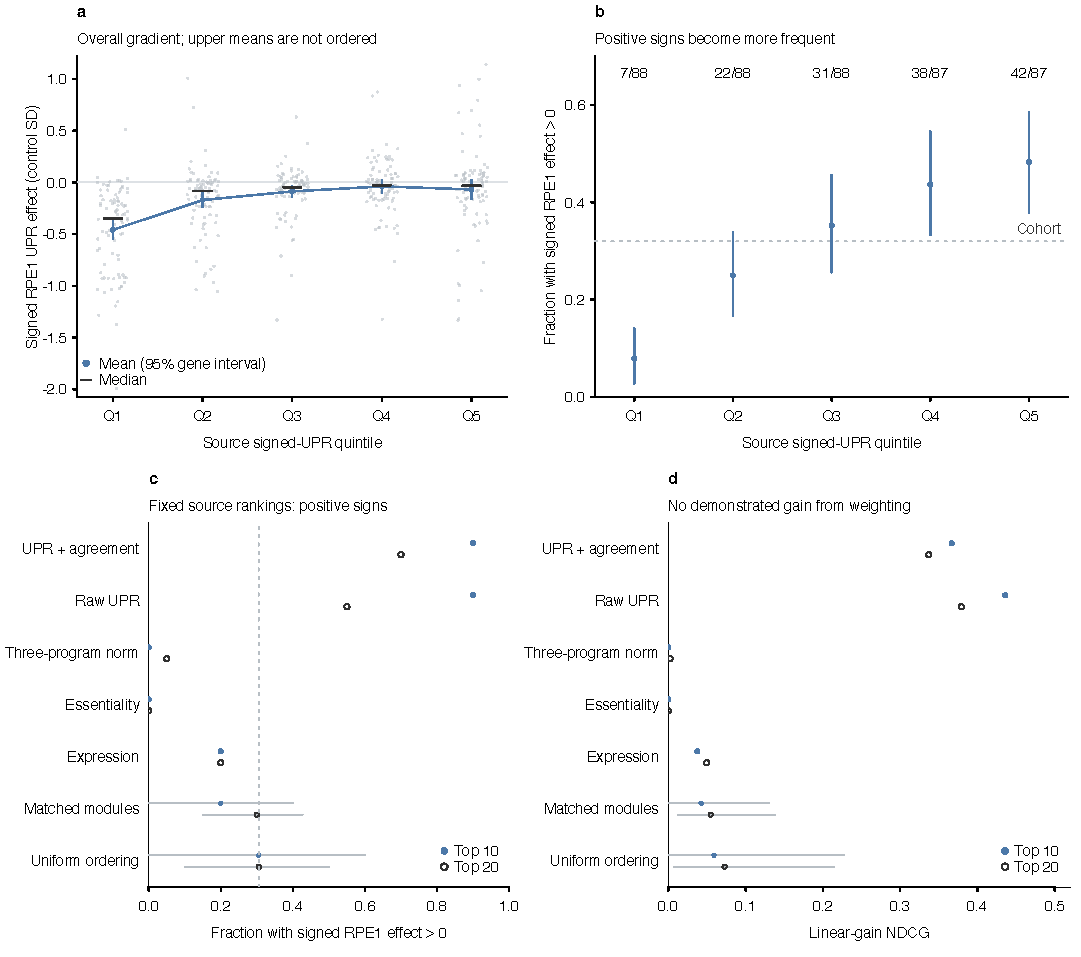
\includegraphics[width=\textwidth]{figure/Fig_UPR_quintiles_ranking_robustness.pdf}
\caption{\rev{\textbf{Source-UPR quintile gradients and fixed-ranking utility in previously evaluated RPE1 data.} \textbf{a}, The 438 metadata-eligible genes grouped by signed K562 UPR effect into fixed quintiles of 88, 88, 88, 87 and 87 genes.} \rev{Grey points denote genes; blue points and lines denote observed RPE1 means, bars are $95\%$ whole-gene bootstrap intervals, and black segments mark medians.} \rev{Means increase through Q4 and decrease in Q5; an overall trend does not establish strict monotonicity.} \rev{\textbf{b}, Fractions with signed RPE1 effect above zero and $95\%$ whole-gene intervals in the same population; labels give positive/total counts and the dotted line gives cohort prevalence.} \rev{\textbf{c,d}, Fixed top-ten (filled blue) and top-twenty (open black) source rankings on the common 370-gene comparator population.} \rev{Named-method points are observed Precision and linear-gain NDCG; paired gene/GEM intervals and Holm7 tests are given in Table S8 and Supplementary Data.} \rev{The dotted line in c denotes the 370-gene positive prevalence.} \rev{Bars on reference rows are central $95\%$ distributions across one hundred fixed expression/detection-matched modules or 10,000 uniform orderings, rather than biological confidence intervals.} \rev{Identical top-ten membership can give different NDCG because internal source order differs.} \rev{Precision uses the fixed sign threshold $d>0$; the validation-ideal ordering only normalizes NDCG.} \rev{RPE1 is another cellular context from the same study as K562.} \rev{These retrospective checks retain the original ranks and do not demonstrate a weighting advantage, functional activation or independent biological replication.}}
\label{fig:supp-upr-quintiles-ranking}
\end{figure}

\paragraph{\rev{Source data.}}
\rev{Complete numerical results and figure source data are listed in the collection's \nolinkurl{table_index.tsv}.} \rev{Code, execution records and computational draws accompany the separate reproducibility archive.}


\clearpage
\section*{\rev{Supplementary Note S13. Curated functional and alternative UPR readouts}}

\paragraph{\rev{Response ordering and functional specificity.}}

\rev{We tested whether the transported ordering identified a function-specific response using four GO processes and two alternative UPR definitions (Fig.~\ref{fig:upr-readout}).} \rev{Measured full readouts contained nine ER-folding, 67 ERAD, 34 ER-targeting and twenty ISR genes, with 69 Reactome-UPR and 41 GO-UPR genes.} \rev{In RPE1, folding, ERAD and ISR readouts retained positive correlations ($\rho=0.277$, 0.220 and 0.241; all BH $q<0.001$ across eighty tests), whereas the full ER-targeting result did not pass correction ($\rho=0.108$, $q=0.0585$).} \rev{Hallmark-disjoint folding, ERAD and ISR scores also retained positive RPE1 associations ($\rho=0.257$, 0.284 and 0.171; all $q<0.001$).} \rev{Direction agreement was modest: folding, ERAD and ISR concordance was 61.6\%, 55.3\% and 56.4\%, with chance-adjusted $\kappa=0.175$, 0.086 and 0.099.} \rev{Thus a positive rank correlation did not imply strongly preserved effect direction.}

\rev{An HGNC-resolved 94-member Hallmark readout retained the association ($\rho=0.392$; $95\%$ interval $[0.302,0.478]$), with unchanged top-ten/top-twenty sign precision; this was an identifier-coverage sensitivity rather than a new ranking.} \rev{Alternative curated definitions gave different results.} \rev{Full Reactome UPR correlated between K562 and RPE1 ($\rho=0.174$; $95\%$ interval $[0.070,0.274]$; $q=0.00104$), but its thirty-gene Hallmark-disjoint version did not ($\rho=-0.024$; $[-0.122,0.076]$; $q=0.760$).} \rev{GO-UPR retained correlations with its full and disjoint readouts ($\rho=0.185$ and 0.244; $q<0.001$).} \rev{Across the independent-study panels, Adamson supported several full functional and parent readouts, while unstimulated melanoma supported only full ERAD after the eighty-test correction.} \rev{No readout passed correction in the interferon-$\gamma$ panel.} \rev{Co-culture GO-UPR associations were positive, but these context patterns were not interpreted as a corrected immune-context interaction.} \rev{Full results, paired diagnostics and small-panel depth sensitivities are retained in Supplementary Note S13.}

\rev{The matched random-readout controls did not establish biological specificity in RPE1.} \rev{None of the eight prespecified readouts was exceptional relative to its one hundred size/expression/detection-matched random sets (upper-tail fractions 0.267--1.000).} \rev{Several associations persisted after count, depth or expression adjustment, but this did not distinguish them from shared transcriptional response variation.} \rev{The fixed Hallmark-derived top-twenty list nevertheless retained higher signed responses than its matched backgrounds under all four alternative parent readouts (descriptive gaps 0.156--0.378 control standard deviations).} \rev{This did not produce invariant candidate rankings: source top-twenty overlap with the original list ranged from five to eleven genes in the full 438-gene population, and alternative-definition priorities did not consistently outperform simple source effects or matched random-module rankings.} \rev{Selection utility was therefore specific to the RNA readout and metric, rather than evidence for a uniquely conserved UPR mechanism or a universal gene priority.}

\begin{figure}[H]
\centering
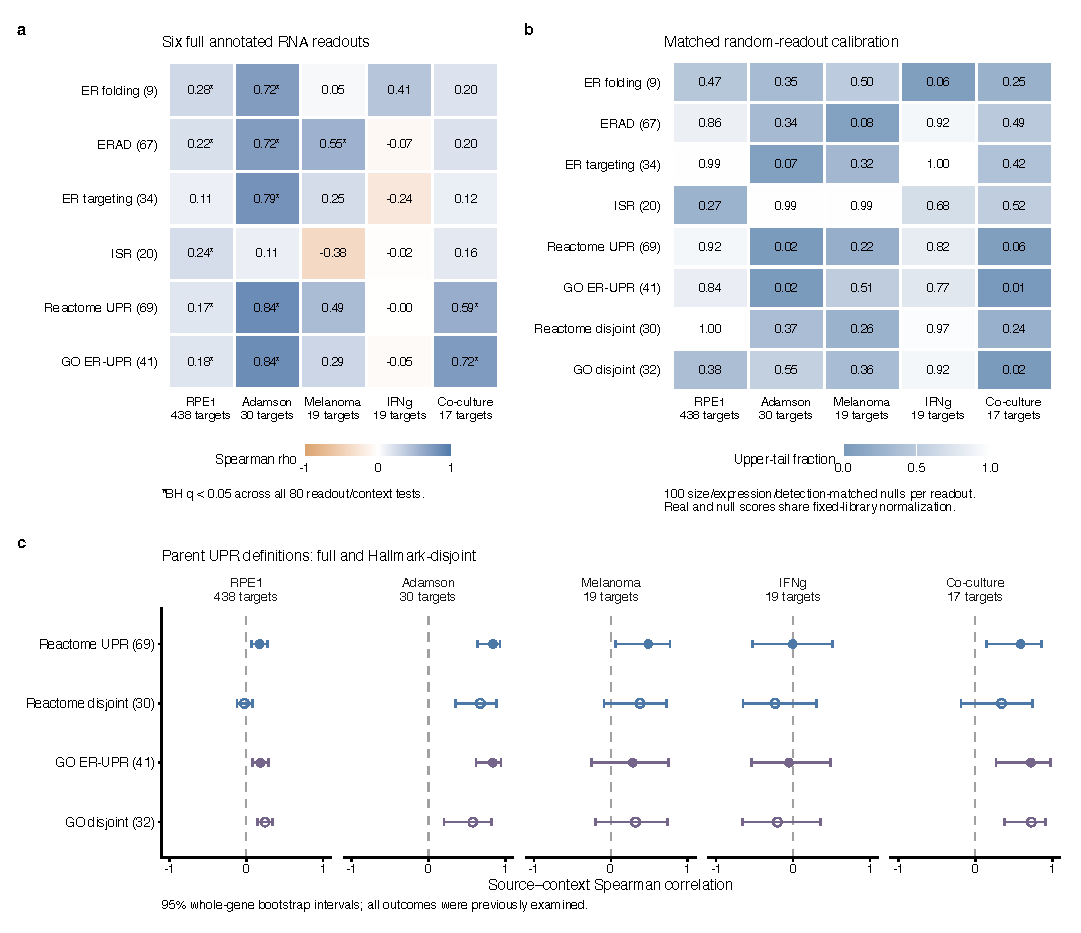
\includegraphics[width=\textwidth]{figure/Fig_UPR_readout_robustness.pdf}
\caption{\rev{\textbf{Curated readouts separate response ordering from biological specificity.} \textbf{a}, Source-to-context Spearman correlations for six full annotated RNA summaries; asterisks indicate BH $q<0.05$ across all sixteen full/disjoint/unique readouts in five contexts.} \rev{Numbers in parentheses denote measured readout genes.} \rev{\textbf{b}, Finite upper-tail fractions against one hundred size/expression/detection-matched random readouts per family; smaller values indicate more exceptional observed correlations.} \rev{These are descriptive calibration fractions, with real and null scores both using the fixed 6,780-gene denominator.} \rev{\textbf{c}, Full and canonical-Hallmark-disjoint Reactome/GO UPR correlations with 95\% whole-gene bootstrap intervals from 4,999 draws.} \rev{Panels a,c use exact target-count denominator and own-member numerator exclusion.} \rev{The target panels contain 438 RPE1, thirty Adamson, nineteen unstimulated/interferon-$\gamma$ melanoma and seventeen co-culture genes.} \rev{All outcomes had previously been examined; the prespecified definitions supply robustness analyses, not new independent validation or biochemical activity measurements.}}
\label{fig:upr-readout}
\end{figure}




\paragraph{\rev{Authoritative definitions and measurement coverage.}}
\rev{This analysis examined whether the Hallmark-associated ordering extended to annotated functional processes and alternative UPR definitions.} \rev{Memberships and statistical specifications were fixed before their corresponding response calculations.} \rev{The datasets and initial Hallmark results had already been examined, so these comparisons assess robustness within the existing studies.}

\rev{Four Gene Ontology (GO) processes represented ER protein folding, ER-associated degradation quality control, protein targeting to the ER and integrated stress response signaling.\cite{go2000,go2026}} \rev{Protein targeting to the ER comprised signal-directed co-translational and post-translational targeting/import, with general ER-to-Golgi vesicular transport outside its scope.} \rev{The ISR term included its PERK-, HRI-, GCN2- and PKR-related ontology descendants.} \rev{Alternative UPR definitions used Reactome R-HSA-381119.4 and GO:0030968.\cite{reactome2024}} \rev{These definitions describe different collections of annotated genes.}

\rev{GO annotations were retrieved from QuickGO using ontology release 2026-09-27 and annotation snapshot 2026-07-28 10:08.} \rev{Human UniProtKB protein-product annotations were propagated through \texttt{is\_a} and \texttt{part\_of}; \texttt{NOT} annotations and RNAcentral/ComplexPortal entries were excluded.} \rev{All remaining evidence classes, including electronic annotations, were retained.} \rev{Reactome database release 98 supplied recursively expanded pathway participants represented by UniProt \texttt{ReferenceGeneProduct} entities.} \rev{Gene products were resolved by unique HGNC UniProt identifiers, exact approved symbols and then unique previous/alias symbols.} \rev{The official HGNC complete-set file had HTTP last-modification date 2026-11-05 and was retrieved on 2026-11-06.} \rev{Its download metadata, raw contents and checksum are preserved; this is a dated snapshot rather than a numbered HGNC release.} \rev{Unresolved or ambiguous mappings remained explicit in the annotation tables.} \rev{Duplicate count features with the same assay symbol were summed before transformation, and no approved gene mapped to multiple columns within the fixed measurement universe.}

\rev{Each functional set was evaluated in full, after removing the complete approved-symbol Hallmark-UPR membership, and after removing members shared with any of the other three full functional sets.} \rev{Each alternative UPR parent was evaluated in full and after Hallmark removal. These operations preceded intersection with measured genes and produced sixteen fixed readouts (Supplementary Table S10).} \rev{Membership overlap makes these paired specifications dependent.} \rev{In particular, the measured ISR full and module-unique sets were identical, as were the measured ER-targeting Hallmark-disjoint and module-unique sets.} \rev{These repetitions do not provide additional biological replication.} \rev{Complete memberships, mapping decisions and overlap are supplied in \nolinkurl{authoritative_full_memberships.tsv}, \nolinkurl{GO_annotation_mapping.tsv} and \nolinkurl{hierarchy_and_overlap.tsv}.}

\subsection*{\rev{Supplementary Table S10. Curated and measured readout membership.}}

\begingroup
\small
\begin{center}
\begin{tabular}{p{0.25\textwidth}p{0.23\textwidth}rrrr}
\toprule
\rev{Readout} & \rev{Source identifier} & \rev{\shortstack[r]{Curated\\full}} & \rev{\shortstack[r]{Measured\\full}} & \rev{\shortstack[r]{Hallmark-\\disjoint}} & \rev{\shortstack[r]{Module-\\unique}}\\
\midrule
\rev{ER protein folding} & \rev{GO:0034975} & \rev{13} & \rev{9} & \rev{5} & \rev{4}\\
\rev{ERAD quality control} & \rev{GO:0036503} & \rev{96} & \rev{67} & \rev{59} & \rev{56}\\
\rev{ER targeting} & \rev{GO:0045047} & \rev{38} & \rev{34} & \rev{27} & \rev{27}\\
\rev{ISR signaling} & \rev{GO:0140467} & \rev{37} & \rev{20} & \rev{16} & \rev{20}\\
\rev{Reactome UPR} & \rev{R-HSA-381119.4} & \rev{92} & \rev{69} & \rev{30} & \rev{---}\\
\rev{GO ER-UPR} & \rev{GO:0030968} & \rev{64} & \rev{41} & \rev{32} & \rev{---}\\
\bottomrule
\end{tabular}
\end{center}
\endgroup

\rev{Curated counts denote mapped approved human genes before measurement restriction.} \rev{The other columns count measured genes after the specified membership operation.} \rev{Module uniqueness is defined only for the four functional sets.} \rev{No replacement genes were added after exclusions.}

\paragraph{\rev{Hallmark overlap and identifier coverage.}}
\rev{The original full Hallmark-UPR snapshot contained 113 genes.\cite{liberzon2015}} \rev{Approved-symbol mapping represented 94 of them in the assay universe.} \rev{This included four older assay symbols, H2AFX, IARS, TARS and TTC37, corresponding to H2AX, IARS1, TARS1 and SKIC3.} \rev{The primary ninety-member reference score retained its definition.} \rev{Full-membership exclusions and random-module sampling pools used the 94 mapped assay symbols.} \rev{The four added aliases were outside all sixteen curated readouts, so their inclusion in the exclusion dictionary did not change those real-readout memberships.} \rev{A separate identifier-coverage sensitivity evaluated the 94-member Hallmark readout, as described below.}

\paragraph{\rev{Count-level scores, control references and fixed panels.}}
\rev{All readouts retained the existing 6,780-gene normalization universe, although the metadata-only intersection of the four genetic studies contained 6,783 genes.} \rev{Let $x_{jc}$ be the raw count of measured gene $j$ in cell $c$, and let $U$ be the fixed universe.} \rev{For perturbation target $g$, the exact-normalization score for measured readout $A$ was
{}
{}
{\color{red}
\[
 L_c=\sum_{j\in U}x_{jc},\qquad
 L_c^{(-g)}=
 \begin{cases}
 L_c-x_{gc}, & g\in U,\\
 L_c, & g\notin U,
 \end{cases}
\]
}
}

\rev{{
{}
{\color{red}
\[
 s_{c,A}^{(-g)}=
 \frac{1}{|A\setminus\{g\}|}
 \sum_{j\in A\setminus\{g\}}
 \log\!\left(1+\frac{10^4x_{jc}}{L_c^{(-g)}}\right).
\]
}
}

\rev{Thus a target measurable only outside $U$ was not subtracted from that library.} \rev{Non-targeting controls were rescored separately for every target $g$, using the same numerator and denominator operations.} \rev{The resulting target-specific control distribution supplied its sample standard deviation and control means.} \rev{Each cell was scored only from measured members; absent features were not imputed as measured zeros.} \rev{Empty post-exclusion sets or nonpositive control standard deviations were unestimable.} \rev{Remaining-member counts were retained, with fewer than three members flagged as a few-transcript proxy.}}

\rev{In K562 and RPE1, each target's effect was the target-cell-count-weighted mean of treated-minus-control contrasts within matched GEMs, divided by the target-specific global control standard deviation.} \rev{All observed target GEMs contributed to that mean.} \rev{Adamson retained its global \texttt{63(mod)} non-targeting reference.} \rev{Its barcode capture-lane labels were retained as technical metadata and were not substituted for matched-GEM anchors.} \rev{Frangieh used pooled non-targeting cells within each condition.} \rev{The matched-reference choice was identical across real and random readouts.}

\rev{The external panels remained 438 RPE1 targets, thirty Adamson targets, nineteen Frangieh Control targets, nineteen interferon-$\gamma$ targets and seventeen co-culture targets.} \rev{K562 scoring retained the 467-gene union needed to supply these unchanged panels.} \rev{The count reconstruction included 98,052 K562 cells with 9,775 controls; 97,065 RPE1 cells with 11,485 controls; 27,599 Adamson cells with 6,284 controls; and 64,008 Frangieh cells with 57,605 controls.} \rev{The Frangieh count cache included the nineteen-target union; the condition-specific effect tables retained the fixed nineteen/nineteen/seventeen panels.} \rev{All 80 readout--comparison associations retained their designated target counts.}

\rev{Readout membership was also recorded separately as a perturbation-target annotation.} \rev{The RPE1 panel contained only one ER-folding, three ERAD, five ER-targeting and no ISR-annotated targets.} \rev{Adamson contained one, two, seven and one, respectively; the melanoma panels contained no targets in these four curated functional sets.} \rev{These small target strata were descriptive annotations, not replicated functional perturbation classes.}

\paragraph{\rev{Rank, direction and conditional association tests.}}
\rev{The sixteen readouts in five source--validation comparisons formed one eighty-test Spearman-correlation family.} \rev{Conditional 95\% intervals used 4,999 whole-gene bootstrap draws.} \rev{Two-sided Monte Carlo tests used 19,999 gene-label permutations, centered on the permutation mean and with the plus-one correction.} \rev{Permutation indices were shared across readouts when their panels agreed.} \rev{Benjamini--Hochberg correction covered all eighty hypotheses; raw $P$ values and four twenty-test subfamily identifiers were also retained.} \rev{Unavailable tests remained in the correction family with $P=1$, while their unestimable statistics remained missing.} \rev{The separate 87-test global sensitivity combined these eighty rank tests with the seven quintile/ranking comparisons described in Supplementary Note S12.}

\rev{Direction concordance was the fraction of nonzero pairs with matching effect signs.} \rev{Sign permutations preserved both source and validation sign marginals, rather than assuming a 50\% chance level.} \rev{Cohen's $\kappa$ and the Matthews correlation coefficient were reported with gene-bootstrap intervals.} \rev{A second summary was the mean source-sign-aligned validation shift,
{}
{}
{\color{red}
\[
 C_A=\frac{1}{n}\sum_g
 \operatorname{sign}\!\left(d_{g,A}^{\mathrm{K562}}\right)
 d_{g,A}^{\mathrm{validation}},
\]
}
}

\rev{where $d$ denotes the standardized gene effect.} \rev{Direction and $C_A$ tests formed one separate 160-test BH family.} \rev{The latter summarizes signed response consistency; it does not estimate calibrated cross-context effect amplitudes.} \rev{Zero effects and undefined agreement denominators were reported explicitly.}

\rev{Four separate rank-residual models assessed generic response covariates: source and validation log target-cell counts; source and validation non-targeting target-gene expression; source and validation three-short-module effect norms; and source and validation E2F effects.} \rev{The short-module and E2F effects were reconstructed with the same measurement universe and target corrections.} \rev{Control target expression used log1p CP10k with the fixed library.} \rev{Each model used complete cases and required at least three residual degrees of freedom.} \rev{Whole-gene bootstraps repeated residual fitting, and 19,999 Freedman--Lane permutations supplied conditional tests, with BH correction across all 320 readout--comparison--model combinations.} \rev{No model combined all covariates.} \rev{Expression-adjusted RPE1 comparisons retained 362 genes, distinct from the 370-gene comparator-matching population in Notes S10 and S12.} \rev{Complete-case counts and unavailable tests are supplied in \nolinkurl{all320_minimal_covariate_sensitivities.tsv}.}

\paragraph{\rev{Captured-RNA depth.}}
\rev{We averaged $\log(1+\mathrm{UMI})$ and, separately, $\log(1+L_c)$ for the frozen 6,780-gene count sum before target subtraction within each target's treated cells, then conditioned rank associations on the source and validation means for sixteen curated readouts and the fixed-library ninety-gene Hallmark reference across five panels (4,999 gene bootstraps, 19,999 Freedman--Lane permutations; joint BH170).} \rev{In RPE1, the Hallmark partial correlation was 0.347 ($95\%$ interval $[0.251,0.437]$) for recorded UMIs and 0.341 ($[0.247,0.431]$) for common-library counts (both $q=0.000236$), whereas Hallmark-disjoint Reactome remained uncertain ($-0.024$ [$-0.123,0.076$] and $-0.021$ [$-0.120,0.077$]; $q=0.812$ and 0.843).} \rev{Captured-RNA counts can reflect perturbation-induced RNA-content changes as well as technical support, so these conditional diagnostics differ from CP10k normalization and equal-cell resampling and neither isolate technical confounding nor rescue failed marginal or specificity tests.}
 \rev{The Hallmark reference retained its fixed-library outcome, whereas the sixteen curated readouts retained exact target-denominator correction; all fits used their complete designated target panels.} \rev{Full results are provided in \nolinkurl{sequencing_depth170_conditional_associations.tsv}.}

\rev{Paired specification and melanoma-context comparisons resampled complete target genes, carrying their matched responses together.} \rev{The three Frangieh conditions were not treated as independent studies.} \rev{A descriptive study-balanced $C_A$ summary first averaged the three melanoma conditions equally, then averaged that result, Adamson and RPE1 equally.} \rev{Its bootstrap retained gene-level context vectors and missingness; no missing outcome was replaced by zero.} \rev{This is not an independent-study common-effect meta-analysis.} \rev{Leave-one-target and leave-one-study-family summaries were retained as influence diagnostics.} \rev{The complete rank and direction families are supplied in \nolinkurl{primary80_rank_associations.tsv} and \nolinkurl{secondary160_direction_consistency.tsv}.}

\paragraph{\rev{Alternative UPR definitions and effect direction.}}
\rev{Full Reactome and GO UPR definitions had positive RPE1 associations, but their Hallmark-disjoint versions differed (Supplementary Table S11).} \rev{The Reactome disjoint estimate was $-0.024$ ($95\%$ interval $[-0.122,0.076]$; BH $q=0.760$), whereas the GO disjoint estimate was 0.244 ($[0.146,0.340]$; $q=0.000235$).} \rev{The full folding, ERAD and ISR RPE1 readouts also retained positive rank associations, with $\rho=0.277$, 0.220 and 0.241.} \rev{Their direction concordances were 61.6\%, 55.3\% and 56.4\%, with $\kappa=0.175$, 0.086 and 0.099.} \rev{Thus rank association did not ensure strong preservation of effect direction.} \rev{Only full ERAD passed BH80 in unstimulated melanoma, and no readout passed in the interferon-$\gamma$ panel.} \rev{The paired parent-UPR melanoma-context difference intervals all included zero; differences between marginal significance calls were not interpreted as an immune-context interaction.}

\subsection*{\rev{Supplementary Table S11. Full and Hallmark-disjoint parent-UPR associations.}}

\begingroup
\small
\begin{longtable}{p{0.22\textwidth}p{0.24\textwidth}p{0.34\textwidth}r}
\toprule
\rev{Validation panel} & \rev{Definition} & \rev{$\rho$ [95\% interval]} & \rev{BH80 $q$}\\
\midrule
\endhead
\rev{RPE1 (438)} & \rev{Reactome full} & \rev{$0.174\ [0.070,0.274]$} & \rev{0.00104}\\
\rev{} & \rev{Reactome disjoint} & \rev{$-0.024\ [-0.122,0.076]$} & \rev{0.760}\\
\rev{} & \rev{GO full} & \rev{$0.185\ [0.084,0.285]$} & \rev{0.000762}\\
\rev{} & \rev{GO disjoint} & \rev{$0.244\ [0.146,0.340]$} & \rev{0.000235}\\
\addlinespace
\rev{Adamson (30)} & \rev{Reactome full} & \rev{$0.838\ [0.638,0.929]$} & \rev{0.000235}\\
\rev{} & \rev{Reactome disjoint} & \rev{$0.673\ [0.346,0.882]$} & \rev{0.000600}\\
\rev{} & \rev{GO full} & \rev{$0.836\ [0.617,0.942]$} & \rev{0.000235}\\
\rev{} & \rev{GO disjoint} & \rev{$0.577\ [0.201,0.814]$} & \rev{0.00256}\\
\addlinespace
\rev{Melanoma Control (19)} & \rev{Reactome full} & \rev{$0.486\ [0.063,0.769]$} & \rev{0.0884}\\
\rev{} & \rev{Reactome disjoint} & \rev{$0.379\ [-0.089,0.723]$} & \rev{0.208}\\
\rev{} & \rev{GO full} & \rev{$0.286\ [-0.255,0.754]$} & \rev{0.405}\\
\rev{} & \rev{GO disjoint} & \rev{$0.321\ [-0.194,0.733]$} & \rev{0.333}\\
\addlinespace
\rev{Melanoma IFN-$\gamma$ (19)} & \rev{Reactome full} & \rev{$-0.004\ [-0.528,0.514]$} & \rev{0.989}\\
\rev{} & \rev{Reactome disjoint} & \rev{$-0.232\ [-0.650,0.302]$} & \rev{0.534}\\
\rev{} & \rev{GO full} & \rev{$-0.053\ [-0.537,0.488]$} & \rev{0.913}\\
\rev{} & \rev{GO disjoint} & \rev{$-0.204\ [-0.655,0.359]$} & \rev{0.589}\\
\addlinespace
\rev{Melanoma co-culture (17)} & \rev{Reactome full} & \rev{$0.591\ [0.146,0.861]$} & \rev{0.0323}\\
\rev{} & \rev{Reactome disjoint} & \rev{$0.341\ [-0.185,0.739]$} & \rev{0.333}\\
\rev{} & \rev{GO full} & \rev{$0.723\ [0.269,0.973]$} & \rev{0.00370}\\
\rev{} & \rev{GO disjoint} & \rev{$0.725\ [0.378,0.912]$} & \rev{0.00338}\\
\bottomrule
\end{longtable}
\endgroup

\rev{All estimates use exact target-count denominator and own-member numerator exclusion.} \rev{Intervals are conditional whole-gene-bootstrap percentiles and are not multiplicity-adjusted; $q$ values refer to the complete eighty-test family.} \rev{Parent full/disjoint variants are paired readouts on the same targets.}

\paragraph{\rev{Matched random readouts and technical support.}}
\rev{Eight readouts had one hundred matched random sets each: the four full functional sets, both full UPR parents and both Hallmark-disjoint UPR parents.} \rev{Random-set sizes equalled the measured real-readout sizes.} \rev{Each member was matched using five-by-five source-control expression/detection bins, excluding the tested readout and the full approved-symbol Hallmark membership.} \rev{Sampling was without replacement within a random set.} \rev{All 30,200 member draws matched exact bins; no bin expansion was needed.} \rev{The matching used the same 9,775 K562 non-targeting cells and no validation effects.}

\rev{Random-readout calibration used a separate fixed-library sensitivity.} \rev{Both real and random scores retained the same $L_c$, removed their own targeted member when applicable, and recomputed target-specific control moments.} \rev{These random sets do not calibrate the exact-denominator primary measurement.} \rev{Functional disjoint/unique variants without their own matched-size controls retained unresolved readout-specific calibration.} \rev{For observed statistic $T$, the finite upper-tail fraction was $(1+\#\{T_{\mathrm{null}}\geq T_{\mathrm{real}}\})/(1+N_{\mathrm{finite\ null}})$.} \rev{These fractions describe the available matched controls rather than a new permutation-test family.} \rev{RPE1 correlation fractions ranged from 0.267 to 1.000 across the eight calibrated readouts.} \rev{The complete distributions and finite counts are supplied in \nolinkurl{fixed_library_readout_specificity_calibration.tsv}.}

\rev{Technical-GEM sensitivity used 2,000 shared Rademacher draws, one weight per genuine GEM within each source/context block.} \rev{Gene-centered, observed-cell-weighted GEM residuals were perturbed with common weights across readouts; target-specific control standard deviations stayed fixed, and absent gene--GEM observations remained unobserved.} \rev{K562/RPE1 comparisons included genuine GEM variation in both contexts.} \rev{Adamson and Frangieh lacked corresponding genuine GEM metadata in this reconstruction, so their intervals varied source GEMs only and did not represent external technical uncertainty.}

\rev{Depth analyses sampled target cells without replacement in 200 draws, retaining the original target-specific control references and standard deviations.} \rev{The RPE1 analysis used one hundred target cells per gene in both contexts and retained all 438 genes for all sixteen readouts.} \rev{The smaller external panels used depths of thirty and fifteen.} \rev{At depth one hundred, the RPE1 folding correlation had median 0.259 and central 95\% subsampling range $[0.214,0.297]$.} \rev{Reactome-disjoint RPE1 ordering remained uncertain, with median $-0.0206$ and range $[-0.0726,0.0297]$; its shared-GEM percentile interval was $[-0.0784,0.0417]$.} \rev{The unstimulated-melanoma full-ERAD result was sampling sensitive: at thirty cells per target, median $\rho$ was 0.296 with range $[-0.175,0.597]$.} \rev{These ranges describe depth perturbation or conditional technical variation, not gene-sampling confidence intervals or independent culture replication.} \rev{Full results appear in \nolinkurl{equal_depth_signature_summaries.tsv} and \nolinkurl{shared_GEM_technical_signature_intervals.tsv}.}

\paragraph{\rev{Ninety-four-member identifier sensitivity and interpretation.}}
\rev{The identifier-coverage addendum fixed precisely the original ninety genes plus H2AFX, IARS, TARS and TTC37 before calculating their 94-member responses.} \rev{The four counts were recovered from the original matrices and aligned to the existing cells, library totals and target counts.} \rev{Both normalization modes used the same cohorts, control anchors and existing candidate lists; no 94-based ranking or new formal hypothesis family was introduced.} \rev{Primary inference continued to use the ninety-member readout.}

\rev{With exact target-count correction, the 94-member readout gave correlations 0.392 in RPE1 ($95\%$ interval $[0.302,0.478]$), 0.830 in Adamson, 0.616 in unstimulated melanoma, 0.053 under interferon-$\gamma$ and 0.475 in co-culture.} \rev{Paired 94-minus-90 gene-bootstrap intervals and direction diagnostics are retained in \nolinkurl{Hallmark94_identifier_sensitivity.tsv}.} \rev{Top-ten/top-twenty sign precision was unchanged.} \rev{Existing ninety-gene random modules were not relabeled as matched-size controls for the 94-member readout.}

\rev{These results delimit the biological interpretation.} \rev{Several annotated RNA readouts preserve some cross-context ordering, but agreement depends on definition, direction and the response background.} \rev{The failed Hallmark-disjoint Reactome measurement, nonexceptional RPE1 random-readout calibration and small-panel depth sensitivity limit support to definition-dependent RNA ordering.} \rev{Expression summaries do not measure folding capacity, ERAD flux, protein translocation, ISR kinase activation or functional benefit.} \rev{Conditional covariate associations and technical resampling refine the measured comparison; they do not supply a new independent experiment or replace a failed marginal endpoint.} \rev{Candidate projections under alternative definitions are reported in Supplementary Note S12.}



\clearpage
\section*{\rev{Supplementary Note S14. Frozen cross-study evaluation in HepG2}}

\paragraph{\rev{Independent measurement and analysis status.}}
\rev{The HepG2 CRISPRi experiment from GSE264667 was generated separately from the K562 discovery and RPE1 evaluation screens and reported by Nadig and colleagues.~\cite{nadig2025}} \rev{The studies share authors and perturbation technology; this is an unused cross-study experiment, not independent-laboratory replication.} \rev{Its expression outcomes had not entered the preceding model selection, UPR-axis selection, readout robustness or candidate rankings.} \rev{The evaluation specification was fixed before expression scoring, after accession-level metadata identified the experiment.} \rev{Jurkat was not read as a response-based fallback.} \rev{All original source effect values, ninety UPR members, candidate identities/order, simple comparators and one hundred source-matched random-module priorities were retained.}

\rev{The published matrix contained 145,473 cells and 9,624 measured features.} \rev{All ninety UPR members were measured, while 6,523 of the original 6,780 library genes were assayed.} \rev{The validation denominator was the count sum over those measured members; absent features were not imputed as zero and no readout member was replaced.} \rev{Duplicate assay symbols were summed before normalization.} \rev{This measurement difference prevents treating response amplitudes as an identically calibrated biological quantity across contexts.} \rev{The source priorities themselves were not recalculated.} \rev{The retained target/control roster contained 42,972 cells: 37,996 cells targeting the 438 frozen genes and 4,976 non-targeting cells.} \rev{Every technical GEM had controls, ranging from five to 123 cells; 56 GEM groups were represented.} \rev{Raw counts were checked for finite, nonnegative integer values and all retained common-library sums were positive.}

\rev{For every target, exact-count correction removed its raw counts from the assayed library when applicable and removed its own readout member.} \rev{Matched controls received identical numerator/denominator operations.} \rev{Treated-minus-matched-GEM control contrasts were weighted by target-cell counts and divided by the target-specific global control standard deviation.} \rev{A fixed-library measurement retained own-member exclusion as a separate sensitivity.} \rev{No validation response was used to refit source weights or define a new list.}

\paragraph{\rev{Support rules and multiplicity.}}
\rev{The primary threshold of thirty target cells and sixty non-targeting controls retained 417 genes.} \rev{Metadata alone showed seventeen GBF1 cells and twenty-four ALG14 cells.} \rev{Consequently, nine of ten and eighteen of twenty literal candidate identities met primary support, but neither complete list did.} \rev{The absent members were not replaced and partial-list metrics were not relabeled as Precision@10/@20.} \rev{Before expression outcomes were calculated, a metadata addendum specified one ten-cell sensitivity, retaining all 438 genes, alongside the original hundred-cell sensitivity with 106 genes.} \rev{These checks do not retrospectively change the primary threshold.}

\rev{The five primary hypotheses were source--validation signed rank association, two literal-list signed gaps against eligible nonselected genes and two weighted-minus-simple-UPR NDCG contrasts.} \rev{All five remained in Holm correction.} \rev{Unestimable effects remained missing; their $P=1$ entries are correction placeholders rather than completed null tests.} \rev{The rank test used 10,000 two-sided gene-label permutations with the plus-one correction.} \rev{Conditional 95\% whole-gene percentile intervals used 4,999 draws.} \rev{The primary association was $\rho=0.40258$, with interval $[0.31270,0.48888]$, raw $P=0.00009999$ and Holm $P=0.00049995$.} \rev{The remaining four primary statistics were unestimable.} \rev{These are all primary outcomes, not a selected positive subset.}

\paragraph{\rev{Additional metadata-only coverage search.}}
\rev{A subsequent search retained the original thirty-target-cell primary threshold, ninety-member RNA readout and frozen candidate identities.} \rev{No expression outcomes from the additional screens were evaluated.} \rev{Jurkat metadata from GSE264667 contained only eight GBF1 cells and measured 88 of the ninety readout members, excluding KDELR3 and VEGFA.} \rev{In the separate X-Atlas resource (dataset DOI: \nolinkurl{10.25452/figshare.plus.29190726}), guide-filtered HCT116 metadata contained 133 GBF1 and 229 ALG14 cells, but only 25 POLRMT and 27 RPL7 cells.} \rev{HEK293T metadata contained 103 GBF1 and 341 ALG14 cells, but only 29 RPS13 cells.} \rev{Guide-call counts are upper bounds on RNA-qualified support, not evidence of expression readout completeness.} \rev{GARS was matched to the guide-library symbol GARS1 (ENSG00000106105).} \rev{Neither X-Atlas context could support both complete frozen lists under the existing rule, even before RNA quality filtering.} \rev{Contexts were not pooled, candidates were not replaced, and no additional response comparison was performed.} \rev{These metadata findings leave the HepG2 low-support sensitivity and the unestimable primary complete-list endpoints unchanged.} \rev{All twenty candidate counts, metadata checksums and acquisition records accompany the reproducibility update.}

\subsection*{\rev{Supplementary Table S12. Response-ordering support and sensitivity.}}

\begin{center}
\begin{tabular}{lrrll}
\toprule
\rev{Normalization} & \rev{Minimum cells} & \rev{Genes} & \rev{$\rho$} & \rev{$95\%$ gene interval}\\
\midrule
\rev{Exact target exclusion} & \rev{30} & \rev{417} & \rev{0.403} & \rev{$[0.313,0.489]$}\\
\rev{Exact target exclusion} & \rev{10} & \rev{438} & \rev{0.424} & \rev{$[0.336,0.502]$}\\
\rev{Exact target exclusion} & \rev{100} & \rev{106} & \rev{0.449} & \rev{$[0.265,0.601]$}\\
\rev{Fixed library} & \rev{30} & \rev{417} & \rev{0.404} & \rev{$[0.314,0.486]$}\\
\rev{Fixed library} & \rev{10} & \rev{438} & \rev{0.425} & \rev{$[0.338,0.506]$}\\
\rev{Fixed library} & \rev{100} & \rev{106} & \rev{0.451} & \rev{$[0.273,0.598]$}\\
\bottomrule
\end{tabular}
\end{center}

\rev{Only the first row is the primary rank test.} \rev{Other rows are sensitivity estimates without a new formal testing family.} \rev{Direction concordance in the primary panel was 63.5\%; it does not establish a common biochemical mechanism or calibrated response magnitude.}

\paragraph{\rev{Frozen-list utility and comparator frames.}}
\rev{Precision counted effects strictly above zero.} \rev{Linear-gain NDCG used $\max(d,0)$ and $1/\log_2(r+1)$ discounts, with the validation-ideal gain calculated within the same comparison frame.} \rev{Primary literal-list membership came from the original 438-gene source roster.} \rev{The seven named comparator rankings used the same frozen 370-gene complete-source-covariate frame.} \rev{Missing validation support was reported, not filled with lower-ranked genes.} \rev{The ten-cell sensitivity retained all 370 genes and therefore permits direct observed-method comparisons.} \rev{Its weighted/simple NDCG@10 values were 0.57355/0.59369 and NDCG@20 values were 0.52513/0.56474.} \rev{Both methods had Precision@10/@20 of 0.80/0.75; the comparison-frame positive prevalence was 123/370.} \rev{Generic three-program magnitude gave Precision 0.10/0.15 and NDCG 0.04872/0.06463, while essentiality gave 0.10/0.05 and 0.03074/0.02462.} \rev{All remaining baselines are retained in the source tables.}

\rev{For the literal lists against all other genes in the 438-gene ten-cell frame, signed gaps were 0.51053 ($95\%$ gene interval $[0.28208,0.73351]$) and 0.34061 ($[0.19147,0.49283]$).} \rev{These are different reference populations from the complete-covariate comparator table, so their gaps and ideal gains are not silently interchanged.} \rev{Gene weights were shared across overlapping lists.} \rev{NDCG difference intervals conditioned on the observed ideal gain.} \rev{Raw conditional intervals are retained, together with intersections with the known metric parameter bounds; no interval was used to choose a method.} \rev{Neither the new data nor these descriptive comparisons supplied an observed advantage for agreement weighting over simple source effects.}

\rev{All one hundred expression/detection-matched source-module priorities predicted the same HepG2 UPR outcome; no missing module member was replaced by a newly selected response gene.} \rev{Under ten-cell support, every null list was estimable.} \rev{Both precision and NDCG for the UPR priorities exceeded all one hundred module-priority values, giving descriptive upper-tail fractions $1/101$.} \rev{Ten thousand uniform source orderings supplied an additional reference distribution.} \rev{These controls assess selection for the specified RNA readout, rather than proving that UPR is uniquely conserved.} \rev{The module memberships overlap and their one hundred outcomes are not independent biological replications.}

\paragraph{\rev{Conditional technical sensitivity.}}
\rev{Two thousand wild draws applied a shared Rademacher weight to each genuine GEM, perturbing gene-centred, target-cell-count-weighted GEM residuals while keeping absent gene--GEM observations absent.} \rev{Source effects, matched-control reference moments and control standard deviations were fixed.} \rev{The primary correlation's technical percentile range was $[0.331,0.406]$.} \rev{In the ten-cell sensitivity, top-ten/top-twenty signed-gap ranges were $[0.430,0.591]$ and $[0.290,0.393]$.} \rev{These ranges describe conditional technical perturbations; nonlinear rank attenuation makes them distinct from centred sampling confidence intervals.} \rev{They do not substitute for independent cultures or resolve the primary list-support shortfall.}

\subsection*{\rev{Supplementary Table S13. All frozen candidates and independent observed effects.}}

\begin{center}
\begin{tabular}{rlrrl}
\toprule
\rev{Source rank} & \rev{Gene} & \rev{HepG2 cells} & \rev{UPR effect} & \rev{Primary support}\\
\midrule
\rev{1} & \rev{POLRMT} & \rev{65} & \rev{0.314} & \rev{Yes}\\
\rev{2} & \rev{GBF1} & \rev{17} & \rev{0.628} & \rev{No}\\
\rev{3} & \rev{GMPPB} & \rev{36} & \rev{0.590} & \rev{Yes}\\
\rev{4} & \rev{RPS13} & \rev{148} & \rev{-0.074} & \rev{Yes}\\
\rev{5} & \rev{PNPT1} & \rev{47} & \rev{0.168} & \rev{Yes}\\
\rev{6} & \rev{UPF2} & \rev{37} & \rev{0.928} & \rev{Yes}\\
\rev{7} & \rev{SPCS3} & \rev{52} & \rev{0.667} & \rev{Yes}\\
\rev{8} & \rev{DNAJC19} & \rev{52} & \rev{-0.107} & \rev{Yes}\\
\rev{9} & \rev{MANF} & \rev{65} & \rev{0.154} & \rev{Yes}\\
\rev{10} & \rev{UFL1} & \rev{58} & \rev{0.670} & \rev{Yes}\\
\rev{11} & \rev{RBM10} & \rev{171} & \rev{-0.104} & \rev{Yes}\\
\rev{12} & \rev{ALG14} & \rev{24} & \rev{0.175} & \rev{No}\\
\rev{13} & \rev{RPL7} & \rev{122} & \rev{-0.414} & \rev{Yes}\\
\rev{14} & \rev{HSP90B1} & \rev{60} & \rev{0.077} & \rev{Yes}\\
\rev{15} & \rev{TIMM13} & \rev{70} & \rev{0.126} & \rev{Yes}\\
\rev{16} & \rev{NELFCD} & \rev{50} & \rev{0.311} & \rev{Yes}\\
\rev{17} & \rev{GARS} & \rev{79} & \rev{0.323} & \rev{Yes}\\
\rev{18} & \rev{SMARCB1} & \rev{81} & \rev{-0.097} & \rev{Yes}\\
\rev{19} & \rev{MFN2} & \rev{139} & \rev{0.021} & \rev{Yes}\\
\rev{20} & \rev{LETM1} & \rev{70} & \rev{0.044} & \rev{Yes}\\
\bottomrule
\end{tabular}
\end{center}

\rev{Effects use exact own-target numerator and denominator exclusion.} \rev{Seventeen GBF1 cells and twenty-four ALG14 cells remain visible; no replacement candidates were introduced.} \rev{Positive effects are transcriptional contrasts relative to matched controls, not functional intervention outcomes.}

\paragraph{\rev{Source data and interpretation.}}
\rev{The independent HepG2 Supplementary Data collection retains the frozen members/rankings, all support flags, all six association estimates, all five primary endpoints, every named/random comparator, raw and bounded interval records, technical sensitivities and exact figure data.} \rev{Complete commands, locks, download records, per-cell contrasts, numerical QA and computational draws accompany the separate reproducibility archive.} \rev{The supported extension is positive cross-study RNA-response ordering and secondary evidence for targeted selection.} \rev{Complete-list primary utility remains unevaluated under the original support criterion; a uniquely conserved UPR mechanism, an advantage from score complexity and functional benefit are not established.}

\begingroup
\color{black}
\colorlet{scolor}{black}
\hypersetup{citecolor=black,linkcolor=black,urlcolor=black}
\begin{thebibliography}{99}
\bibitem{replogle2022}
\rev{J.~M. Replogle, R.~A. Saunders, A.~N. Pogson, J.~A. Hussmann, A.~Lenail, A.~Guna, et~al., Mapping information-rich genotype--phenotype landscapes with genome-scale {Perturb-seq}, Cell 185 (2022) 2559--2575.e28.
\newblock \href {https://doi.org/10.1016/j.cell.2022.05.013} {\path{doi:10.1016/j.cell.2022.05.013}}.}

\bibitem{norman2019}
\rev{T.~M. Norman, M.~A. Horlbeck, J.~M. Replogle, A.~Y. Ge, A.~Xu, M.~Jost, et~al., Exploring genetic interaction manifolds constructed from rich single-cell phenotypes, Science 365 (2019) 786--793.
\newblock \href {https://doi.org/10.1126/science.aax4438} {\path{doi:10.1126/science.aax4438}}.}

\bibitem{mcfarland2020}
\rev{J.~M. McFarland, B.~R. Paolella, A.~Warren, K.~Geiger-Schuller, T.~Shibue, M.~Rothberg, et~al., Multiplexed single-cell transcriptional response profiling to define cancer vulnerabilities and therapeutic mechanism of action, Nature Communications 11 (2020) 4296.
\newblock \href {https://doi.org/10.1038/s41467-020-17440-w} {\path{doi:10.1038/s41467-020-17440-w}}.}

\bibitem{weinreb2020}
\rev{C.~Weinreb, A.~Rodriguez-Fraticelli, F.~D. Camargo, A.~M. Klein, Lineage tracing on transcriptional landscapes links state to fate during differentiation, Science 367 (2020) eaaw3381.
\newblock \href {https://doi.org/10.1126/science.aaw3381} {\path{doi:10.1126/science.aaw3381}}.}

\bibitem{yan2025}
\rev{R.~E. Yan, A.~Corman, L.~Katgara, X.~Wang, X.~Xue, Z.~Z. Gajic, et~al., Pooled {CRISPR} screens with joint single-nucleus chromatin accessibility and transcriptome profiling, Nature Biotechnology 43 (2025) 1628--1634.
\newblock \href {https://doi.org/10.1038/s41587-024-02475-x} {\path{doi:10.1038/s41587-024-02475-x}}.}

\bibitem{collectri2023}
\rev{S.~M{\"u}ller-Dott, E.~Tsirvouli, M.~Vazquez, R.~O. Ramirez~Flores, P.~Badia-I-Mompel, R.~Fallegger, et~al., Expanding the coverage of regulons from high-confidence prior knowledge for accurate estimation of transcription factor activities, Nucleic Acids Research 51 (2023) 10934--10949.
\newblock \href {https://doi.org/10.1093/nar/gkad841} {\path{doi:10.1093/nar/gkad841}}.}

\bibitem{scenic2017}
\rev{S.~Aibar, C.~Bravo Gonz{\'a}lez-Blas, T.~Moerman, V.~A. Huynh-Thu, H.~Imrichova, G.~Hulselmans, et~al., {SCENIC}: single-cell regulatory network inference and clustering, Nature Methods 14 (2017) 1083--1086.
\newblock \href {https://doi.org/10.1038/nmeth.4463} {\path{doi:10.1038/nmeth.4463}}.}

\bibitem{schubert2018}
\rev{M.~Schubert, B.~Klinger, M.~Kl{\"u}nemann, A.~Sieber, F.~Uhlitz, S.~Sauer, et~al., Perturbation-response genes reveal signaling footprints in cancer gene expression, Nature Communications 9 (2018) 20.
\newblock \href {https://doi.org/10.1038/s41467-017-02391-6} {\path{doi:10.1038/s41467-017-02391-6}}.}

\bibitem{liberzon2015}
\rev{A.~Liberzon, C.~Birger, H.~Thorvaldsd{\'o}ttir, M.~Ghandi, J.~P. Mesirov, P.~Tamayo, The molecular signatures database hallmark gene set collection, Cell Systems 1 (2015) 417--425.
\newblock \href {https://doi.org/10.1016/j.cels.2015.12.004} {\path{doi:10.1016/j.cels.2015.12.004}}.}

\bibitem{badia2022}
\rev{P.~Badia-I-Mompel, J.~V{\'e}lez~Santiago, J.~Braunger, C.~Geiss, D.~Dimitrov, S.~M{\"u}ller-Dott, et~al., {decoupleR}: ensemble of computational methods to infer biological activities from omics data, Bioinformatics Advances 2 (2022) vbac016.
\newblock \href {https://doi.org/10.1093/bioadv/vbac016} {\path{doi:10.1093/bioadv/vbac016}}.}

\bibitem{lopez2018scvi}
\rev{R.~Lopez, J.~Regier, M.~B. Cole, M.~I. Jordan, N.~Yosef, Deep generative modeling for single-cell transcriptomics, Nature Methods 15 (2018) 1053--1058.
\newblock \href {https://doi.org/10.1038/s41592-018-0229-2} {\path{doi:10.1038/s41592-018-0229-2}}.}

\bibitem{li2018overlap}
\rev{F.~Li, K.~L. Morgan, A.~M. Zaslavsky, Balancing Covariates via Propensity Score Weighting, Journal of the American Statistical Association 113 (2018) 390--400.
\newblock \href {https://doi.org/10.1080/01621459.2016.1260466} {\path{doi:10.1080/01621459.2016.1260466}}.}

\bibitem{gears2024}
\rev{Y.~Roohani, K.~Huang, J.~Leskovec, Predicting transcriptional outcomes of novel multigene perturbations with {GEARS}, Nature Biotechnology 42 (2024) 927--935.
\newblock \href {https://doi.org/10.1038/s41587-023-01905-6} {\path{doi:10.1038/s41587-023-01905-6}}.}

\bibitem{scgen2019}
\rev{M.~Lotfollahi, F.~A. Wolf, F.~J. Theis, {scGen} predicts single-cell perturbation responses, Nature Methods 16 (2019) 715--721.
\newblock \href {https://doi.org/10.1038/s41592-019-0494-8} {\path{doi:10.1038/s41592-019-0494-8}}.}

\bibitem{cpa2023}
\rev{M.~Lotfollahi, A.~Klimovskaia~Susmelj, C.~De~Donno, L.~Hetzel, Y.~Ji, I.~L. Ibarra, et~al., Predicting cellular responses to complex perturbations in high-throughput screens, Molecular Systems Biology 19 (2023) e11517.
\newblock \href {https://doi.org/10.15252/msb.202211517} {\path{doi:10.15252/msb.202211517}}.}

\bibitem{chemcpa2022}
\rev{L.~Hetzel, S.~B{\"o}hm, N.~Kilbertus, S.~G{\"u}nnemann, M.~Lotfollahi, F.~J. Theis, Predicting cellular responses to novel drug perturbations at a single-cell resolution, in: Advances in Neural Information Processing Systems, Vol.~35, 2022, pp. 26711--26722.}

\bibitem{txpert2026}
\rev{F.~Wenkel, W.~Tu, C.~Masschelein, H.~Shirzad, L.~Hodgson, I.~Bendidi, et~al., {TxPert}: using multiple knowledge graphs for prediction of transcriptomic perturbation effects, Nature Biotechnology (2026).
\newblock \href {https://doi.org/10.1038/s41587-026-03113-4} {\path{doi:10.1038/s41587-026-03113-4}}.}
\bibitem{go2000}
\rev{M.~Ashburner, C.~A.~Ball, J.~A.~Blake, D.~Botstein, H.~Butler, J.~M.~Cherry, et~al., Gene ontology: tool for the unification of biology, Nature Genetics 25 (2000) 25--29.
\newblock \href{https://doi.org/10.1038/75556}{\path{doi:10.1038/75556}}.}

\bibitem{go2026}
\rev{The Gene Ontology Consortium, The Gene Ontology knowledgebase in 2026, Nucleic Acids Research 54 (2026) D1779--D1792.
\newblock \href{https://doi.org/10.1093/nar/gkaf1292}{\path{doi:10.1093/nar/gkaf1292}}.}

\bibitem{reactome2024}
\rev{M.~Milacic, D.~Beavers, P.~Conley, C.~Gong, M.~Gillespie, J.~Griss, et~al., The Reactome Pathway Knowledgebase 2024, Nucleic Acids Research 52 (2024) D672--D678.
\newblock \href{https://doi.org/10.1093/nar/gkad1025}{\path{doi:10.1093/nar/gkad1025}}.}

\bibitem{nadig2025}
\rev{A.~Nadig, J.~M.~Replogle, A.~N.~Pogson, V.~Murthy, S.~A.~McCarroll, J.~S.~Weissman, et~al., Transcriptome-wide analysis of differential expression in perturbation atlases, Nature Genetics 57 (2025) 1228--1237.
\newblock \href{https://doi.org/10.1038/s41588-025-02169-3}{\path{doi:10.1038/s41588-025-02169-3}}.}

\end{thebibliography}
\endgroup

\end{document}
